% PedalScope Methods — the technical document. Generated fragments are
% \input from ../generated (the manifest's numbers, the parity run's
% numbers, the glossary); nothing numeric is typed here. Build:
% `make methods-docs`. Drift: CI regenerates ../generated and ../figures
% and fails on any diff. No third-party product is named in a finding, and
% nothing in this document says what a measurement sounds like.
\documentclass[11pt,a4paper]{article}
% Shared preamble for methods.tex (the technical document) and explained.tex
% (its lay companion). Engine: pdflatex (pinned in latexmkrc).
\usepackage[utf8]{inputenc}
\usepackage[T1]{fontenc}
% The kernel's own labels reach the generated fragments verbatim (a
% product recipe is "2f1−f2" with a true minus sign, a pitch is "C♯4"), so
% the characters the shipped vocabulary uses are declared once here for
% both documents rather than rewritten by a generator.
\DeclareUnicodeCharacter{2212}{\ensuremath{-}}
\DeclareUnicodeCharacter{266F}{\ensuremath{\sharp}}
\DeclareUnicodeCharacter{266D}{\ensuremath{\flat}}
\DeclareUnicodeCharacter{2026}{\dots}
\DeclareUnicodeCharacter{2248}{\ensuremath{\approx}}
\DeclareUnicodeCharacter{2264}{\ensuremath{\le}}
\DeclareUnicodeCharacter{2265}{\ensuremath{\ge}}
\DeclareUnicodeCharacter{00D7}{\ensuremath{\times}}
\DeclareUnicodeCharacter{03B4}{\ensuremath{\delta}}
\usepackage{lmodern}
\usepackage{amsmath,amssymb}
\usepackage{booktabs,longtable,array}
\usepackage{graphicx}
\usepackage[margin=24mm]{geometry}
\usepackage{xcolor}
\usepackage[numbers,sort&compress]{natbib}
% hyperref: every cross-reference, citation, glossary term, TOC entry and
% URL in the PDF is a clickable link; bookmarks mirror the sections.
\usepackage[colorlinks=true,linkcolor=blue!50!black,citecolor=blue!50!black,
  urlcolor=blue!50!black,linktoc=all,bookmarksnumbered=true,bookmarksopen=true,
  pdfusetitle,pdfpagemode=UseOutlines,breaklinks=true]{hyperref}
\hypersetup{pdfsubject={PedalScope measurement methods},pdfkeywords={swept sine, harmonic distortion, parity, reproducibility}}
% DOIs in the bibliography resolve as links (plainnat emits \doi{...}).
\providecommand{\doi}{}\renewcommand{\doi}[1]{\href{https://doi.org/#1}{doi:#1}}
\newcommand{\repo}{\url{https://github.com/PhaseDog/PedalScope}}
% The licence line both documents print in their front matter (ruled
% 2026-09-08): the holder as the app's About view states it, CC BY 4.0 for
% the document, MIT for the scripts, the mark excluded. One definition, two
% uses; the two URLs are hyperref links (the pdf job's census counts them).
\newcommand{\licenceline}{%
  \begin{center}\small
  \copyright{} 2026 Richard Hoge. This document is licensed under CC~BY~4.0
  (\url{https://creativecommons.org/licenses/by/4.0/}). The accompanying
  scripts are licensed under MIT
  (\url{https://opensource.org/license/mit}). PedalScope and its mark are
  not part of either grant.
  \end{center}}
\graphicspath{{../figures/}{../../UserGuide/assets/}}
\setlength{\parskip}{4pt plus 1pt}
\setlength{\parindent}{0pt}
% Terms: \term{key} prints the glossary name and links to the entry;
% \termas{key}{text} links custom text. Both are what the terms guard scans.
% GENERATED by gen_docs.py from terms.yaml — do not edit
\expandafter\newcommand\csname term@manifest\endcsname{methods manifest}
\expandafter\newcommand\csname term@parity\endcsname{parity test}
\expandafter\newcommand\csname term@sweep\endcsname{synchronized swept sine}
\expandafter\newcommand\csname term@rate-constant\endcsname{rate constant}
\expandafter\newcommand\csname term@synchronization\endcsname{synchronization condition}
\expandafter\newcommand\csname term@instantaneous-frequency\endcsname{instantaneous frequency}
\expandafter\newcommand\csname term@excited-band\endcsname{excited band}
\expandafter\newcommand\csname term@fundamental\endcsname{fundamental}
\expandafter\newcommand\csname term@harmonic-order\endcsname{harmonic order}
\expandafter\newcommand\csname term@clipping\endcsname{clipping}
\expandafter\newcommand\csname term@harmonic-response\endcsname{harmonic response}
\expandafter\newcommand\csname term@harmonic-pulse\endcsname{harmonic pulse}
\expandafter\newcommand\csname term@deconvolution\endcsname{deconvolution}
\expandafter\newcommand\csname term@inverse-filter\endcsname{inverse filter}
\expandafter\newcommand\csname term@impulse-response\endcsname{impulse response}
\expandafter\newcommand\csname term@extraction-window\endcsname{extraction window}
\expandafter\newcommand\csname term@input-normalized\endcsname{input-normalized}
\expandafter\newcommand\csname term@validity-bound\endcsname{validity bound}
\expandafter\newcommand\csname term@alias-image\endcsname{alias image}
\expandafter\newcommand\csname term@thd\endcsname{total harmonic distortion}
\expandafter\newcommand\csname term@floor\endcsname{measurement floor}
\expandafter\newcommand\csname term@fundamental-presence\endcsname{fundamental presence}
\expandafter\newcommand\csname term@shaping\endcsname{harmonic shaping}
\expandafter\newcommand\csname term@coherence\endcsname{coherence}
\expandafter\newcommand\csname term@scatter\endcsname{read scatter}
\expandafter\newcommand\csname term@averaging\endcsname{sweep averaging}
\expandafter\newcommand\csname term@derotation\endcsname{derotation}
\expandafter\newcommand\csname term@tanh\endcsname{tanh}
\expandafter\newcommand\csname term@phantom\endcsname{phantom capture}
\expandafter\newcommand\csname term@decibel\endcsname{decibel}
\expandafter\newcommand\csname term@dbfs\endcsname{dBFS}
\expandafter\newcommand\csname term@dbc\endcsname{dBc}
\expandafter\newcommand\csname term@transfer-curve\endcsname{transfer curve}
\expandafter\newcommand\csname term@averaged-cycle\endcsname{averaged cycle}
\expandafter\newcommand\csname term@static-curve\endcsname{static curve}
\expandafter\newcommand\csname term@box-normalization\endcsname{box normalization}
\expandafter\newcommand\csname term@lobe-area\endcsname{unsigned lobe area}
\expandafter\newcommand\csname term@fundamental-ellipse\endcsname{fundamental ellipse}
\expandafter\newcommand\csname term@nonlinear-loop-area\endcsname{nonlinear loop area}
\expandafter\newcommand\csname term@phase-removal\endcsname{phase removal}
\expandafter\newcommand\csname term@frame-fit\endcsname{frame fit}
\expandafter\newcommand\csname term@lattice\endcsname{memoryless lattice}
\expandafter\newcommand\csname term@pairing-residual\endcsname{pairing residual}
\expandafter\newcommand\csname term@polarity\endcsname{polarity}
\expandafter\newcommand\csname term@orientation\endcsname{orientation resolution}
\expandafter\newcommand\csname term@coupling-capacitor\endcsname{coupling capacitor}
\expandafter\newcommand\csname term@alignment-error\endcsname{residual alignment error}
\expandafter\newcommand\csname term@memory-verdict\endcsname{memory verdict}
\expandafter\newcommand\csname term@two-tone\endcsname{two-tone measurement}
\expandafter\newcommand\csname term@intermodulation-product\endcsname{intermodulation product}
\expandafter\newcommand\csname term@product-order\endcsname{product order}
\expandafter\newcommand\csname term@analysis-lattice\endcsname{analysis lattice}
\expandafter\newcommand\csname term@reduced-ratio\endcsname{reduced tone ratio}
\expandafter\newcommand\csname term@lattice-spacing\endcsname{lattice spacing}
\expandafter\newcommand\csname term@lattice-snap\endcsname{lattice snap}
\expandafter\newcommand\csname term@coherent-sampling\endcsname{coherent sampling}
\expandafter\newcommand\csname term@analysis-window\endcsname{analysis window}
\expandafter\newcommand\csname term@local-floor\endcsname{local floor}
\expandafter\newcommand\csname term@capture-floor\endcsname{capture floor}
\expandafter\newcommand\csname term@gate\endcsname{presence gate}
\expandafter\newcommand\csname term@product-reading\endcsname{product reading}
\expandafter\newcommand\csname term@coherence-check\endcsname{coherence check}
\expandafter\newcommand\csname term@coherence-detector\endcsname{coherence detector}
\expandafter\newcommand\csname term@pair-statistic\endcsname{sideband pair statistic}
\expandafter\newcommand\csname term@harmonic-role\endcsname{harmonic role}
\expandafter\newcommand\csname term@just-ratio\endcsname{just ratio}
\expandafter\newcommand\csname term@gain-map\endcsname{gain map}
\expandafter\newcommand\csname term@drive-level\endcsname{drive level}
\expandafter\newcommand\csname term@level-lattice\endcsname{level lattice}
\expandafter\newcommand\csname term@drive-window\endcsname{drive window}
\expandafter\newcommand\csname term@map-cell\endcsname{cell}
\expandafter\newcommand\csname term@export-grid\endcsname{export grid}
\expandafter\newcommand\csname term@truncated-column\endcsname{truncated column}
\expandafter\newcommand\csname term@edge-mask\endcsname{edge mask}
\expandafter\newcommand\csname term@delivered-fundamental\endcsname{delivered fundamental}
\expandafter\newcommand\csname term@floor-stamp\endcsname{calibration stamp}
\expandafter\newcommand\csname term@median-read\endcsname{median read}
\expandafter\newcommand\csname term@drive-term\endcsname{drive term}
\expandafter\newcommand\csname term@operative-floor\endcsname{operative floor}
\expandafter\newcommand\csname term@analyzer-residue\endcsname{analyzer residue}
\expandafter\newcommand\csname term@composed-margin\endcsname{composed margin}
\expandafter\newcommand\csname term@corroborated-peak\endcsname{corroborated peak}
\expandafter\newcommand\csname term@peak-tile\endcsname{peak tile}
\expandafter\newcommand\csname term@cleanup-reading\endcsname{cleanup reading}
\expandafter\newcommand\csname term@audition-model\endcsname{audition model}
\expandafter\newcommand\csname term@leakage-map\endcsname{leakage map}
\expandafter\newcommand\csname term@compression-curve\endcsname{compression curve}
\expandafter\newcommand\csname term@probe-grid\endcsname{probe grid}
\expandafter\newcommand\csname term@fine-window\endcsname{fine window}
\expandafter\newcommand\csname term@stepped-tone\endcsname{stepped tone}
\expandafter\newcommand\csname term@settle-window\endcsname{settle region and measurement window}
\expandafter\newcommand\csname term@cycle-snap\endcsname{cycle snap}
\expandafter\newcommand\csname term@one-bin-estimator\endcsname{one-bin estimator}
\expandafter\newcommand\csname term@noise-stamp\endcsname{noise stamp}
\expandafter\newcommand\csname term@noise-gate\endcsname{per-step noise gate}
\expandafter\newcommand\csname term@incremental-slope\endcsname{incremental slope}
\expandafter\newcommand\csname term@hinge-fit\endcsname{hinge fit}
\expandafter\newcommand\csname term@knee\endcsname{knee}
\expandafter\newcommand\csname term@bound-zone\endcsname{floor-bound zone}
\expandafter\newcommand\csname term@resolution-band\endcsname{resolution band}
\expandafter\newcommand\csname term@unity-guard\endcsname{unity guard}
\expandafter\newcommand\csname term@noise-bound\endcsname{noise bound}
\expandafter\newcommand\csname term@floor-class\endcsname{floor class}
\expandafter\newcommand\csname term@floor-runs\endcsname{floor runs}
\expandafter\newcommand\csname term@null-run-reference\endcsname{null-run reference}
\expandafter\newcommand\csname term@floor-source\endcsname{floor source}
\expandafter\newcommand\csname term@summed-presence\endcsname{summed presence reading}

% The machine floor (ruled 2026-09-22, py/machine_floor.py): a measured
% deviation under \machineFloor{} is printed as the bound "≤ floor", and
% the sentence each parity section states once is defined here, once.
% GENERATED by gen_docs.py from machine_floor.py — do not edit
\newcommand{\machineFloor}{1e-10}
\newcommand{\machineFloorWords}{a ten-billionth}
\newcommand{\sidecarFigures}{12}

\newcommand{\machineFloorNote}{A measured figure under \machineFloor{} is
printed as the bound $\le$\,\machineFloor: below it the digits are the
machine's last-bit arithmetic rather than the method's, and two machines
running the same code do not share them. A stated tolerance keeps its
digits.}
\newcommand{\term}[1]{\hyperlink{term:#1}{\csname term@#1\endcsname}}
\newcommand{\termas}[2]{\hyperlink{term:#1}{#2}}
\newcommand{\code}[1]{\texttt{#1}}
\newcommand{\dB}{\ensuremath{\,\mathrm{dB}}}

\title{PedalScope Methods\\\large Technical reference: how each measurement is made, and how to check it}
\author{PedalScope}
\date{}

\begin{document}
\maketitle

\begin{abstract}
This document states, for each measurement PedalScope makes, exactly what
the shipping code computes: the stimulus, the analysis pipeline step by step
with its equations, every parameter that determines the result, and the
limits of what the result can claim. Every number in it is generated from a
machine-readable \term{manifest} emitted by the shipped code (the source is
open: \repo), every method is
reimplemented independently in Python from that manifest and the published
definition, and a continuous-integration \term{parity} test holds the two
implementations to each other and to analytic ground truth. A method change
in the app that the Python does not follow is a failing build, not a stale
page.
\end{abstract}
\licenceline

\tableofcontents
\clearpage

\section{How to read this document, and how to trust it}

\subsection{The pipeline behind the pages}
\begin{enumerate}
  \item \textbf{The manifest.} \code{analysisdump manifest} (a package tool
  built on the app's own measurement kernel) emits
  \code{Docs/Methods/generated/manifest.json}: one object per measurement, every
  parameter obtained by calling the shipped function that owns it, never by
  transcription. Where a parameter is a function rather than a number --- a
  window shape, a gate --- the manifest records its name, its defining
  constants and a one-line rule.
  \item \textbf{The reimplementation.} \code{Docs/Methods/py/harmonic\_distortion.py}
  is the method written again, from the manifest and the published
  definition~\citep{farina2000,novak2015}, not from the Swift; each further
  chapter has its own (\code{transfer\_curve.py} for the Transfer Curve,
  \code{gain\_map.py} for the Gain Map, which imports the first,
  \code{compression\_curve.py} for Compression, which imports the first's devices
  and noise and the transfer module's filters, and \code{chord\_imd.py}
  for Chord IMD).
  It produces the same table the shipped tool produces.
  \item \textbf{The parity test.} \code{test\_parity\_hd.py} (and, per
  chapter, its sibling) runs the shipped code and the Python on identical
  synthetic devices and asserts, at every valid point, that they agree to
  a stated tolerance and that both agree with analytic truth to a stated
  tolerance. Tolerances were set from measured distributions and are quoted
  in \S\ref{sec:hd-example}, \S\ref{sec:transfer-example},
  \S\ref{sec:compression-example}, \S\ref{sec:journey-example} and
  \S\ref{sec:imd-example}.
  \item \textbf{The figures} are generated by the Python, seeded and
  byte-stable; the UI captures are rendered headlessly from the app's own
  chart views by the user-guide pipeline.
  \item \textbf{The drift check.} CI regenerates the manifest, the fragments
  and the figures and fails on any difference from the committed copies, so
  what this document states is what the build computed.
\end{enumerate}

\subsection{What this document does not do}
It does not describe what any measurement sounds like. A measured difference
is a measured difference; whether it can be heard is a question the
instrument does not answer, and no sentence here claims otherwise. It names
no third-party product in a finding.

\section{Notation and conventions}
\label{sec:notation}

\begin{longtable}{@{}lp{0.72\linewidth}@{}}
\toprule Symbol & Meaning \\ \midrule \endhead
$f_s$ & the sample rate, Hz \\
$f_1, f_2$ & the sweep's start and end frequencies, Hz \\
$L$ & the sweep's \term{rate-constant}, s: $f(t) = f_1 e^{t/L}$ \\
$T$ & the sweep's actual duration, $T = L\ln(f_2/f_1)$ \\
$A$ & the sweep amplitude, linear, $1 = $ digital full scale \\
$\varphi(t)$ & the sweep's instantaneous phase, rad \\
$f(t)$ & the sweep's \term{instantaneous-frequency}, Hz \\
$k$ & a \term{harmonic-order}; $k = 1$ is the fundamental \\
$K$ & the highest order extracted \\
$f_0$ & a \term{fundamental} frequency, Hz --- the excitation whose $k$-th harmonic is read \\
$H_k(f)$ & the \term{harmonic-response} of order $k$ on the output-frequency axis (\S\ref{sec:hd-reading}) \\
$\Delta t_k$ & the time advance of order $k$'s \term{harmonic-pulse}: $L\ln k$ \\
$N$ & the deconvolution DFT length; $M$ the per-order response DFT length \\
$T_k$ & the \term{extraction-window} duration for order $k$ \\
$h[n]$ & the deconvolved \term{impulse-response}, circular over $N$ samples \\
dB re input & $20\log_{10}|H_k|$ --- \term{input-normalized}: a unit-gain linear device reads $H_1 = 1$, i.e.\ $0\dB$ \\
\term{dbfs} & dB relative to digital full scale \\
\term{dbc} & dB relative to a carrier (here, the louder played tone or the fundamental) \\
\bottomrule
\end{longtable}

Angles are radians. Logarithms are natural unless written $\log_{10}$.
Time-domain indices are integers $n = 0 \ldots N-1$; ``circular'' means
modulo the buffer length. A raised cosine is $\tfrac12(1 - \cos\theta)$
rising or $\tfrac12(1 + \cos\theta)$ falling.

\section{Harmonic Distortion}
\label{sec:hd}

\subsection{Purpose, and what the measurement cannot tell you}
Harmonic Distortion characterises how a device converts a single input
frequency into output at integer multiples of it: for every fundamental
$f_0$ in the swept band and every order $k \le K$, the amplitude the device
emits at $k f_0$, normalized by the input amplitude. One \term{sweep}
captures the whole band at one drive level; the result is $K$ frequency
responses $H_1(f) \ldots H_K(f)$ and the derived \term{thd} curve.

What it cannot tell you, stated once: (a) anything about behaviour at other
drive levels --- one sweep is one operating point; the Gain Map and
Compression measurements own the level axis; (b) anything about intermodulation
between two simultaneous notes --- Chord IMD owns that; (c) whether a read
in an order is content the circuit shaped or noise that landed in that
order's analysis window --- the \term{shaping} predicate reads that
separately (\S\ref{sec:hd-shaping}); (d) anything below the rig's own
\term{floor} (\S\ref{sec:hd-floor}); and (e) anything about what the
distortion sounds like.

\subsection{The stimulus}
\label{sec:hd-stimulus}
The stimulus is a synchronized exponential sine sweep~\citep{novak2015,
novak2010}:
\begin{equation}
  x[n] = A\,\sin\varphi(t_n),\qquad
  \varphi(t) = 2\pi f_1 L\left(e^{t/L} - 1\right),\qquad
  t_n = n/f_s,\; n = 0 \ldots \lfloor T f_s + \tfrac12\rfloor - 1 .
  \label{eq:sweep}
\end{equation}
Its instantaneous frequency is $f(t) = f_1 e^{t/L}$, so the sweep reaches
$f_2$ at $T = L\ln(f_2/f_1)$. The rate constant is not free: the
\term{synchronization} requires $f_1 L$ to be an integer, so for a
requested duration $\hat T$
\begin{equation}
  L = \frac{\max\!\big(1,\ \mathrm{round}(f_1 \hat T / \ln(f_2/f_1))\big)}{f_1},
  \label{eq:sync}
\end{equation}
which is what makes the $k$-th harmonic generated by a memoryless
nonlinearity an exact time-advanced copy of the sweep, advanced by
\begin{equation}
  \Delta t_k = L \ln k ,
  \label{eq:delay}
\end{equation}
and therefore separable in the deconvolved response with meaningful phase.
The first $\lfloor t_{\mathrm{in}} f_s \rfloor$ samples are scaled by a
rising raised cosine and the last $\lfloor t_{\mathrm{out}} f_s \rfloor$ by a
falling one. The fades bound the \term{excited-band}: below $f(t_{\mathrm{in}})$
and above $f(T - t_{\mathrm{out}})$ the device was driven under a ramp, and
reads there are properties of the measurement, not the device.

\begin{figure}[htbp]
  \centering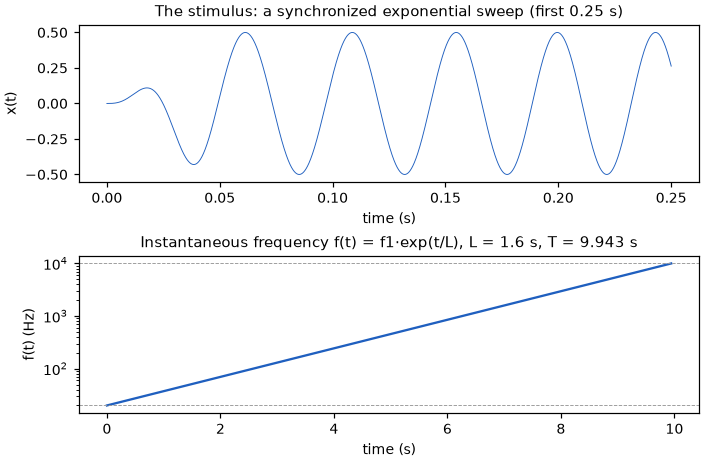
\includegraphics[width=0.9\linewidth]{hd-sweep.png}
  \caption{The stimulus, from the reimplementation: the waveform's first
  quarter second and the instantaneous frequency over the full sweep.}
\end{figure}

\subsection{The pipeline}
\label{sec:hd-pipeline}
Given the captured response $y[n]$, time-aligned with the sweep's start (the
app measures and removes the loop latency per capture before analysis; the
oracle runs at zero latency):

\begin{enumerate}
\item \textbf{\term{deconvolution} with the analytic inverse.} Zero-pad $y$
to $N$, the smallest power of two not less than the capture length plus
$\lfloor 0.1 f_s\rfloor$, and take its DFT $Y[m]$. The \term{inverse-filter}
is the stationary-phase closed form~\citep{novak2015}
\begin{equation}
  \tilde X^{-1}(f) = 2\sqrt{f/L}\;\exp\!\Big(j\big(\tfrac{\pi}{4} - 2\pi f L\,(1 - \ln(f/f_1))\big)\Big),
  \label{eq:inverse}
\end{equation}
evaluated at $f = m f_s / N$ for $0 < m < N/2$ and mirrored to the negative
bins, tapered to zero below $f_1$ (a rising raised cosine from $f_1/2$ to
$f_1$) with the DC and Nyquist bins zero. Using the closed form rather than
inverting the sweep's own spectrum extrapolates the phase law above $f_2$,
which is what lets harmonics of high fundamentals --- whose output
frequencies exceed $f_2$ --- deconvolve into clean pulses all the way to
Nyquist. The impulse response is
\begin{equation}
  h[n] = \frac{1}{N f_s}\,\mathrm{IDFT}\big\{Y[m]\,\tilde X^{-1}(m f_s/N)\big\}[n],
  \label{eq:h}
\end{equation}
the $1/N$ being the inverse DFT's scaling and the $1/f_s$ converting a sampled
signal's DFT to the continuous-time spectrum the analytic inverse expects. A
unit-gain linear device yields a pulse of height $A$ at $n = 0$.

\item \textbf{Harmonic separation.} Order $k$'s pulse arrives $\Delta t_k$
earlier than the linear one, i.e.\ at circular index
$N - \mathrm{round}(\Delta t_k f_s)$ (Figure~\ref{fig:deconvolved}).

\begin{figure}[htbp]
  \centering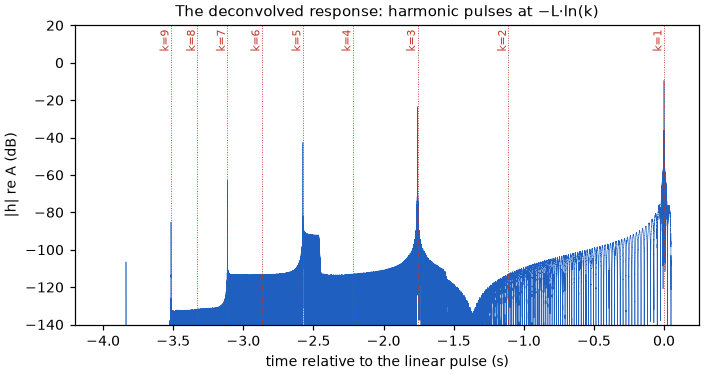
\includegraphics[width=0.95\linewidth]{hd-deconvolved.png}
  \caption{The deconvolved response of the worked example (a symmetric
  soft clipper), on a negative-delay axis. Odd orders carry content; the
  even orders' pulses are absent, as they must be for a symmetric
  device.}
  \label{fig:deconvolved}
\end{figure}

\item \textbf{Windowing.} Each order is cut out with a raised-cosine window
of half-widths $\ell_k$ (earlier in time, toward order $k+1$) and $r_k$
(toward order $k-1$), in samples:
\begin{equation}
  \begin{aligned}
  c &= \min\!\big(\tfrac{M}{2}-1,\ t_{\max} f_s\big),\qquad
  \ell_k = \Big\lfloor \min\!\big(c,\ \tfrac{(\Delta t_{k+1}-\Delta t_k) f_s}{2}\big)\Big\rfloor,\\
  r_k &= \begin{cases} \lfloor c \rfloor & k = 1\\
        \Big\lfloor \min\!\big(c,\ \tfrac{(\Delta t_k - \Delta t_{k-1}) f_s}{2}\big)\Big\rfloor & k > 1,\end{cases}
  \end{aligned}
  \label{eq:halfwidths}
\end{equation}
with $t_{\max}$ the half-width cap. The window is
$w(o) = \tfrac12(1 + \cos(\pi|o|/\ell_k))$ for $-\ell_k \le o < 0$ and
$\tfrac12(1 + \cos(\pi o/r_k))$ for $0 \le o < r_k$: unity at the pulse,
zero at each edge. An order is emitted only while $\ell_k \ge 16$ and
$r_k \ge 16$; the analyzer stops at the first order that fails, so a short
sweep simply carries fewer orders. The window duration
$T_k = (\ell_k + r_k)/f_s$ is what sets order $k$'s spectral resolution and
the correlation width the shaping predicate must clear.

\begin{figure}[htbp]
  \centering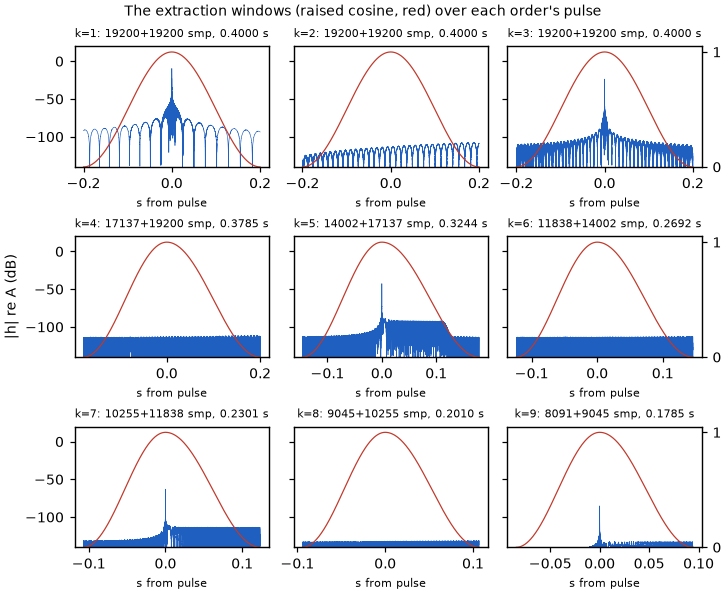
\includegraphics[width=0.95\linewidth]{hd-windows.png}
  \caption{The nine extraction windows over their pulses. Orders 1--3 take
  the full cap; from order 4 the gap to the neighbouring pulse binds.}
\end{figure}

\item \textbf{Spectra.} The windowed segment is placed with the pulse at
circular index 0 of an $M$-point buffer (so no linear-phase correction is
needed) and transformed:
\begin{equation}
  H_k[b] = \frac{1}{A}\,\mathrm{DFT}_M\{\,h[(p_k + o) \bmod N]\,w(o)\,\}[b],\qquad b = 0 \ldots M/2 ,
  \label{eq:Hk}
\end{equation}
with $p_k$ the pulse position. The $1/A$ is the \term{input-normalized}
convention: $H_1 = 1$ for a unit-gain linear device.

\item \textbf{Reading.} \label{sec:hd-reading} $H_k$ lives on the
\emph{output} frequency axis. The $k$-th harmonic of a fundamental $f_0$ is
read at $f = k f_0$, $|H_k|$ interpolated linearly between the two bins
adjacent to $f/(f_s/M)$, and reported as $20\log_{10}|H_k(k f_0)|$.

\item \textbf{Validity.} \label{sec:hd-validity} A read is trustworthy only
inside the \term{validity-bound}: $f_1 \le f_0 \le f_2$ and
\begin{equation}
  f_0 \le \frac{f_s}{2k+1},
  \label{eq:validity}
\end{equation}
beyond which the capture folds order $k+1$ onto the read at $k f_0$ (the
\term{alias-image} bound), and on a loopback-compensated record additionally
$f_0 \le f_{\mathrm{cal}}/k$ with $f_{\mathrm{cal}}$ the calibration sweep's
excited-band top. Invalid reads are excluded from every fit, feature,
summary and comparison.

\item \textbf{THD.} With the audible band $B$,
\begin{equation}
  \mathrm{THD}(f_0) = \frac{\sqrt{\sum_{k \ge 2,\ k f_0 \in B,\ \mathrm{valid}} |H_k(k f_0)|^2}}{|H_1(f_0)|},
  \label{eq:thd}
\end{equation}
THD and not THD+N; a point where the validity bound removed an in-band
order is flagged truncated. The curve is sampled on a log-spaced grid of
fundamentals from $1.5 f_1$ (the first fraction of the sweep is
fade-in territory) to $f_2$.
\end{enumerate}

\subsection{Read-time predicates on the result}
\label{sec:hd-predicates}
Three further judgements are computed from the stored spectra when a record
is displayed or compared; none is persisted, so fixing a predicate fixes every
stored record.

\paragraph{The floor.}\label{sec:hd-floor}
The rig's own floor comes from the embedded calibration's pooled THD-vs-
frequency stamp (one loopback sweep), read at $f_0$ by linear interpolation
on the $(\log f, \dB)$ plane, then adjusted: per track by $-10\log_{10}
N_{\mathrm{tracks}}$ (the pooled figure spread over the harmonic tracks),
for drive by the calibration sweep level minus the record's drive, and for
\term{averaging} by $-10\log_{10}(N/N_{\mathrm{cal}})$ --- applied only
where the residual the stamp measures is noise (inside the validity bound,
above the fade-in edge). A plugin record's operative floor enters as a
second, never-averaged bound and the applicable floor is the larger. A read
at or below its floor is a bound, not a figure.

\paragraph{Fundamental presence.} Every ratio to $H_1$ (THD above all) is
arithmetic unless the fundamental is a measurement: a fundamental sitting at
or beyond the analyzer's separation bound below the loudest valid, in-band
order is \term{fundamental-presence}-absent and nothing is divided by it.

\paragraph{Shaping.}\label{sec:hd-shaping}
Anything inside order $k$'s window is reported as $H_k$, the device's own
hiss included. Whether a read is content the circuit deterministically shaped
is decided by the \term{coherence} of the complex response along frequency:
with a lag of $\lceil \gamma/(T_k \cdot f_s/M) \rceil$ bins (clear of the
window's own spectral correlation) and $n$ samples,
\begin{equation}
  z_i = H(b_i + \mathrm{lag})\,\overline{H(b_i)},\qquad
  \Gamma = \frac{|\sum_i z_i|}{\sum_i |z_i|},
  \label{eq:coherence}
\end{equation}
which for pure noise is $1/\sqrt n$. $\Gamma$ maps to a signal-to-noise
ratio through a pinned Monte-Carlo table, that ratio to the read's own
1-$\sigma$ dB \term{scatter} (the Rician mean-of-dB
uncertainty~\citep{rice1944}), and a read is shaped when its ratio clears
the bar. The predicate's constants and both tables are in the parameter
table below.

\paragraph{Averaging.} $N$ back-to-back sweeps in one capture are analyzed
separately, each repeat \termas{derotation}{derotated} against the first by
one fitted delay for all orders (the delay $\delta$ maximizing
$\mathrm{Re}\sum z\,e^{j\omega\delta}$ over cross-spectral terms sampled per
order), and the complex spectra are averaged bin by bin. Magnitudes are
never averaged: $N$ reads of a biased quantity average to the same biased
number more precisely.

\subsection{Parameters}
\label{sec:hd-parameters}
Every value below is read from the manifest, which read it from the
shipped code. The per-order table follows.

% GENERATED by gen_docs.py from generated/manifest.json — do not edit
\begin{longtable}{@{}p{0.5\linewidth}p{0.45\linewidth}@{}}
\toprule Parameter & Value \\ \midrule \endhead
\multicolumn{2}{@{}l}{\textbf{Stimulus}} \\
start frequency $f_1$ & 20 Hz \\
end frequency $f_2$ & 10\,000 Hz \\
requested duration $\hat T$ & 10 s \\
sample rate $f_s$ & 96\,000 Hz \\
amplitude $A$ (re full scale) & 0.5 \\
rate constant $L$ & 1.6 s \\
synchronization cycles $f_1 L$ & 32 \\
actual duration $T = L\ln(f_2/f_1)$ & 9.943372957 s \\
sample count & 954\,564 \\
fade-in / fade-out & 0.05 s / 0.01 s \\
excited band (fade edges) & 20.635 Hz -- 9937.7 Hz \\
\multicolumn{2}{@{}l}{\textbf{Deconvolution}} \\
inverse-filter taper & 10 Hz -- 20 Hz \\
DFT length $N$ for one synth capture & 1\,048\,576 \\
\multicolumn{2}{@{}l}{\textbf{Extraction}} \\
harmonic count $K$ & 9 \\
response DFT length $M$ & 65\,536 \\
window half-width cap & 0.2 s \\
minimum half-width & 16 samples (a literal in the analyzer) \\
bin width $f_s/M$ & 1.4648438 Hz \\
bins per response & 32\,769 \\
\multicolumn{2}{@{}l}{\textbf{Grids}} \\
distance grid (\S 11) & 96 log-spaced points, 30--10\,000 Hz \\
THD curve grid & 127 of 128 requested, 30--9552.89 Hz \\
oracle grid (\texttt{synth}) & 48 points, 30--10\,000 Hz \\
distance fixed floor clamp & -80 dB \\
distance minimum resolved share & 0.2 \\
audible band & 20 Hz -- 20\,000 Hz \\
\multicolumn{2}{@{}l}{\textbf{Floor}} \\
calibration analyzed sweeps $N_{\mathrm{cal}}$ & 1 \\
averaging term at 1 / 2 / 4 / 8 sweeps & 0 dB / -3.01 dB / -6.021 dB / -9.031 dB \\
stamp read (median points) & 1 \\
at-floor epsilon & 0.1 dB \\
\multicolumn{2}{@{}l}{\textbf{Averaging}} \\
default / offered sweep counts & 4 / 1, 2, 4, 8 \\
pre-roll / gap / tail & 0.5 s / 0.5 s / 1 s \\
delay fit: samples per order & 48 \\
delay fit: scan limit / coarse / fine & $\pm$8 / 0.02 / 0.0005 samples \\
\multicolumn{2}{@{}l}{\textbf{Fundamental presence}} \\
analyzer separation bound & 76 dB \\
verdict grid points & 128 \\
\multicolumn{2}{@{}l}{\textbf{Shaping}} \\
window samples & 32 \\
pure-noise coherence $1/\sqrt{n}$ & 0.17678 \\
decorrelation factor & 2.4 \\
shaped SNR bar & 6 dB \\
unshaped scatter & 5.57 dB \\
\multicolumn{2}{@{}l}{\textbf{Summaries}} \\
lexicon version & 1.2.2 \\
\multicolumn{2}{@{}l}{\textbf{Oracle (\texttt{analysisdump synth})}} \\
post-sweep pad & 48\,000 samples \\
phantom Nyquist gate & 0.98 $\times f_s/2$ \\
ground-truth quadrature points & 262\,144 \\
noise generator increment & \texttt{0x9E3779B97F4A7C15} \\
\bottomrule
\end{longtable}


\begin{center}
% GENERATED by gen_docs.py from generated/manifest.json — do not edit
\begin{tabular}{@{}rrrrr@{}}
\toprule $k$ & $\Delta t_k = L\ln k$ (s) & window $T_k$ (s) & window (samples) & $\max f_0$ valid (Hz) \\ \midrule
1 & 0 & 0.4 & 38\,400 & 10\,000 \\
2 & 1.10904 & 0.4 & 38\,400 & 10\,000 \\
3 & 1.75778 & 0.4 & 38\,400 & 10\,000 \\
4 & 2.21807 & 0.37851 & 36\,337 & 10\,000 \\
5 & 2.5751 & 0.324365 & 31\,139 & 8727.27 \\
6 & 2.86682 & 0.269167 & 25\,840 & 7384.62 \\
7 & 3.11346 & 0.230135 & 22\,093 & 6\,400 \\
8 & 3.32711 & 0.201042 & 19\,300 & 5647.06 \\
9 & 3.51556 & 0.1785 & 17\,136 & 5052.63 \\
\bottomrule
\end{tabular}

\end{center}

\subsection{The result}
\begin{figure}[htbp]
  \centering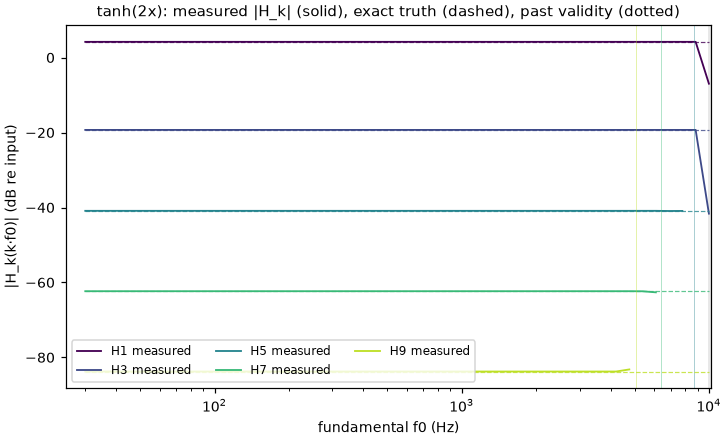
\includegraphics[width=0.95\linewidth]{hd-magnitude.png}
  \caption{The worked example, $y = \tanh(2x)$ at $A = 0.5$: measured
  $|H_k|$ for the odd orders against the exact Fourier amplitude of the
  nonlinearity at the sweep amplitude. Dotted segments lie past each order's
  validity bound; the shaded strip past the fade-out edge is the excited
  band's end, where the last grid point reads the ramp, not the device.}
  \label{fig:magnitude}
\end{figure}

The app's own rendering of the same measurement kind, from the user guide's
figure pipeline (a simulated device, rendered headlessly from the chart
views, never screenshotted):

\begin{figure}[htbp]
  \centering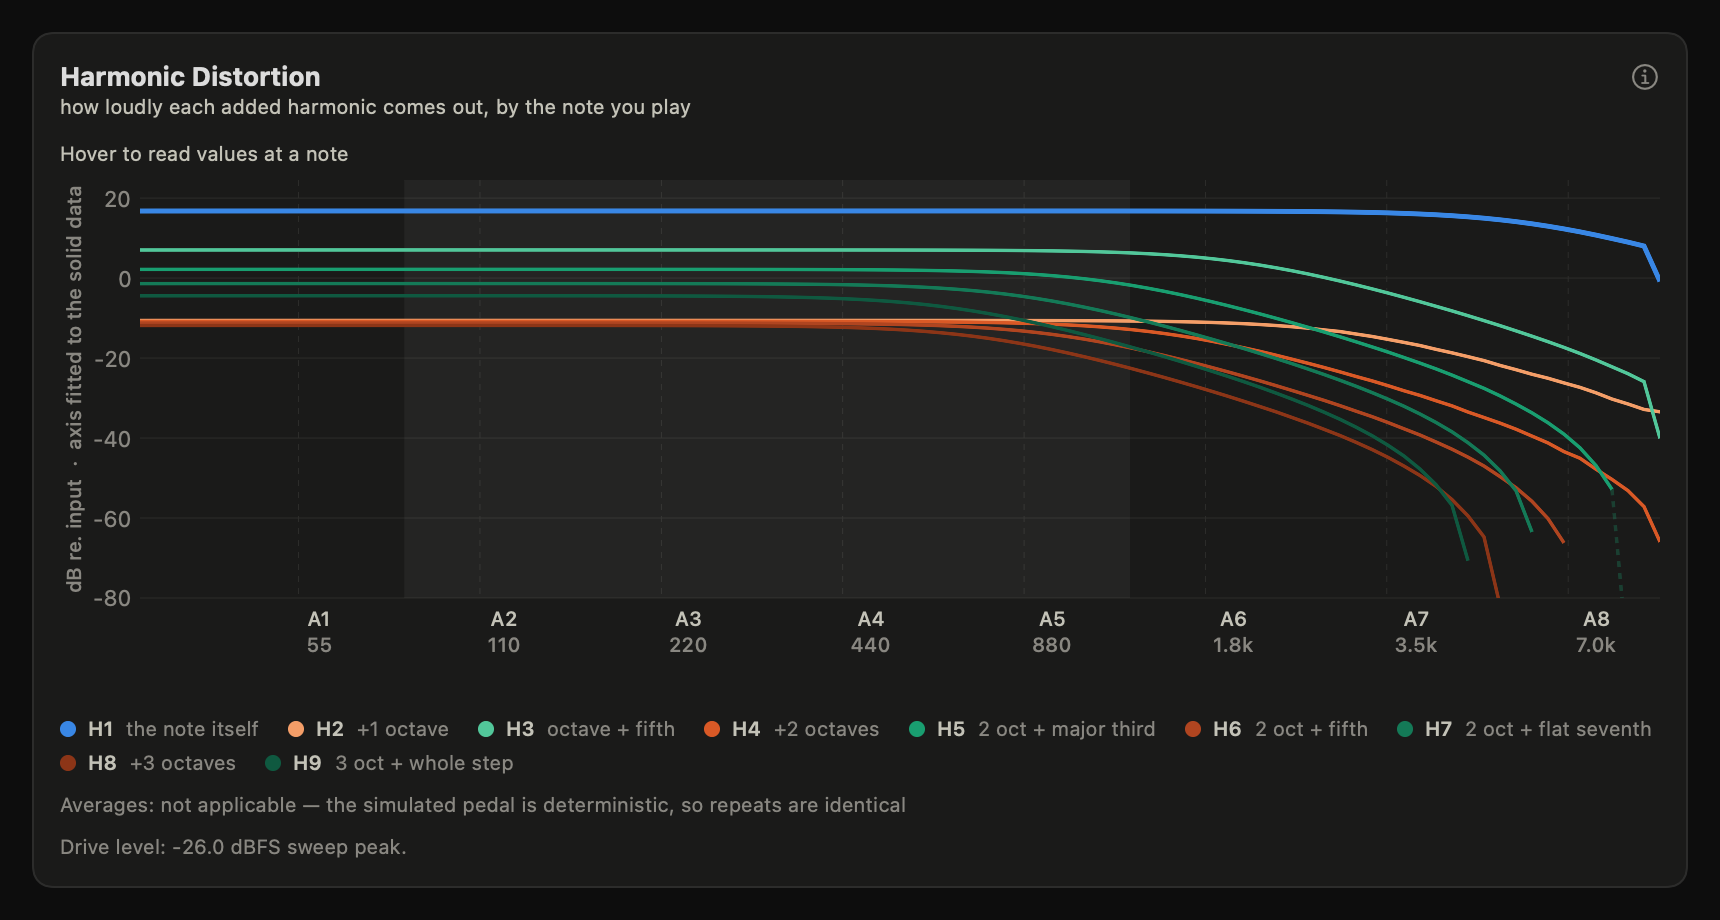
\includegraphics[width=0.85\linewidth]{harmonic-distortion--sim.png}\\[6pt]
  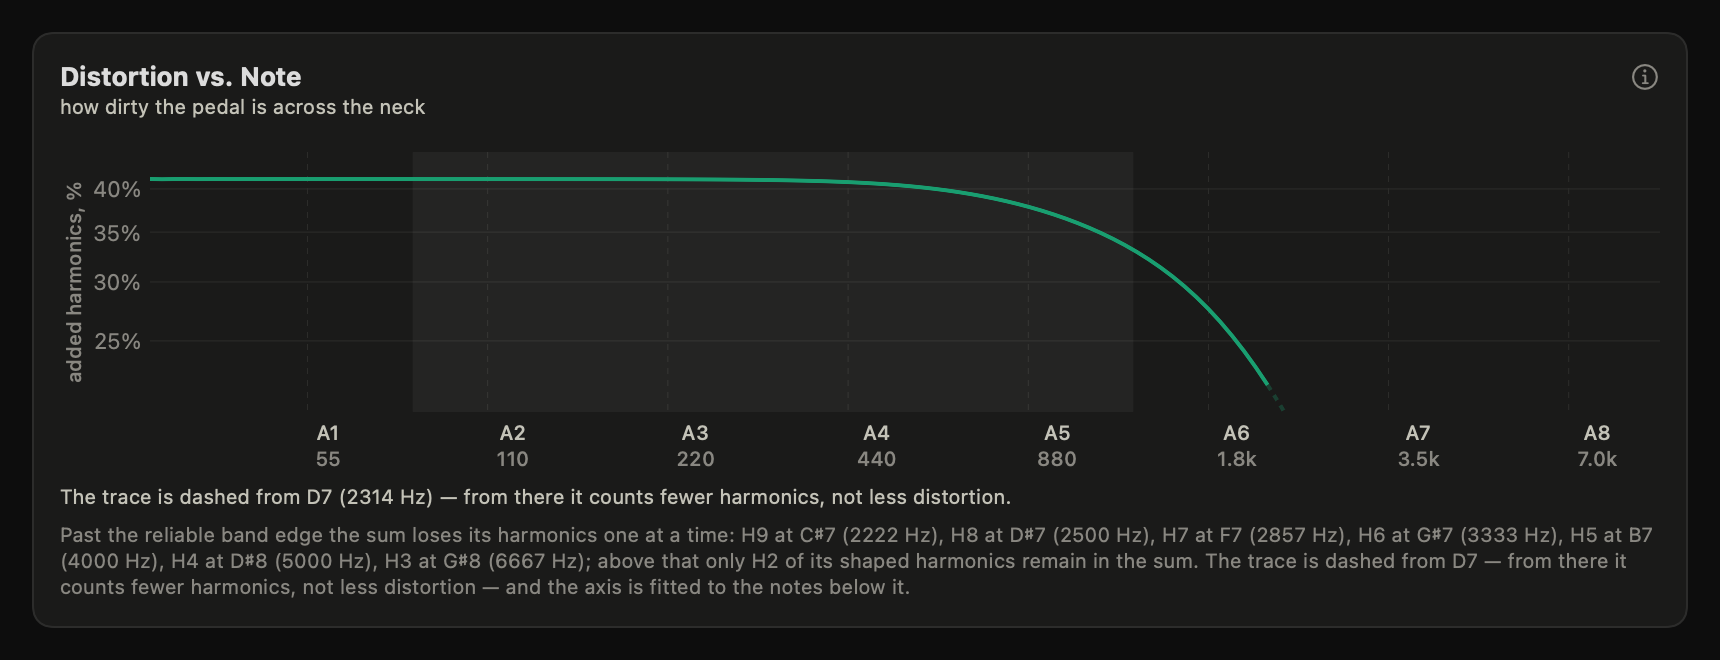
\includegraphics[width=0.85\linewidth]{harmonic-distortion--sim-thd.png}
  \caption{The Harmonic Distortion chart and the Distortion-vs-Note chart
  as the app draws them, from the guide's simulated fixture.}
\end{figure}

\subsection{Worked example and parity}
\label{sec:hd-example}
% GENERATED by gen_docs.py from a parity run (Swift vs Python vs analytic) — do not edit
\newcommand{\paritySwiftTolerance}{1e-08}
\newcommand{\parityAliasFreeTolerance}{0.01}
\newcommand{\parityPerSampleTolerances}{tanh 0.01 dB, poly 0.01 dB, hardclip 0.3 dB}
\newcommand{\parityEmptyDepth}{20}
\newcommand{\parityScatterMultiple}{3}
\newcommand{\parityTable}{
\begin{longtable}{@{}p{0.2\linewidth}rrrrrr@{}}
\toprule case & $k$ & expected & S$-$P & S$-$T band & P$-$T band & S$-$T full \\
 & & (dB) & (dB) & (dB) & (dB) & (dB) \\ \midrule \endhead
phantom & 1 & 0 & 3.9e-15 & 0.0052 & 0.0052 & 0.0052 \\
phantom & 2 & -10.458 & 5.3e-15 & 0.000851 & 0.000851 & 0.000851 \\
phantom & 3 & -20 & 1.1e-14 & 0.000121 & 0.000121 & 0.000121 \\
tanh & 1 & 4.2083 & 4.4e-15 & 0.00492 & 0.00492 & 0.00492 \\
tanh & 3 & -19.292 & 1.1e-14 & 0.000172 & 0.000172 & 0.000218 \\
tanh & 5 & -40.883 & 1.4e-13 & 4.17e-05 & 4.17e-05 & 0.0446 \\
tanh & 7 & -62.328 & 2.1e-12 & 4.29e-05 & 4.29e-05 & 0.299 \\
tanh & 9 & -83.757 & 2.1e-11 & 8.3e-05 & 8.3e-05 & 0.554 \\
tanh twin & 1 & 4.2083 & 3.6e-15 & 0.00515 & 0.00515 & 0.00515 \\
tanh twin & 3 & -19.292 & 1.4e-14 & 0.000169 & 0.000169 & 0.000169 \\
tanh twin & 5 & -40.883 & 1.4e-13 & 7.21e-05 & 7.21e-05 & 7.21e-05 \\
tanh twin & 7 & -62.328 & 1.6e-12 & 3.02e-05 & 3.02e-05 & 3.02e-05 \\
tanh twin & 9 & -83.757 & 1e-11 & 7.73e-05 & 7.73e-05 & 7.73e-05 \\
hardclip & 1 & -11.94 & 5.3e-15 & 0.0127 & 0.0127 & 0.0319 \\
hardclip & 3 & -21.955 & 7.1e-15 & 0.0896 & 0.0896 & 0.548 \\
hardclip & 5 & -27.372 & 1.4e-14 & 0.122 & 0.122 & 1.93 \\
hardclip & 7 & -31.859 & 1.4e-14 & 0.202 & 0.202 & 2.01 \\
hardclip & 9 & -36.348 & 1.4e-14 & 0.279 & 0.279 & 3.1 \\
hardclip twin & 1 & -11.94 & 7.1e-15 & 0.00515 & 0.00515 & 0.00515 \\
hardclip twin & 3 & -21.955 & 1.4e-14 & 0.000179 & 0.000179 & 0.000179 \\
hardclip twin & 5 & -27.372 & 1.1e-14 & 5.82e-05 & 5.82e-05 & 5.82e-05 \\
hardclip twin & 7 & -31.859 & 7.1e-15 & 2.04e-05 & 2.04e-05 & 2.04e-05 \\
hardclip twin & 9 & -36.348 & 2.1e-14 & 6.05e-05 & 6.05e-05 & 6.05e-05 \\
poly & 1 & 0.47533 & 3.7e-15 & 0.00523 & 0.00523 & 0.00523 \\
poly & 2 & -26.021 & 2.5e-14 & 0.000588 & 0.000588 & 0.000588 \\
poly & 3 & -34.54 & 4.3e-14 & 0.000136 & 0.000136 & 0.000136 \\
poly twin & 1 & 0.47533 & 3.7e-15 & 0.00516 & 0.00516 & 0.00516 \\
poly twin & 2 & -26.021 & 1.8e-14 & 0.00106 & 0.00106 & 0.00106 \\
poly twin & 3 & -34.54 & 5e-14 & 9.32e-05 & 9.32e-05 & 9.32e-05 \\
\bottomrule
\end{longtable}
}
\newcommand{\parityNoisyTable}{
\begin{tabular}{@{}rrrrrr@{}}
\toprule $k$ & expected (dB) & shaped points & S$-$P (dB) & S$-$T shaped, band (dB) & error / allowance \\ \midrule
1 & 4.2083 & 42 & 4.4e-15 & 0.00491 & 0.022 \\
3 & -19.292 & 42 & 1.1e-14 & 0.00246 & 0.036 \\
5 & -40.883 & 41 & 7.8e-14 & 0.0283 & 0.41 \\
7 & -62.328 & 38 & 8.7e-13 & 0.254 & 0.87 \\
9 & -83.757 & 36 & 1.2e-11 & 3.9 & 0.8 \\
\bottomrule
\end{tabular}
}
\newcommand{\parityTanhHone}{4.2083}
\newcommand{\parityTanhHthree}{-19.292}
\newcommand{\parityTanhHnine}{-83.757}
\newcommand{\parityTanhFullBand}{0.554}
\newcommand{\parityHardclipFullBand}{3.1}
\newcommand{\parityWorstSwift}{2.1e-11}


The \term{parity} runs four synthetic devices through both
implementations at one seed with no noise: a \term{phantom} of three orders
(exact by construction), $\tanh(2x)$, a hard clip at $\pm 0.1$ under an
amplitude of $0.5$, and $x + 0.2x^2 + 0.3x^3$. \machineFloorNote{} For
every valid point inside the excited band it asserts:
\begin{itemize}
  \item $|\text{Python} - \text{Swift}| \le \paritySwiftTolerance\dB$ on every
  order that carries content (measured maximum \parityWorstSwift\dB\ on
  this run; the two implementations differ only by DFT and transcendental
  rounding);
  \item both against analytic truth: $\le \parityAliasFreeTolerance\dB$ over
  the whole band for a phantom, and over the lower half of each order's
  validity band for the per-sample nonlinearities
  (\parityPerSampleTolerances);
  \item analytically empty orders read at least \parityEmptyDepth\dB\ below
  the case's loudest order on both sides, and the two sides agree on that
  residue.
\end{itemize}
The per-sample tolerances differ because the synthetic device, applied
sample by sample at $f_s$, aliases the content it generates above Nyquist
back into the band --- exactly as a simulated device in the app does, and
unlike a hardware device behind a converter's anti-alias filter. The
aliasing is worst in the top half-octave of each order's band: over the full
band, $\tanh(2x)$ departs from truth by up to \parityTanhFullBand\dB\ and the
hard clip (a near-square wave whose spectrum falls only as $1/k^2$) by up to
\parityHardclipFullBand\dB. That this is the synthetic device and not the
method is shown by each case's \emph{phantom twin}: the same first nine
Fourier amplitudes as an alias-free phantom, which the analyzer reads to
within \parityAliasFreeTolerance\dB\ over the whole band.

{\small\parityTable}

For $\tanh(2x)$ the exact amplitudes are $H_1 = \parityTanhHone\dB$,
$H_3 = \parityTanhHthree\dB$ and $H_9 = \parityTanhHnine\dB$ re input. A
fifth case adds seeded white noise at $-80\dB$FS and four averaged repeats
(the noise stream is reproduced exactly on both sides --- same generator,
same seeding). On the points the shipped predicate reads as shaped on both
sides, the error against truth must sit within \parityScatterMultiple\
times the read's own stated scatter; the last column is that ratio:

\begin{center}
\parityNoisyTable
\end{center}

\begin{figure}[htbp]
  \centering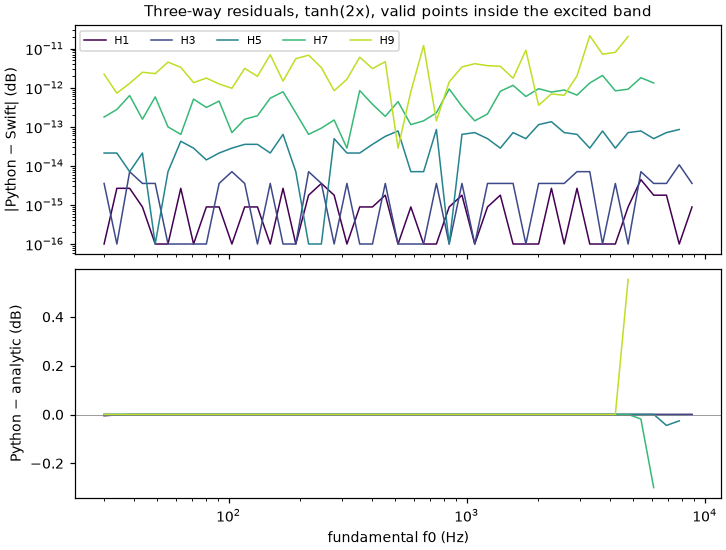
\includegraphics[width=0.95\linewidth]{hd-residuals.png}
  \caption{Three-way residuals for the worked example, every valid point
  inside the excited band. Top: $|\text{Python} - \text{Swift}|$, at the
  level of double-precision rounding. Bottom: Python minus analytic truth,
  showing the per-sample aliasing rising toward each order's band top.}
\end{figure}

\subsection{Limits and failure modes}
\begin{itemize}
  \item \textbf{The fade edges are measurement, not device.} The last grid
  point sits on $f_2$, inside the fade-out, and reads the ramp (the phantom's
  $H_1$ there is $11.7\dB$ low); on a compensated record the calibrated-band
  bound removes it, and on a raw or simulated one the \term{excited-band}
  is the honest limit. The first fraction of the sweep is treated the same
  way by every grid's $1.5 f_1$ start.
  \item \textbf{Leakage between orders is bounded, and the bound is
  measured.} An order's read is floored by what the loudest order leaks into
  its window: worst at the band's low edge, and the value the presence
  predicate uses is the measured one, posted a hair below what the analyzer
  demonstrated.
  \item \textbf{A read is not automatically content.} The shaping predicate
  exists because a symmetric device's even orders are a read of its noise;
  every quantity computed from an unshaped read describes the noise.
  \item \textbf{Aliasing in a simulated device.} A device applied per sample
  at $f_s$ folds its content above Nyquist into the band; the parity numbers
  above quantify it for two clippers. Hardware through a converter does not
  do this, and the alias-image bound~\eqref{eq:validity} is about the
  \emph{capture's} folding of the next order, a different mechanism.
  \item \textbf{Short sweeps carry fewer orders.} The 16-sample minimum
  half-width is a literal in the analyzer, pinned by the tool's guard rather
  than by the constants census; it binds only for sweeps far shorter than the
  standard plan.
  \item \textbf{The THD curve's top point.} The shipped curve requests 128
  log-spaced points but its top point can land an ulp above $f_2$ and be
  dropped by the band guard; the manifest reports the delivered count.
\end{itemize}


\section{Transfer Curve}
\label{sec:transfer}

\subsection{Purpose, and what the measurement cannot tell you}
The \term{transfer-curve} draws a device's clipping shape directly: while a
steady low-frequency sine plays, the instantaneous output is plotted against
the instantaneous input over one \term{averaged-cycle}. A memoryless device
retraces a single curve, the \term{static-curve}, and the figure's bends are
its \term{clipping}; anything that makes the output depend on where the
signal has just been --- a shifting bias point, stored charge --- opens the
figure into a loop. The result is the averaged cycle itself (two vectors of
$n$ phase bins), the static curve, and three dimensionless loop areas: the
total, the part a linear filter's phase rotation explains, and the part it
does not.

What it cannot tell you, stated once: (a) anything about other drive levels
--- one curve is one operating point, and a clipper whose knee sits above
the drive draws a straight line; (b) whether an open loop is memory or
filter phase --- ordinary tone filters rotate phase and open the loop
without any memory, which is why the \term{phase-removal} exists and why the
raw figure's middle band of loop area is hedged; (c) the device's
\emph{level} asymmetry once a series \term{coupling-capacitor} has removed
the output's mean, which every pedal's output stage does
(\S\ref{sec:transfer-limits}); (d) anything about a rig's own residual
alignment, which draws a loop the measurement cannot distinguish from the
device's (\S\ref{sec:transfer-limits}); and (e) anything about what the
distortion sounds like.

\subsection{The stimulus}
\label{sec:transfer-stimulus}
The stimulus is a sine at the probe note $f_0$ (the standard note is E2, at
the value the parameter table gives verbatim; other notes are exact
twelve-tone equal temperament with A4 $= 440$ Hz), at a linear peak
amplitude $A$:
\begin{equation}
  x[n] = A\,\sin\!\big(2\pi f_0\, n / f_s\big),\qquad n = 0 \ldots \lfloor T f_s\rfloor - 1,
  \label{eq:tone}
\end{equation}
scaled over its first and last $\lfloor t_{\mathrm{fade}} f_s\rfloor$ samples
by the raised cosine $\tfrac12(1 - \cos(\pi i / N_{\mathrm{fade}}))$, and
preceded and followed by silence (the pre-roll and the tail). The app plays
this stimulus, measures the loop latency per capture, and drops the pre-roll
before analysis; the oracle renders it through a synthetic device at zero
latency. The standard amplitude is the fingerprint sweep's drive
($-26$ dBFS), so the curve and the other measurement kinds describe one
operating point; the worked example below uses the loudest drive the
hardware sheet offers, because at the standard drive the reference clippers
draw a straight line, which is the point of the sheet's level control.

\subsection{The pipeline}
\label{sec:transfer-pipeline}
Given the tone $x[n]$ and the captured output $y[n]$, aligned by the
integer loop latency $\ell$:

\begin{enumerate}
\item \textbf{Phase binning.} With $P = f_s/f_0$ samples per cycle, every
sample $i \ge \lfloor s\,P \rfloor$ ($s$ the skipped opening cycles, while
the circuit settles) with $i + \ell$ inside the capture is assigned to the
bin
\begin{equation}
  b(i) = \min\!\Big(n - 1,\ \Big\lfloor n\cdot\big((i/P) \bmod 1\big)\Big\rfloor\Big),
  \label{eq:bin}
\end{equation}
and the averaged cycle is the per-bin mean of $x[i]$ and of $y[i + \ell]$
respectively: $\bar x_b$, $\bar y_b$, $b = 0 \ldots n-1$. Noise averages;
shape does not. Every sample to the end of the tone is binned, the fade-out
included --- only the start is skipped (\S\ref{sec:transfer-limits}).

\item \textbf{The box.} Every area is normalized by the rectangle that
bounds the figure (\term{box-normalization}):
\begin{equation}
  B = 4\,\max_b|\bar x_b|\,\max_b|\bar y_b| .
  \label{eq:box}
\end{equation}

\item \textbf{The total loop area.} The closed polyline
$(\bar x_b, \bar y_b)$ is split at every proper self-crossing and the
absolute shoelace areas of the resulting lobes are summed --- the
\term{lobe-area} --- so that opposite-winding lobes add instead of
cancelling (a signed integral sees only the fundamental's quadrature and
lets a figure-eight report zero). A lobe smaller than a fixed fraction of
its own polyline's box is dropped as bin noise. The reported figure is
$\mathrm{total} = \mathrm{lobes}(\bar x, \bar y)/B$.

\item \textbf{The fundamental ellipse.} Both cycles are projected onto
$\{1, \cos\theta_b, \sin\theta_b\}$, $\theta_b = 2\pi b/n$:
\begin{equation}
  a_x = \tfrac{2}{n}\sum_b \bar x_b \cos\theta_b,\quad
  b_x = \tfrac{2}{n}\sum_b \bar x_b \sin\theta_b,\quad
  a_y, b_y \text{ likewise},\quad
  \bar y = \tfrac{1}{n}\sum_b \bar y_b ,
  \label{eq:projection}
\end{equation}
and the fundamental-only trajectory is the least-squares
\term{fundamental-ellipse}, whose area is analytic:
\begin{equation}
  \mathrm{linear} = \frac{\pi\,|a_x b_y - a_y b_x|}{B} .
  \label{eq:linear}
\end{equation}
For an input $A\sin\theta$ and an output whose fundamental is
$R\sin(\theta + \varphi_1)$ this is $\pi A R\,|\sin\varphi_1| / B$ --- a
linear filter's rotation of the fundamental, never memory; for a linear
device, whose peak is its fundamental's, it reduces to
$(\pi/4)\,|\sin\varphi_1|$.

\item \textbf{The nonlinear residual.} The ellipse's output is subtracted
and the lobes of what remains are summed:
\begin{equation}
  \mathrm{nonlinear} = \frac{\mathrm{lobes}\big(\bar x,\ \bar y_b - \bar y - a_y\cos\theta_b - b_y\sin\theta_b\big)}{B} ,
  \label{eq:nonlinear}
\end{equation}
the \term{nonlinear-loop-area}: the harmonic content's own lobes, the
headline memory figure. A memoryless clipper's harmonics are in phase with
the drive and retrace; harmonics rotated by a filter, or by genuine memory,
enclose area here.

\item \textbf{The static curve.} The cycle is split at the bins of the
input's minimum and maximum into a rising branch and a falling one, each
reduced to a strictly ascending polyline in $\bar x$, interpolated linearly
onto a common grid of inputs from $\min\bar x$ to $\max\bar x$, and the two
interpolants are averaged --- per-branch resampling, never binning by input
value, whose sample density under a sinusoidal drive is $\propto
1/\sqrt{A^2 - x^2}$ and starves the centre.

\item \textbf{The memory verdict.} Taken on the nonlinear area (of the
compensated figure when the removal is accepted, \S\ref{sec:transfer-removal}):
below the first threshold the device reads memoryless-ish, above the second
it reads memory, and between them the reading is hedged deliberately ---
tone filtering \emph{ahead} of the clipper rotates every harmonic by $k$
times the drive's rotation, and a single fundamental cannot separate that
from mild memory. Both thresholds are literals in the shipped verdict; the
manifest reads them by bisecting it.
\end{enumerate}

Every derived quantity is recomputed from the stored cycle whenever a record
is read, so a stored record carries the cycle and nothing else that a fix
would have to migrate.

\subsection{Read-time predicates on the result}
\label{sec:transfer-predicates}
Three judgements are made against the record's paired Harmonic Distortion
analysis --- the same device, the same setting, the swept measurement of
\S\ref{sec:hd} --- when one exists; none is persisted.

\paragraph{Orientation.}
A plugin-path capture is aligned by correlation against the tone and can
land half a cycle off, which reverses the figure and, for an asymmetric
device, pairs $x(t)$ with $y(t + P/2)$. The \term{orientation} reads the
cycle's fundamental phase $\psi_1 = \angle Y[1] - \angle X[1]$ (direct DFTs
of the two cycles); when it sits within the lock tolerance of $\{0, \pi\}$
the capture is detectably locked, and when the paired $H_1$'s
\term{polarity} confidently disagrees with $\cos\psi_1 < 0$, the output
cycle is advanced by $n/2$ bins and the figure recomputed. Every other case
displays the figure as captured and implies nothing. Polarity itself is the
energy-weighted mean unit phasor of $H_1$ over the low band,
\begin{equation}
  m = \frac{\sum_b |H_1[b]|\,\mathrm{Re}\,H_1[b]}{\sum_b |H_1[b]|^2},\qquad
  \text{inverting} \Leftrightarrow m < 0,\quad \text{confidence} = |m| ,
  \label{eq:polarity}
\end{equation}
the real part and never the resultant length: a quadrature response is
coherent yet polarity-mute.

\paragraph{Fundamental presence.}
The memory verdict, the polarity statement and the pairing verdict all key
off a fundamental; the \term{fundamental-presence} reading is taken from
the paired record at $f_0$ (which separates orders far better than one
averaged cycle) and from the cycle's own DFT only when the paired reading is
undetermined. Where the fundamental is absent the page draws the raw figure
and states none of the three.

\paragraph{The phase removal.}
\label{sec:transfer-removal}
Harmonics generated \emph{behind} pre-clipper dispersion inherit
$k\,\varphi_{\mathrm{pre}}(f_0)$, while an $H_1$-based rotation would remove
$\varphi_{\mathrm{pre}}(k f_0)$; no single shift reconciles the two, so the
removal is fitted against the paired record's own branch phases
$\angle H_k(k f_0)$, which carry each harmonic's true burden
$k\,\varphi_{\mathrm{pre}}(f_0) + \varphi_{\mathrm{post}}(k f_0)$ by
construction. The steps:

\begin{enumerate}
\item \textbf{Fittable terms.} The cycle's harmonic phases are read from its
DFT, input-relative: $\mathrm{cyc}_k = \angle Y[k] - k\,\angle X[1]$. Order
$k$ votes when the paired record's \term{validity-bound} accepts $(k, f_0)$
and, for $k \ge 2$, both $|Y[k]|/|Y[1]|$ and $|H_k(k f_0)|/|H_1(f_0)|$
clear the magnitude floor; its weight is $w_k = \min(1, |Y[k]|/|Y[1]|)$
and its phase difference
\begin{equation}
  d_k = \mathrm{wrap}\big(\mathrm{cyc}_k - \angle H_k(k f_0) - \gamma_k\big),\qquad
  \gamma_k = \mathrm{wrap}\big((k-1)\,\pi/2\big),
  \label{eq:diff}
\end{equation}
$\gamma_k$ being the Novák factor between the cycle's convention and the
deconvolver's. Fewer than the minimum number of terms means insufficient
evidence, never a verdict.

\item \textbf{The frame fit.} The two captures each measured their own
latency, so a shift between their frames is legitimate and must never be
applied as rotation. One shift $\Delta l$ (samples) is fitted by maximizing
the weighted phase coherence
\begin{equation}
  C(\Delta l) = \sum_k w_k \cos\!\big(d_k - k\,\omega_0\,\Delta l\big),\qquad
  \omega_0 = 2\pi f_0 / f_s ,
  \label{eq:framefit}
\end{equation}
by a coarse scan over $\pm P/2$ and a fine scan around its maximum (both
steps are literals, stated in the parameter table): the \term{frame-fit}.
The residuals $r_k = \mathrm{wrap}(d_k - k\omega_0\Delta l)$ give the
\term{pairing-residual}, the weighted RMS over $k \ge 2$ (the fundamental
can always be absorbed into $\Delta l$, so consistency lives in the
harmonics); above the tolerance the outcome is a pairing mismatch.

\item \textbf{The anchored sequential fold.} The frame-mapped branch phase
$m_k = \mathrm{cyc}_k - r_k$ is what the paired record predicts for harmonic
$k$ in the cycle's own frame. Its burden over the memoryless
\term{lattice} $\{0, \pi\}$ is known only modulo $\pi$ (the multiple
removed is the device's own harmonic sign, which the figure keeps), and the
folds must come out mutually consistent. The fundamental is anchored: its
lattice point is $\pi$ when the paired polarity reads inverting and $0$
when not (the nearest point only when polarity is not confident, and then
the sign is quotable only inside the lattice-sign confidence), giving
$e_1 = \mathrm{wrap}(m_1 - \sigma_1)$. Each higher voting order, in
ascending order, folds against a trend: $k\,e_1$ for the first, and for
every later one $a\,k + F(k)$, where $F(k) = \phi^{u}_1(k) - \phi^{u}_1(1) +
(e_1 - \omega_0\Delta l)$ is the paired $H_1$'s unwrapped phase \emph{shape}
anchored at the fundamental's burden (the post-clipper term) and the slope
$a$ is refit after each fold over the orders already folded (the pre-clipper
term; the fundamental never votes in it):
\begin{equation}
  \beta_k = m_k - \pi\,\mathrm{round}\!\Big(\frac{m_k - \mathrm{trend}_k}{\pi}\Big),\qquad
  a = \frac{\sum_{j \le k} w_j\, j\,(\beta_j - F(j))}{\sum_{j \le k} w_j\, j^2} .
  \label{eq:fold}
\end{equation}
The per-order assumption is that the curvature beyond the ramp is under
$\pi/2$ --- true of the resistor--capacitor networks pedals are built from,
and weakest at the lowest order, where it holds across every device class
measured.

\item \textbf{The all-pass.} The correction is a smooth function of
frequency, applied to every bin of the cycle's spectrum at unity
magnitude: the deviations $\beta_k - a k - F(k)$ at the voting orders are
interpolated by a shape-preserving cubic (Fritsch--Carlson, constant beyond
the end nodes), and for $1 \le k < n/2$
\begin{equation}
  Y[k] \leftarrow Y[k]\,e^{-j\theta_k},\qquad
  \theta_k = a k + F(k) + \mathrm{dev}(k),
  \label{eq:allpass}
\end{equation}
with DC and the real Nyquist bin untouched. The compensated cycle is the
inverse real DFT and the figure is recomputed from it. Content above the
voting orders survives phase-corrected rather than being resynthesized
away, which is what removed the truncation ripple an earlier per-order
resynthesis drew on hard-clipped plateaus. The correction is
\emph{measured} up to the support $k_{\max} f_0$, the highest voting order
times the drive note; above it the ramp is extended, $F$ follows $H_1$'s
phase as far as its grid holds a value, and the deviation holds its last
knot --- an extrapolation the page's caption states.

\item \textbf{The outcome.} One of five: compensated; a pairing mismatch (no
shift reconciles the harmonic phases); insufficient evidence (too few
fittable terms); a negligible raw loop (the total under the dead zone,
decided after the fit ran so polarity still rides it, and outranking a
mismatch --- a noise-dominated tiny loop must not wear a warning); and a
tripped metric guard, when a removal that passed the residual still grew a
\emph{decomposed} area beyond its tolerance (the unsigned total is never
compared: the ellipse and the harmonic lobes partially cancel in it). A
pairing mismatch has two possible causes the residual alone does not
separate: a session mismatch --- another setting or another time, resolved
by re-measuring both kinds together --- and a structural one, a device
whose harmonics have no fundamental-anchored phase relationship (a
frequency doubler), which no re-measurement resolves.

\item \textbf{Polarity, confirmed.} The figure states polarity only when a
fit ran, its residual confirms the pairing, and the fundamental's lattice
sign resolved; the robust $H_1$ statistic supplies the sign, the fit the
trust. Absence is honest; a guessed sign is not.
\end{enumerate}

An older correction --- rotating harmonic $k$ by $\angle H_1(k f_0)$ alone
--- remains in the kernel with no consumer, and is not the method this
document describes.

\subsection{Parameters}
\label{sec:transfer-parameters}
Every value below is read from the manifest, which read it from the shipped
code; the two verdict thresholds were located by bisecting the shipped
verdict, and the scan steps, the bin count, the grid, the polarity band and
the analyzer's unused default are literals the manifest carries as rule
strings.

% GENERATED by gen_docs.py from generated/manifest.json — do not edit
\begin{longtable}{@{}p{0.5\linewidth}p{0.45\linewidth}@{}}
\toprule Parameter & Value \\ \midrule \endhead
\multicolumn{2}{@{}l}{\textbf{Stimulus}} \\
standard note / frequency $f_0$ & E2 / 82.4 Hz \\
standard amplitude $A$ (re full scale) & 0.05 (-26.02 dBFS) \\
tone duration $T$ / pre-roll / tail & 1.5 s / 0.2 s / 0.2 s \\
fade-in and fade-out $t_{\mathrm{fade}}$ & 0.02 s \\
skipped cycles (the app's call) & 8 (the analyzer's own default is 5, unused) \\
sample rate $f_s$ (the manifest's) & 96\,000 Hz \\
samples per cycle $P$ at $f_0$ & 1165.0485 \\
probe notes offered & E2, A2, E3, A3, E4, A4, E5, A5, A6, C7 \\
note-range capture & E2, A3, A4 \\
drive level bounds (hardware / plugin ceiling) & -60 to -6 dBFS / 0 dBFS \\
\multicolumn{2}{@{}l}{\textbf{Binning and the figure}} \\
phase bins $n$ & 256 \\
static-curve grid points & 101 \\
lobe floor (fraction of the box) & 0.0002 \\
\multicolumn{2}{@{}l}{\textbf{Memory verdict (bisected from the shipped verdict)}} \\
memoryless-ish below & 0.05 \\
memory effects from & 0.15 \\
\multicolumn{2}{@{}l}{\textbf{Phase removal (\S\,6.5)}} \\
dead zone $\varepsilon$ (raw total area) & 0.01 \\
pairing residual tolerance & 0.25 rad \\
fit magnitude floor (both sides) & 0.005 (-46 dB) \\
minimum fittable terms & 3 \\
lattice sign confidence & 0.6 rad \\
metric-guard tolerance (decomposed areas) & 0.02 \\
frame-fit scan: coarse / fine step & 0.05 / 0.001 samples (literals) \\
\multicolumn{2}{@{}l}{\textbf{Orientation and polarity}} \\
half-cycle lock tolerance & 0.05 rad \\
polarity confidence threshold & 0.35 \\
polarity band & 20 Hz -- 2 kHz (literals) \\
\multicolumn{2}{@{}l}{\textbf{Fundamental presence}} \\
analyzer separation bound & 76 dB \\
\multicolumn{2}{@{}l}{\textbf{Oracle (\texttt{analysisdump transfer-synth})}} \\
biquad default $Q$ & 0.70710678 \\
truth series orders $K$ & 200 \\
truth quadrature points & 262\,144 \\
\bottomrule
\end{longtable}


\subsection{The result}
\begin{figure}[htbp]
  \centering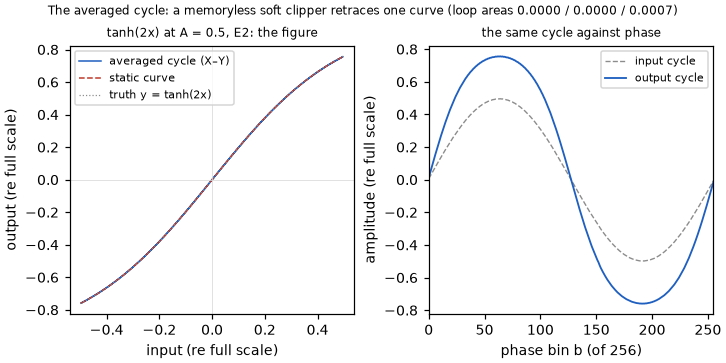
\includegraphics[width=0.95\linewidth]{transfer-cycle.png}
  \caption{The worked example, $y = \tanh(2x)$ at $A = 0.5$ and E2, no
  filter: the averaged cycle as the X--Y figure with the static curve and
  the exact curve overlaid (left; the three coincide), and the same cycle
  against phase (right). Every loop area is zero to the bin floor.}
  \label{fig:transfer-cycle}
\end{figure}

\begin{figure}[htbp]
  \centering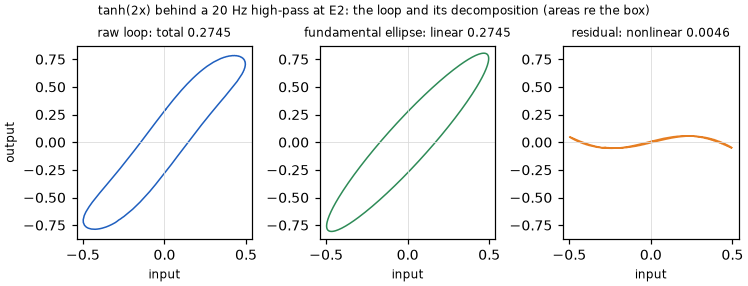
\includegraphics[width=0.95\linewidth]{transfer-loop-decomposition.png}
  \caption{The same clipper behind a 20 Hz second-order high-pass at E2:
  the raw loop, the fitted fundamental ellipse and the residual after the
  ellipse's output is subtracted, each with its normalized area. The filter
  draws the ellipse; the residual holds only the harmonics' own rotation.}
  \label{fig:transfer-decomposition}
\end{figure}

\begin{figure}[htbp]
  \centering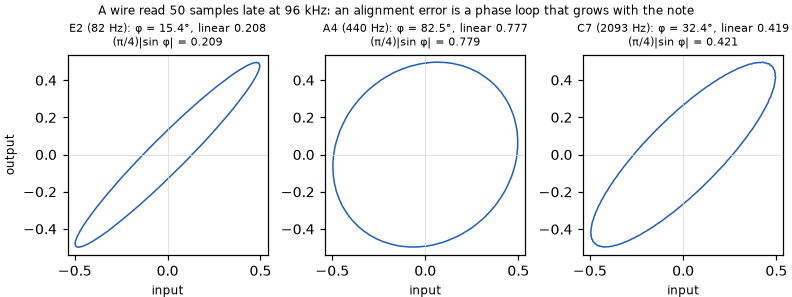
\includegraphics[width=0.95\linewidth]{transfer-delay-loop.png}
  \caption{A wire, analyzed 50 samples late at 96 kHz, at three notes: an
  alignment error is a phase loop that grows with the note. Each title
  gives the phase the error implies at that note, the measured linear area
  and its closed form $(\pi/4)|\sin\varphi|$.}
  \label{fig:transfer-delay}
\end{figure}

\begin{figure}[htbp]
  \centering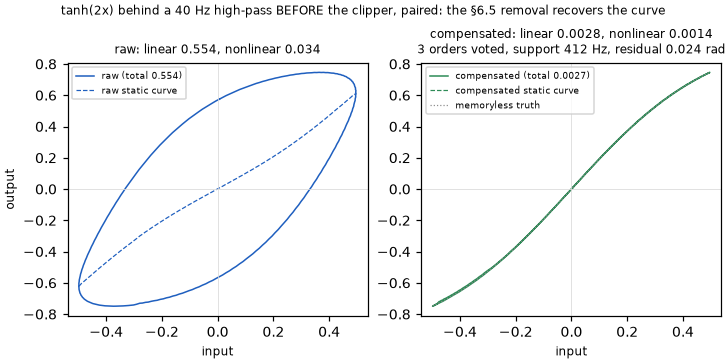
\includegraphics[width=0.95\linewidth]{transfer-compensation.png}
  \caption{The soft clipper behind a 40 Hz high-pass placed \emph{before}
  the clipper --- the pre-dispersive case an $H_1$-only rotation cannot
  handle --- paired with its own swept analysis. Left: the raw figure and
  its static curve. Right: the compensated figure over the memoryless truth,
  with the orders that voted, the support and the residual.}
  \label{fig:transfer-compensation}
\end{figure}

\begin{figure}[htbp]
  \centering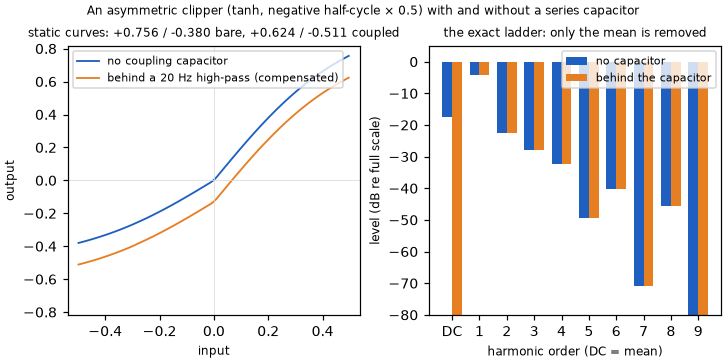
\includegraphics[width=0.95\linewidth]{transfer-coupling.png}
  \caption{An asymmetric clipper (the negative half-cycle scaled by one
  half) with and without a series capacitor: the static curve's unequal
  clip levels are centred by the capacitor while the exact harmonic ladder
  loses only its mean --- the even harmonics survive.}
  \label{fig:transfer-coupling}
\end{figure}

The app's own rendering of the same measurement kind, from the user guide's
figure pipeline (a simulated device, rendered headlessly from the chart
view with the removal on):

\begin{figure}[htbp]
  \centering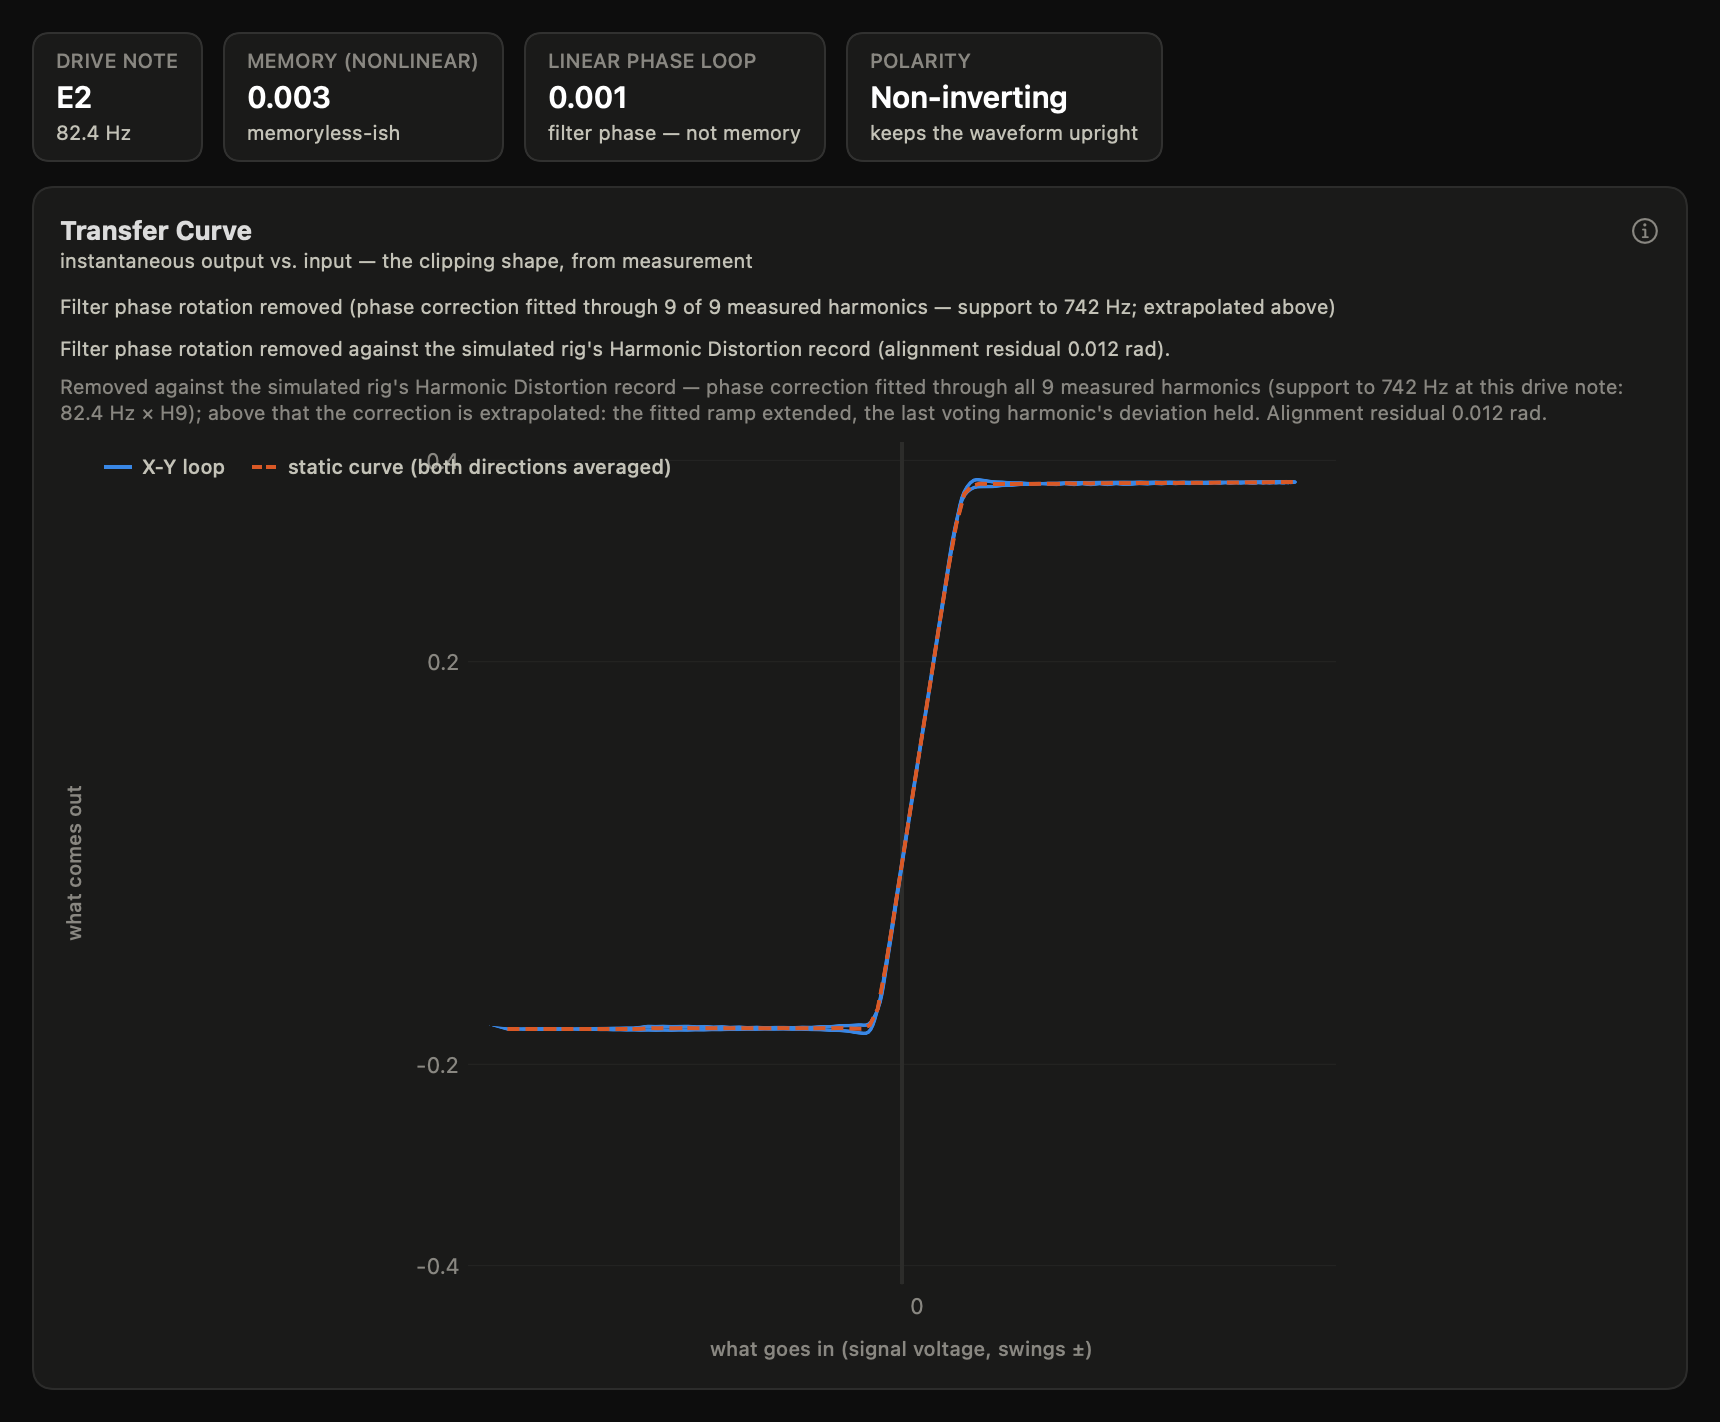
\includegraphics[width=0.85\linewidth]{transfer-curve--sim-compensated.png}
  \caption{The Transfer Curve view as the app draws it, from the guide's
  simulated fixture, with the phase removal applied and its caption stating
  the support and the residual.}
\end{figure}

\subsection{Worked example and parity}
\label{sec:transfer-example}
% GENERATED by gen_docs.py from a parity run (Swift vs Python vs closed-form truth) — do not edit
\newcommand{\tparitySwift}{1e-09}
\newcommand{\tparitySwiftShift}{1e-09}
\newcommand{\tparityEllipseRatio}{0.01}
\newcommand{\tparityEllipseRatioLong}{0.001}
\newcommand{\tparityCompStatic}{0.01}
\newcommand{\tparityCompCycle}{0.02}
\newcommand{\tparityFrameShift}{0.5}
\newcommand{\tparityResidual}{0.05}
\newcommand{\tparityCompArea}{0.005}
\newcommand{\tparityMemorylessNonlinear}{0.005}
\newcommand{\tparityRawStaticSmooth}{0.01}
\newcommand{\tparityRawStaticHardclip}{0.05}
\newcommand{\tparityRawStaticEllipse}{0.05}
\newcommand{\tparityCaseCount}{21}
\newcommand{\tparityWorstSwift}{$\le$\,1e-10}
\newcommand{\tparityWorstShift}{$\le$\,1e-10}
\newcommand{\tparityEllipseTable}{
\begin{tabular}{@{}lrrrrr@{}}
\toprule case & $f_0$ (Hz) & $\varphi_1$ ($^\circ$) & measured & $(\pi/4)|\sin\varphi_1|$ & ratio \\ \midrule
b-lp-E2 & 82.4 & -4.3 & 0.0586 & 0.058997 & 0.99327 \\
b-lp-A6 & 1\,760 & -100.2 & 0.77136 & 0.7729 & 0.998 \\
b-lp-C7 & 2093 & -113.4 & 0.71634 & 0.72094 & 0.99362 \\
c-delay-E2 & 82.4 & 15.5 & 0.20771 & 0.20923 & 0.99275 \\
c-delay-A4 & 440 & 82.5 & 0.77706 & 0.77868 & 0.99792 \\
c-delay-C7 & 2093 & 32.4 & 0.41926 & 0.42128 & 0.9952 \\
b-lp-E2-15s & 82.4 & -4.3 & 0.058976 & 0.058997 & 0.99965 \\
b-lp-A6-15s & 1\,760 & -100.2 & 0.77283 & 0.7729 & 0.9999 \\
b-lp-C7-15s & 2093 & -113.4 & 0.72058 & 0.72094 & 0.9995 \\
\bottomrule
\end{tabular}
}
\newcommand{\tparityMemorylessTable}{
\begin{tabular}{@{}lrrrrr@{}}
\toprule case & $A$ & total & linear & nonlinear & static vs truth (of peak) \\ \midrule
a-tanh & 0.5 & $\le$\,1e-10 & 5.95e-06 & 0.000719 & 0.00298 \\
a-tanh-plan & 0.05 & $\le$\,1e-10 & 4.52e-08 & 0.000612 & 4.41e-05 \\
a-hardclip & 0.5 & 0.00132 & 9.68e-05 & 0.00196 & 0.0266 \\
a-asym & 0.5 & $\le$\,1e-10 & 0.000119 & 0.000458 & 0.00337 \\
a-param & 0.5 & $\le$\,1e-10 & 1.41e-05 & 0.000939 & 0.00747 \\
\bottomrule
\end{tabular}
}
\newcommand{\tparityPairedTable}{
\begin{tabular}{@{}llrrrrrrr@{}}
\toprule case & class & voted & support & residual & $\Delta l$ & comp.\ lin. & comp.\ nonlin. & comp.\ vs truth \\
 & & & (Hz) & (rad) & (samples) & & & (of peak) \\ \midrule
d-tanh-lp & compensated & 3 & 412 & 0.00322 & -0.172 & 0.00049 & 0.00054 & 0.0044 \\
d-tanh-hp & compensated & 3 & 412 & 0.00945 & -0.388 & 0.00024 & 0.00066 & 0.0022 \\
e-tanh-prehp & compensated & 3 & 412 & 0.0237 & -0.272 & 0.0028 & 0.0014 & 0.004 \\
f-asym-hp & compensated & 7 & 659.2 & 0.0108 & -0.102 & 0.0015 & 0.0008 & 0.0055 \\
g-tanh-inv-lp & compensated & 3 & 412 & 0.00322 & -0.172 & 0.00049 & 0.00054 & 0.0044 \\
g-tanh-shift & negligible loop & 3 & 412 & 0.00833 & 0.401 & -- & -- & -- \\
g-tanh-paired & negligible loop & 3 & 412 & 0.00816 & -0.0763 & -- & -- & -- \\
\bottomrule
\end{tabular}
}
\newcommand{\tparityEllipseDeficitShort}{0.73}
\newcommand{\tparityEllipseDeficitLong}{0.05}
\newcommand{\tparityAsixRatio}{0.998}
\newcommand{\tparityAsixRatioLong}{0.9999}
\newcommand{\tparityEtwoRatio}{0.9933}
\newcommand{\tparityEtwoRatioLong}{0.99965}
\newcommand{\tparityWorstFrameShift}{0.39}
\newcommand{\tparityWorstResidual}{0.0237}
\newcommand{\tparityWorstCompStatic}{0.0055}
\newcommand{\tparityWorstCompArea}{0.0028}
\newcommand{\tparityWorstMemorylessNonlinear}{0.002}
\newcommand{\tparityHardclipStatic}{0.027}
\newcommand{\tparityTanhStatic}{0.003}
\newcommand{\tparityTanhPlanStatic}{4.4e-05}
\newcommand{\tparityTanhPlanNonlinear}{0.00061}
\newcommand{\tparityPrehpRawNonlinear}{0.0343}
\newcommand{\tparityPrehpCompNonlinear}{0.0014}
\newcommand{\tparityAsymRawNonlinear}{0.015}
\newcommand{\tparityAsymVoted}{7}
\newcommand{\tparityTanhVoted}{3}
\newcommand{\tparityShiftPsi}{3.144}
\newcommand{\tparityShiftLatticeDistance}{0.0026}
\newcommand{\tparityRemovalStatus}{The removal's parity is established: every paired filtered case compensates on both sides and the two implementations agree on the compensated figure to the Swift-vs-Python tolerance.}


The \term{parity} runs \tparityCaseCount\ synthetic cases through both
implementations, each a known device --- one of the reference
nonlinearities between an optional pre-filter and an optional post-filter,
each a second-order (Butterworth) low-pass or high-pass --- driven by the
plan's own tone and, where paired, measured by the swept method of
\S\ref{sec:hd} for its reference. Beside every measured quantity the
oracle prints a truth computed by quadrature: for a memoryless device with
no filter the curve $y(x)$ itself; otherwise the Fourier series of the
clipper's output at the pre-filter's delivered drive, each order scaled and
rotated by the post-filter's analytic response and by any planted
alignment error, and --- for the compensated figure --- the same series
with every phase returned to the lattice and every magnitude kept.
\machineFloorNote{} The test asserts:
{\sloppy
\begin{itemize}
  \item Swift against Python: every cycle value, static-curve value,
  compensated value, area, $\psi_1$, residual and fit term within
  \tparitySwift\ (measured maximum \tparityWorstSwift\ on this run), the
  frame shift within \tparitySwiftShift\ samples (measured
  \tparityWorstShift), and every discrete reading --- class, flip,
  polarity, tile, verdict, presence --- identical;
  \item the fundamental ellipse against its closed form
  $(\pi/4)\,|\sin\varphi_1|$ on a linear device: a ratio within
  \tparityEllipseRatio\ of one at the plan's tone (measured deficit at
  worst \tparityEllipseDeficitShort\,\%) and within
  \tparityEllipseRatioLong\ at ten times its length (measured
  \tparityEllipseDeficitLong\,\%);
  \item the raw static curve against the truth, as a fraction of the
  output peak: \tparityRawStaticSmooth\ for smooth memoryless devices
  (measured \tparityTanhStatic\ on the soft clipper, \tparityTanhPlanStatic\
  at the standard drive), \tparityRawStaticHardclip\ for the hard clip
  (measured \tparityHardclipStatic: a 256-bin cycle rounds a corner by
  about an eighth of a bin's input span), \tparityRawStaticEllipse\ for an
  open ellipse (the branch-mean curve of an open loop is least trustworthy
  where the branches meet); and a memoryless device's nonlinear area under
  \tparityMemorylessNonlinear\ (measured \tparityWorstMemorylessNonlinear);
  \item every paired filtered device compensates, finds the planted frame
  shift within \tparityFrameShift\ samples (measured \tparityWorstFrameShift),
  keeps its residual under \tparityResidual\ rad (measured
  \tparityWorstResidual), recovers the memoryless truth to
  \tparityCompStatic\ of peak on the static curve (measured
  \tparityWorstCompStatic) and \tparityCompCycle\ on the cycle, and reads
  both compensated areas under \tparityCompArea\ (measured
  \tparityWorstCompArea).
\end{itemize}
\par}
\tparityRemovalStatus

The memoryless cases, at the loudest hardware drive and (one case) the
standard drive, where the soft clipper is within its linear region:

\begin{center}\small\tparityMemorylessTable\end{center}

The linear devices --- the identity behind the low-pass at three notes and
under a 50-sample alignment error at three notes --- at the plan's tone and
at ten times its length:

\begin{center}\small\tparityEllipseTable\end{center}

The paired cases: two post-filters and the pre-filter on the soft clipper,
the asymmetric clipper behind a DC-blocking high-pass, an inverted device,
the half-cycle lock and the unfiltered clipper (whose raw loop is under the
dead zone, so the removal is a no-op and the fit still confirms polarity):

\begin{center}\scriptsize\setlength{\tabcolsep}{4pt}\tparityPairedTable\end{center}

Two readings from those tables are worth stating in words. The
pre-dispersive case's raw nonlinear area, \tparityPrehpRawNonlinear, sits in
the hedged band of the verdict with no memory in the device at all, and the
removal takes it to \tparityPrehpCompNonlinear\ --- the mid-band hedge in
the pipeline is exactly this case. And the half-cycle lock is undone: the
captured $\psi_1$ read \tparityShiftPsi\ rad, \tparityShiftLatticeDistance\
from the lattice, the paired polarity read non-inverting, and the resolved
figure ascends.

\subsection{Limits and failure modes}
\label{sec:transfer-limits}
{\sloppy
\begin{itemize}
  \item \textbf{The normalization is the box's, and the constant is
  $\pi/4$ only for a linear device.} The ellipse area is $\pi A R
  |\sin\varphi_1| / (4 A\,y_{\max})$; on a clipped output the peak is not
  the fundamental's and the figure is $(\pi/4)(R/y_{\max})|\sin\varphi_1|$,
  which can exceed $(\pi/4)|\sin\varphi_1|$ (a square wave's fundamental is
  $4/\pi$ of its peak). A reader converting a linear-device figure to an
  angle uses $\varphi_1 = \arcsin(4\,\mathrm{linear}/\pi)$. On the
  synthetic single-pole check the shipped code reads the closed form to
  \tparityEllipseDeficitShort\,\% at the plan's tone and
  \tparityEllipseDeficitLong\,\% at ten times its length, so a deficit of
  several percent on a hardware capture is in the measurement chain, not in
  the metric's constant.
  \item \textbf{The fade-out is binned.} The skipped opening cycles protect
  the start; every sample to the end of the tone is binned, the last
  $t_{\mathrm{fade}}$ under its ramp, a phase-dependent weighting whose
  share of the average falls with the tone's length. It is the whole of the
  deficit above (the E2 ratio moves from \tparityEtwoRatio\ to
  \tparityEtwoRatioLong\ between the two lengths), and it lowers the
  captured input peak by a few tenths of a percent at the plan's length.
  \item \textbf{A residual alignment error is a loop.} An
  \term{alignment-error} of $e$ samples rotates the fundamental by
  $\varphi = 2\pi f_0 e / f_s$ and draws a linear area of
  $(\pi/4)|\sin\varphi|$ on a wire --- growing with the note
  (Figure~\ref{fig:transfer-delay}). The integer latency the app removes
  leaves at least the fractional part, and a rig can leave more; on a
  device, that loop is indistinguishable from the device's own linear-phase
  loop. Two notes measured on one rig let a reader test the hypothesis:
  a single $e$ must reproduce both deficits. The nonlinear area is untouched
  by it on a linear device.
  \item \textbf{The coupling capacitor removes level asymmetry, not
  harmonic asymmetry.} A clipper clamped at $+a$ and $-b$ at roughly equal
  duty carries a mean near $(a - b)/2$; a series capacitor at the output
  strips it, leaving levels of $\pm(a+b)/2$ --- equal magnitudes from an
  unequal circuit (Figure~\ref{fig:transfer-coupling}). The shape asymmetry
  remains, and the even harmonics in the paired swept analysis are where
  the asymmetry is read. Because every pedal has one, a transfer curve
  essentially never shows the raw asymmetry of an asymmetric clipper.
  \item \textbf{The support ends at the highest voting order.} A harmonic
  too quiet to clear the magnitude floor on either side does not vote
  (the soft clipper at this drive seats \tparityTanhVoted\ orders, the
  asymmetric clipper \tparityAsymVoted); above the support the correction is
  the extended ramp, the $H_1$ shape and a held deviation, and a hard-clipped
  device has content far above it.
  \item \textbf{The branch phase is read at the nearest bin.} The paired
  record's phase at $k f_0$ is the nearest bin's, so a read can be off by
  up to half a bin width times the filter's phase slope, which the frame fit
  absorbs as a fictitious shift of a fraction of a sample (measured up to
  \tparityWorstFrameShift\ samples on the parity cases) and leaves in the
  higher orders' residuals.
  \item \textbf{The bins round a corner.} With $n$ bins per cycle a hard
  clip's corner is averaged over a bin's input span, and the static curve
  departs from the exact curve there by a few percent of the clip level;
  the smooth devices read under one percent of peak.
  \item \textbf{The static curve of an open loop.} The branch-mean estimate
  is least trustworthy where the two branches meet, at the input's
  extremes; on a wide ellipse it departs from the true line by a few
  percent of peak there. The app draws the static curve dashed on every
  figure; on an open loop its ends are where the estimate is least
  trustworthy.
  \item \textbf{A declined removal names its class, not its cause.} The
  residual separates a genuine pairing from a mismatch; it does not separate
  a session mismatch from a structural one, and the two need different
  remedies (\S\ref{sec:transfer-removal}).
\end{itemize}
\par}

\clearpage
\section{Compression}
\label{sec:compression}
% The parity fragment defines macros the stimulus and predicate sections
% quote before the worked example prints its tables, so it is input here.
% GENERATED by gen_docs.py from a parity run (Swift vs Python vs the closed-form ladder) — do not edit
\newcommand{\cparitySwiftTolerance}{1e-07}
\newcommand{\cparitySwiftFilteredTolerance}{1e-06}
\newcommand{\cparitySwiftTruthTolerance}{1e-06}
\newcommand{\cparityEmptyDepth}{140}
\newcommand{\cparityHOne}{1e-06}
\newcommand{\cparityTruthSmooth}{0.0002}
\newcommand{\cparityTruthKinked}{0.0002}
\newcommand{\cparityTruthFiltered}{0.005}
\newcommand{\cparityTHD}{0.0001}
\newcommand{\cparityFade}{0.02}
\newcommand{\cparityKnee}{0.1}
\newcommand{\cparityCleanup}{0.001}
\newcommand{\cparityStamp}{0.02}
\newcommand{\cparityGain}{1e-09}
\newcommand{\cparityLatency}{1e-09}
\newcommand{\cparityMiscut}{1e-06}
\newcommand{\cparitySeparationOverBar}{60}
\newcommand{\cparityCaseCount}{24}
\newcommand{\cparitySeparationBar}{76}
\newcommand{\cparityTwinCount}{2}
\newcommand{\cparityMiscutSamples}{1}
\newcommand{\cparityWorstSwift}{3.1e-08}
\newcommand{\cparityWorstSwiftFiltered}{1.6e-08}
\newcommand{\cparityWorstSwiftTruth}{3.3e-07}
\newcommand{\cparityLeakageTable}{
\begin{tabular}{@{}rrrrrrrrr@{}}
\toprule bin distance & 1 & 2 & 3 & 4 & 5 & 6 & 7 & 8 \\ \midrule
leakage (dB re the tone) & -158.2 & -171.8 & -180.2 & -186.4 & -191.4 & -195.5 & -199.1 & -202.2 \\
\bottomrule
\end{tabular}
}
\newcommand{\cparityLeakageOne}{-158.2}
\newcommand{\cparityLeakageTwo}{-171.8}
\newcommand{\cparityLeakageEight}{-202.2}
\newcommand{\cparityFadeLeakageOne}{-109.7}
\newcommand{\cparityDeviceTable}{
\begin{tabular}{@{}lrrrrrrrr@{}}
\toprule case & content & S$-$P (dB) & $H_1$ (dB) & raw (dB) & at & residue (dB) & THD residue & fade (dB) \\ \midrule
a-tanh8 & 71 & 2e-10 & 3e-08 & 0.042 & step 0 h3 & 5.8e-05 & $\le$\,1e-10 & -0.0031 \\
a-tanh8-twin & 71 & 2.6e-10 & 3e-08 & 0.042 & step 0 h3 & 5.8e-05 & $\le$\,1e-10 & -0.0057 \\
a-tanh2 & 47 & 1e-09 & 3e-08 & 0.212 & step 3 h3 & 6.9e-05 & $\le$\,1e-10 & -0.0054 \\
c-hardclip & 16 & $\le$\,1e-10 & 9e-07 & 8.22e-05 & step 34 h9 & 8.2e-05 & 7.8e-06 & -0.0017 \\
c-hardclip-twin & 16 & $\le$\,1e-10 & 3e-08 & 9.73e-07 & step 33 h5 & 1.2e-07 & 3.7e-09 & -0.0057 \\
l-tanh-prehp & 71 & 1.6e-08 & 2.6e-08 & 0.0416 & step 0 h3 & 1.2e-08 & $\le$\,1e-10 & -0.00295 \\
l-poly-postlp & 63 & 1.5e-08 & 2.9e-08 & 0.21 & step 7 h3 & 0.0018 & $\le$\,1e-10 & -0.00558 \\
\bottomrule
\end{tabular}
}
\newcommand{\cparityReadTimeTable}{
\begin{tabular}{@{}llllr@{}}
\toprule case & knee & cleanup & floor source & S$-$P (dB) \\ \midrule
a-tanh8 & -22 dBFS & cleans up at -27.17 dBFS & none & 2e-10 \\
a-tanh8-twin & -22 dBFS & cleans up at -27.17 dBFS & none & 2.6e-10 \\
a-tanh2 & none & cleans up at -15.13 dBFS & none & 1e-09 \\
a-linear & none & always clean & none & $\le$\,1e-10 \\
b-identity-noise & none & always clean & capture noise & $\le$\,1e-10 \\
b-identity-null & none & always clean & capture noise & $\le$\,1e-10 \\
b-identity-null-loop & none & always clean & null run & $\le$\,1e-10 \\
b-tanh8-null-loop & -22 dBFS & cleans up at -26.88 dBFS & null run & $\le$\,1e-10 \\
c-hardclip & -19.2 dBFS & cleans up at -20.03 dBFS & none & $\le$\,1e-10 \\
c-hardclip-twin & -19.2 dBFS & cleans up at -20.03 dBFS & none & $\le$\,1e-10 \\
d-subunity-break & ≤ -70 dBFS & cleans up at -30.18 dBFS & none & $\le$\,1e-10 \\
d-subunity-line & none & cleans up at -50 dBFS & none & $\le$\,1e-10 \\
d-hardclip-zone & ≤ -70 dBFS & cleans up at -68.06 dBFS & none & $\le$\,1e-10 \\
d-hardclip-under & ≤ -70 dBFS & never clean & none & $\le$\,1e-10 \\
e-fine & -19.2 dBFS & cleans up at -19.77 dBFS & none & $\le$\,1e-10 \\
f-plugin & -18.5 dBFS & cleans up at -20.14 dBFS & none & $\le$\,1e-10 \\
g-gain0 & -22 dBFS & cleans up at -27.17 dBFS & capture noise & $\le$\,1e-10 \\
g-gain12 & -22 dBFS & cleans up at -27.17 dBFS & capture noise & 1.3e-10 \\
h-latency & -22 dBFS & cleans up at -27.17 dBFS & none & 2e-10 \\
h-miscut & none & always clean & none & $\le$\,1e-10 \\
i-operative & -22 dBFS & cleans up at -27.17 dBFS & stated floor & $\le$\,1e-10 \\
j-absent & not\_stated & none & none & $\le$\,1e-10 \\
j-separation & not\_stated & none & none & 3.1e-08 \\
k-simulation & -21.2 dBFS & cleans up at -27.14 dBFS & none & 4.6e-10 \\
l-tanh-prehp & -22 dBFS & cleans up at -27.17 dBFS & none & 1.6e-08 \\
l-poly-postlp & none & cleans up at -20 dBFS & none & 1.5e-08 \\
\bottomrule
\end{tabular}
}
\newcommand{\cparityWorkedContent}{71}
\newcommand{\cparityWorkedHOne}{3e-08}
\newcommand{\cparityWorkedRaw}{0.042}
\newcommand{\cparityWorkedRawAt}{step 0 h3}
\newcommand{\cparityWorkedResidue}{5.8e-05}
\newcommand{\cparityWorkedResidueAt}{step 28 h9 (74 dB clear)}
\newcommand{\cparityWorkedTHDResidue}{$\le$\,1e-10}
\newcommand{\cparityWorkedFade}{-0.0031}
\newcommand{\cparityWorkedKnee}{-22.469}
\newcommand{\cparityWorkedKneeResolution}{0.748}
\newcommand{\cparityWorkedKneeLabel}{-22 dBFS}
\newcommand{\cparityWorkedPreSlope}{0.9936}
\newcommand{\cparityWorkedPostSlope}{0.5749}
\newcommand{\cparityWorkedTruthKnee}{-22.469}
\newcommand{\cparityWorkedKneeError}{$\le$\,1e-10}
\newcommand{\cparityWorkedCleanup}{-27.175}
\newcommand{\cparityWorkedTruthCleanup}{-27.175}
\newcommand{\cparityWorkedCleanupError}{1.3e-06}
\newcommand{\cparityWorkedSharpness}{0.586}
\newcommand{\cparityWorkedAsymptote}{0.478}
\newcommand{\cparityWorstFade}{-0.0057}
\newcommand{\cparityLeastFade}{-0.0017}
\newcommand{\cparityWorstResidueSmooth}{6.9e-05}
\newcommand{\cparityWorstResidueKinked}{8.2e-05}
\newcommand{\cparityWorstResiduePhantom}{5.8e-05}
\newcommand{\cparityWorstResidueFiltered}{0.0018}
\newcommand{\cparityWorstTHDResidue}{7.8e-06}
\newcommand{\cparityWorstHOne}{9e-07}
\newcommand{\cparityWorstKnee}{0.0534}
\newcommand{\cparityWorstCleanup}{0.00034}
\newcommand{\cparityClipOnset}{-20}
\newcommand{\cparityClipKnee}{-19.16}
\newcommand{\cparityClipKneeAboveOnset}{0.842}
\newcommand{\cparityClipPostSlope}{0.157}
\newcommand{\cparityClipResolution}{0.0534}
\newcommand{\cparityStampError}{0.00744}
\newcommand{\cparityGainShift}{$\le$\,1e-10}
\newcommand{\cparityGainKneeMove}{$\le$\,1e-10}
\newcommand{\cparityLatencyFound}{100}
\newcommand{\cparityLatencyMove}{$\le$\,1e-10}
\newcommand{\cparityMiscutMove}{3e-08}
\newcommand{\cparitySeparation}{158.2}
\newcommand{\cparityAbsentDepth}{79.97}
\newcommand{\cparityAbsentFraction}{0.833}
\newcommand{\cparitySimulationKnee}{-21.19}
\newcommand{\cparitySimulationKneeResolution}{0.388}
\newcommand{\cparitySimulationKneeGap}{1.28}
\newcommand{\cparityFineDelivered}{52}
\newcommand{\cparityFineKnee}{-19.21}
\newcommand{\cparityFineKneeResolution}{0.0534}
\newcommand{\cparityFineKneeMove}{0.0534}
\newcommand{\cparityLineMeasuredKnee}{none}
\newcommand{\cparityLineTruthKnee}{≤ -70 dBFS}
\newcommand{\cparityLineTruthPreSlope}{0.85}
\newcommand{\cparityBreakKnee}{≤ -70 dBFS}
\newcommand{\cparityBreakPreSlope}{0.85}
\newcommand{\cparityBreakPostSlope}{0.2}
\newcommand{\cparityPartBStatus}{Part B's parity is established: on every read-time case — the identity through noise with and without a null run, the null run through a loop with its own distortion, the exact sub-unity lines, the clippers at and under the floor, the fine window, the plugin window, the stated floor, and the device with no fundamental — the two implementations agree on every bound, every class, every run, every knee field, every cleanup state and level, every floor label and every verdict.}


\subsection{Purpose, and what the measurement cannot tell you}
A \term{compression-curve} --- the app's ``touch response'' --- is one
tone at the probe note stepped through a \term{probe-grid} of input levels
from quiet to loud, and at each step the output level of the
\term{fundamental} and the \term{thd} at that note, read on one snapped
window by a \term{one-bin-estimator}. It answers what the sweep of
\S\ref{sec:hd} cannot: where, as the drive rises, one decibel in stops
being one decibel out --- the \term{knee} of a \term{hinge-fit} through
the whole curve, a point with a \term{resolution-band} or a bound at the
floor --- and where, going down, the distortion falls under a threshold
(the \term{cleanup-reading}). This instrument is NOT the sweep. There is no
deconvolution and no extraction window; the estimator is its own
(\S\ref{sec:compression-pipeline}), and the chapter owns its equation.

What it cannot tell you, stated once: (a) anything at a note other than
the probe note --- a circuit whose tone stack sits ahead of its clipper
compresses differently across the neck, and one curve is one pitch;
(b) anything between two steps --- the knee is interpolated by a fit
whose breakpoint is free to land between rungs, but the fit is a summary
of the measured points and a feature narrower than a rung is ambiguous
(the \term{fine-window} exists for that); (c) anything about a knee the
grid did not reach --- a device already compressing at the quietest step
has its knee somewhere below it, and the answer is a bound, never a
number; (d) what a THD read near its floor is --- the \term{noise-bound}
says where the read is the rig, and the \term{floor-class} says so per
point; (e) the second crossing --- the cleanup level is the FIRST
crossing from the quiet end, and a device whose THD rises, falls and
rises again with drive (\S\ref{sec:journey}'s level-trend law: THD is not
monotone in drive for a soft-knee overdrive) is quoted at its first
crossing only; and (f) anything about what the distortion sounds like.

\subsection{The stimulus}
\label{sec:compression-stimulus}
The grid is $N$ levels evenly spaced in dB from a floor to a ceiling
inclusive,
\begin{equation}
  \ell_i = \ell_{\min} + (\ell_{\max} - \ell_{\min})\,\frac{i}{N - 1},
  \qquad A_i = 10^{\ell_i/20},
  \label{eq:probegrid}
\end{equation}
with an optional fine window merged in: a span $[l, h]$ clamped inside
the grid, filled at the fine spacing with its count capped (so a wide
window widens its own spacing rather than growing the run), each fine
level appended unless a level already sits within a tenth of the fine
step of it, and the whole list sorted --- so the fine points interleave
the lattice. Two drive windows exist, the hardware one anchored to gain
staging (the ceiling is the loudest drive that cannot clip the converter;
the floor keeps a stated clearance over a staged rig's converter floor and
reaches below the old floor so that high-gain knees resolve to points) and
the plugin one reaching digital full scale (the parameter table gives
both). The floor, the ceiling, the step count and the window are the
user's per run, so a record's grid is read from its own points and never
assumed.

The \term{stepped-tone} is one sine at the probe note $f_0$ whose
amplitude walks the grid quiet to loud, the phase continuous across
steps:
\begin{equation}
  x[n] = A[n]\,\sin\!\big(2\pi f_0 n / f_s\big),\qquad
  A[n] = \begin{cases}
    A_{i-1} + (A_i - A_{i-1})\,\tfrac12\big(1 - \cos(\pi\, m/R)\big) & m < R \\
    A_i & \text{otherwise,}
  \end{cases}
  \label{eq:steppedtone}
\end{equation}
$n$ the global sample index, $m$ the index within step $i$, $R$ the ramp
length in samples ($A_{-1} = 0$). Each step is a \term{settle-window}: a
settle region of $S$ samples, whose first $R$ carry the raised-cosine
ramp from the previous amplitude and whose remainder lets the device
settle unread, then a measurement window of $M$ samples. $M$ is the
\term{cycle-snap}: the requested measurement duration rounded to a whole
number of periods of $f_0$ (at least four), so the window holds an
integer number of cycles of the fundamental and of every
\term{harmonic-order}, and the estimator sees no leakage from the tone
itself. The last $R$ samples of the whole tone fade to zero over a
raised cosine --- and that fade lies INSIDE the last step's measurement
window, a fact with a consequence \S\ref{sec:compression-limits} states.

\paragraph{The assembly, and a mirror.} The measurement of record plays a
pre-roll of silence, the tone and a tail of silence; the pre-roll's rms
is the \term{noise-stamp}, a per-capture measurement of the loop PLUS the
device's own hiss; the analyzer is handed the pre-roll plus the embedded
calibration's round-trip latency as its cut. That assembly is not a
MeasureKit type: it lives in the app's measurement service (the record's
path), by copy in the command-line tool, differently in Simulation Mode
(the tone alone --- no pre-roll, no stamp, latency zero, its quality's
shorter windows and fewer steps; the parameter table gives both
qualities) and again in the plugin probe (a development tool). The
oracle behind this chapter reproduces the app's assembly once and states
it as a mirror, because there is no shipped function to call; a
\code{CompressionPlan} in the kernel is the filed follow-up
(\S\ref{sec:compression-limits}). Nothing capture-time moved for this
chapter.

\subsection{The pipeline}
\label{sec:compression-pipeline}
Given the captured output $y[n]$, the latency $\ell$ (the pre-roll plus
the calibration's measured round trip; on the plugin path the pre-roll
alone, since that path measures and removes its latency per capture) and
the stamp $\sigma$:
{\sloppy
\begin{enumerate}
\item \textbf{The window.} Step $i$'s window is
$y[iS' + S + \ell \;\ldots\; iS' + S + \ell + M)$, $S' = S + M$ the
samples per step; a window that runs before the capture's start or past
its end is skipped, silently.

\item \textbf{The gate.} The window's rms $r_i = \sqrt{\sum y^2 / M}$;
with a stamp, a step with $r_i \le \sigma\,10^{g/20}$ --- within the
stated margin $g$ of the capture's own hiss --- is the \term{noise-gate}'s:
excluded from the curve and counted. Its ``output level'' would be the
hiss, not the tone, and would flatten the quiet end into a phantom knee;
the quietest surviving step is then the effective floor, and a bound
reads from it.

\item \textbf{The estimator.} The amplitude of one frequency $f$ in the
window, by a Hann-windowed one-bin DFT with the window's coherent gain
compensated:
\begin{equation}
  a(f) = \frac{2\,\big|\sum_{m=0}^{M-1} y[m]\,w[m]\,e^{-j\,2\pi f m/f_s}\big|}{\sum_m w[m]},
  \qquad w[m] = \tfrac12\big(1 - \cos(2\pi m/(M-1))\big),
  \label{eq:hann}
\end{equation}
$m$ the window-local index (only the magnitude is read). On the snapped
window a pure tone reads its amplitude to rounding; what the Hann buys
is robustness to what the snap does not cover --- the ramp's tail and a
latency cut that is slightly wrong --- and \S\ref{sec:compression-example}
measures both. A window of eight samples or fewer reads zero.

\item \textbf{The point.} $a_1 = a(f_0)$ is the output amplitude. For
$k = 2 \ldots K$ in order: if $k f_0$ reaches $0.95$ of Nyquist or
exceeds the band's top the loop ENDS (every higher order is excluded);
if it sits under the band's bottom the order is skipped; else $a_k =
a(k f_0)$ joins the sum. Then
\begin{equation}
  \mathrm{thd}_i = \frac{\sqrt{\sum_k a_k^2}}{a_1},
  \label{eq:cthd}
\end{equation}
a ratio of AMPLITUDES over the declared audible band (THD, not THD+N);
zero when the fundamental reads zero. At the default note every rate the
app offers sums $k = 2\ldots K$ entirely; the band's top cuts in above
$f_0 = 20\,000/K$ Hz. The point carries $A_i$, $a_1$, $r_i$ and
$\mathrm{thd}_i$; its levels are $20\log_{10}$ of them (with a small
literal guard against a zero fundamental) and its gain is their
difference.

\item \textbf{The curve.} The points sort ascending by input amplitude
(a fine window's points interleave the lattice), and the stored curve is
the note, the rate, the points, and --- as additive fields --- the stamp
and the gate's count. Nothing derived is stored: the knee, the cleanup
and the classes are computed when the record is read, so a fixed
estimator retroactively fixes every stored record.
\end{enumerate}
\par}

\subsection{Read-time predicates on the result}
\label{sec:compression-predicates}
Everything below is computed from the frozen curve when a record is read.

\paragraph{The incremental slopes.} Between consecutive points, the
\term{incremental-slope} $s_i = \Delta\mathrm{out}_i / \Delta\mathrm{in}_i$
in dB per dB (1 when the input step is not positive): 1 is clean, 0 a
hard limit.

\paragraph{The hinge fit, in four verdicts.}
With $x_i$ and $y_i$ the input and output levels in dB over $n \ge 4$
points, the \term{hinge-fit} is
\begin{equation}
  y = c_0 + c_1 x + c_2 \max(0, x - k),
  \label{eq:hinge}
\end{equation}
two lines meeting continuously at a breakpoint $k$; $s_1 = c_1$ is the
pre-knee slope and $s_2 = c_1 + c_2$ the post-knee slope. The breakpoint
is swept over a fine set of candidates between the second and the
third-from-last probe (both segments keep at least two points), each
candidate solved by the normal equations of the columns $[1, x,
\max(0, x-k)]$ with a small ridge on the diagonal, and the candidate with
the smallest error wins; the whole $(k, \mathrm{SSE})$ profile is kept.
Against it stands the single-line fit with its own error
$\mathrm{SSE}_{\mathrm{lin}}$ and slope $s_{\mathrm{lin}}$. Two constants
govern: the post-knee threshold $\tau_s$ (a knee compresses when
$s_2 < \tau_s$) and the pre-knee unity tolerance $\delta$; the probe step
$p = x_1 - x_0$ is the LOCAL first rung --- on every uniform stored grid
it equals the average step exactly, and on a mixed grid with a fine
window mid-ladder the average would understate the spacing at the floor.
The verdict, in order:
\begin{enumerate}
  \item \emph{No break.} If the best hinge does not beat the line by the
  stated factor, the curve is ONE line: clean throughout when
  $s_{\mathrm{lin}} \ge 1 - \delta$ (no knee), else sub-unity throughout
  --- a BOUND at $x_0$ with resolution $p$ and both slopes
  $s_{\mathrm{lin}}$ (mild compression everywhere, the knee at or below
  the floor).
  \item \emph{Never compresses.} A break exists but $s_2 \ge \tau_s$: no
  knee.
  \item \emph{The \term{unity-guard}.} $s_1 < 1 - \delta$: a BOUND at
  $x_0$ with resolution $p$ and the fitted slopes. The device is already
  compressing at the quietest probe, no clean segment anchors the fit,
  and the fitted corner is an artifact of a curve bent everywhere; the
  guard is against UNITY, not against the compression threshold ---
  compared against $\tau_s$, every slope between the two passed as a
  confident point, which is how a drive-max soft-knee overdrive record in
  the library once reported a false point. The bound carries its fitted
  pre-knee slope as the evidence the page quotes.
  \item \emph{The \term{bound-zone}.} $k \le x_0 + p$: a BOUND at $k$
  with resolution $p$ --- a breakpoint within one probe step of the floor
  cannot be anchored from below.
\end{enumerate}
Otherwise a POINT at $k$, whose \term{resolution-band} is the interval of
candidates whose error stays within five percent of the best; half its
width is the resolution, never finer than the candidate spacing, and it
sets the decimals the level is displayed with. A bound's label reads
``$\le$''.

\paragraph{The cleanup reading.} The first point already at or above the
threshold $\tau$ is \emph{never clean}; else the first $i$ with
$\mathrm{thd}_i \ge \tau$ gives \emph{cleans up} at the interpolated
crossing (the same linear interpolation and literal guard as the Gain
Map's \eqref{eq:crossing}); else the
raw function returns the top of the probed range, which the
\term{cleanup-reading} reclassifies as \emph{always clean} --- the edge
of the probe is never dressed up as a property of the device. Only a
genuine crossing quotes a level or draws a marker.

\paragraph{The floor, from three sources.}
The first source is the \term{noise-bound}: the stamp expressed as a
worst-case THD at each point,
\begin{equation}
  F_{\sigma,i} = \frac{\sqrt2\,\sigma}{a_{1,i}},
  \label{eq:noisebound}
\end{equation}
because if every bit of the broadband noise power landed in the harmonic
bins the THD numerator would read exactly $\sqrt2\,\sigma$ --- a strict
upper bound on what noise alone can contribute, conservative in the
refuse-to-call-noise-distortion direction, and one that climbs toward the
quiet end as the fundamental shrinks: the THD+N bathtub the chart must
name. No calibration stamp enters here; the stepped tone's silent
pre-roll is a per-capture measurement of the loop plus the device's own
hiss, which a calibration made with nothing in the loop cannot carry ---
a genuine difference from the sweep kinds, where the calibration stamp
is the floor's first source. The second is the \term{null-run-reference}
(\S\ref{sec:hd-floor}'s control capture, of this kind, under the same
calibration --- the join is the app's: the newest loop-only Compression
record whose embedded calibration snapshot is byte-equal to this
record's): the loop's own added-harmonic AMPLITUDE at this step's drive,
\begin{equation}
  F_{0,i} = \frac{\mathcal{A}(x_i)}{a_{1,i}},\qquad
  \mathcal{A}(x) = 10^{\,\mathrm{interp}_x\big(20\log_{10}(\mathrm{thd}\cdot a_1)\big)/20},
  \label{eq:nullrun}
\end{equation}
interpolated linearly in dB between the null run's rungs and undefined
outside its probed span (an unmeasured floor is never extrapolated).
The amplitude, never the null run's THD read across: the loop's
contribution is absolute, and the ratio it makes inside another record
depends on THAT record's fundamental --- reading the ratio across would
hand a device with gain a floor too high and a pad one too low by the
same amount. The third is a plugin record's \term{operative-floor},
entering in the same $\sqrt2$ shape. The applied floor is the LARGEST of
the bounds available --- each bounds content that is not this device's
distortion, so adding a bound is strictly conservative --- and the
\term{floor-source} names a non-default bound only where it actually
sets the floor at some point (a reference sitting under this capture's
own hiss everywhere is not what the reader is looking at); the null run
outranks the stated floor in the label, and in practice they never
co-occur.

\paragraph{The classes and the runs.} Each point's THD against the
applied floor is a \term{floor-class}: at or under it (to a stated
epsilon) the read IS the rig, ``below the floor''; above it but within
the clear margin, ``noise-dominated'' (distortion mixed with rig noise);
else ``clear''. The \term{floor-runs} split the trace into maximal runs
by class, each segment between adjacent points wearing the worse
endpoint's class and boundary points shared, so the solo and compare
charts draw one segmentation; the app draws the three classes solid,
dotted and faint, and any segment under its own axis floor as a gap,
never as a line at the axis edge. A curve with no stamp (a record from
before the stamp existed, or Simulation Mode's) draws with no overlay.

\paragraph{Fundamental presence, summed.} The payload stores no
per-order levels, so the \term{summed-presence} at a point takes
the summed THD as its reference in place of the loudest order: the depth
is $20\log_{10}\mathrm{thd}_i$, absent when it reaches chapter one's
separation bound. The sum is never smaller than the loudest order, so
this reads at most $10\log_{10}(K-1)$ dB more eager than the per-order
form --- conservative in the refuse-to-quote direction, and nowhere near
the empty band that separates real devices from fundamental-absent ones.
The bar is borrowed from another instrument: it was measured for the
sweep analyzer, and \S\ref{sec:compression-example} measures the one-bin
estimator's own separation, which is far larger. The majority over the
points gates the knee, the cleanup reading, the floor label and every
quoted THD figure, on the page, in the summaries and in the reader.

\paragraph{The summaries.} The generated summaries take four features
from the curve --- the knee's level with a confidence that caps low for a
bound, a sharpness from how many input dB the slope takes to fall between
two thresholds, the mean slope over the top of the range, and the cleanup
as the same three states --- each with literals the parameter table's
notes name; they are a later chapter's subject. Two app-level rules the
kernel does not own are stated here in one sentence each: a hardware
record with a measured volts factor draws its input axis and quotes its
knee and cleanup in volts peak at the pedal's input (a plugin record's
axis is digital full scale, a different physical quantity, and no
cross-domain gap is ever a single number); and three or more records open
a symmetric overlay with one chart per input-axis class and no pairwise
metric.

\subsection{Parameters}
\label{sec:compression-parameters}
Every value below is read from the manifest, which read it from the
shipped code: the grids delivered by the shipped generator, the tone's
counts by the shipped initializer at its own defaults, the analyzer's
order count by measuring a phantom through the default call, and the
three default-argument thresholds --- the post-knee slope threshold, the
cleanup threshold and the at-floor epsilon --- by bisecting the shipped
functions. The fit's candidate count, ridge, no-break factor, band and
decimals bar, the tone's minimum cycle count, the Nyquist guard, the
estimator's minimum window, the crossing guard and the summaries'
constants are literals the manifest carries as rule strings; the
assembly's two silences are the oracle's named statics, mirroring the
app's literals.

% GENERATED by gen_docs.py from generated/manifest.json — do not edit
\begin{longtable}{@{}p{0.55\linewidth}p{0.4\linewidth}@{}}
\toprule Parameter & Value \\ \midrule \endhead
\multicolumn{2}{@{}l}{\textbf{Probe grid}} \\
hardware window (floor / ceiling / steps) & -70 / -12 dBFS / 36 \\
plugin window (floor / ceiling / steps) & -80 / 0 dBFS / 48 \\
hardware / plugin lattice step & 1.657 / 1.702 dB \\
fine window spacing / point cap & 0.5 dB / 24 \\
fine-window example ($-40$ to $-34$ dBFS): delivered points & 48 (the uniform 36 plus 12) \\
per-step gate margin & 6 dB over the noise stamp \\
\multicolumn{2}{@{}l}{\textbf{Stepped tone}} \\
probe note / sample rate (the initializer's defaults) & 220 Hz / 96\,000 Hz \\
settle / measure / ramp durations (default-argument literals) & 0.15 / 0.25 / 0.02 s \\
delivered: settle / measure / ramp samples at the defaults & 14\,400 / 24\,000 / 1\,920 \\
measurement window (cycles of the note; minimum) & 55 (4) \\
samples per step / the default grid's tone & 38\,400 / 1\,382\,400 \\
\multicolumn{2}{@{}l}{\textbf{Assembly (a mirror of the app's)}} \\
pre-roll / tail silence & 0.2 s / 0.2 s \\
pre-roll / tail / whole stimulus at $f_s$ & 19\,200 / 19\,200 / 1\,420\,800 samples (14.8 s) \\
Simulation Mode, interactive: steps / settle / measure / rate & 24 / 0.05 s / 0.1 s / 48\,000 Hz \\
Simulation Mode, full: steps / settle / measure / rate & 36 / 0.15 s / 0.25 s / 96\,000 Hz \\
\multicolumn{2}{@{}l}{\textbf{Analyzer}} \\
harmonic count $K$ (the default, read by measuring) & 9 \\
integration band & 20 Hz -- 20\,000 Hz \\
Nyquist guard (a literal) & 0.95 $\cdot f_s/2$ \\
estimator: minimum window (a literal) & 8 samples \\
\multicolumn{2}{@{}l}{\textbf{Knee}} \\
post-knee slope threshold (bisected from the shipped fit) & 0.75 dB/dB \\
pre-knee unity tolerance / the unity guard's bar & 0.1 / 0.9 dB/dB \\
minimum points / candidates / ridge (literals) & 4 / 1025 / 1e-9 \\
no-break factor / resolution band / decimals bar (literals) & 0.5 $\cdot$ linSSE / 1.05 / 0.5 dB \\
\multicolumn{2}{@{}l}{\textbf{Cleanup}} \\
threshold (bisected from the shipped function) & 0.01 (1 \%) \\
crossing interpolation guard (a literal) & 1e-12 \\
\multicolumn{2}{@{}l}{\textbf{Floor}} \\
clear margin & 6 dB over the bound \\
at-floor epsilon (bisected from the shipped helper) & 0.1 dB \\
\multicolumn{2}{@{}l}{\textbf{Fundamental presence}} \\
separation bound & chapter one's, by reference \\
the summed reference's eagerness, $10\log_{10}(K-1)$ & 9.031 dB \\
\multicolumn{2}{@{}l}{\textbf{Oracle (\texttt{analysisdump compression-synth})}} \\
ladder quadrature points & 262\,144 \\
\bottomrule
\end{longtable}


\subsection{The result}
\begin{figure}[htbp]
  \centering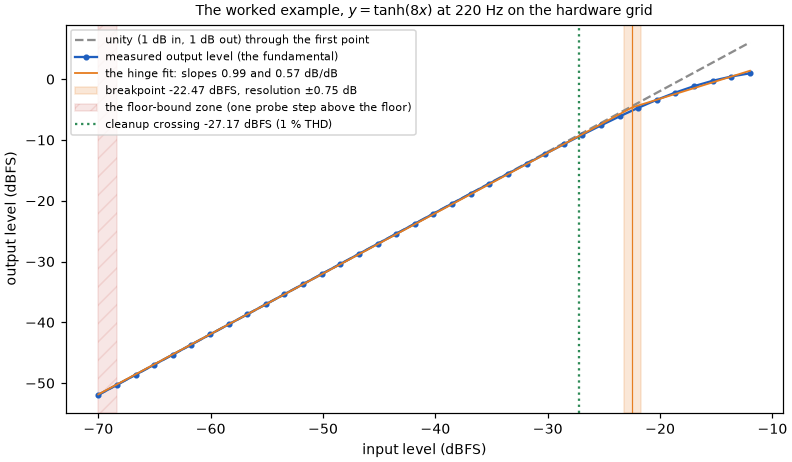
\includegraphics[width=0.95\linewidth]{compression-curve.png}
  \caption{The worked example's curve: $y = \tanh(8x)$ at the default
  note on the hardware grid, output level against input level with the
  unity line through the first point, the hinge fit with its two slopes,
  the breakpoint and its resolution band, the floor-bound zone hatched at
  the quiet end, and the cleanup crossing.}
  \label{fig:compression-curve}
\end{figure}

\begin{figure}[htbp]
  \centering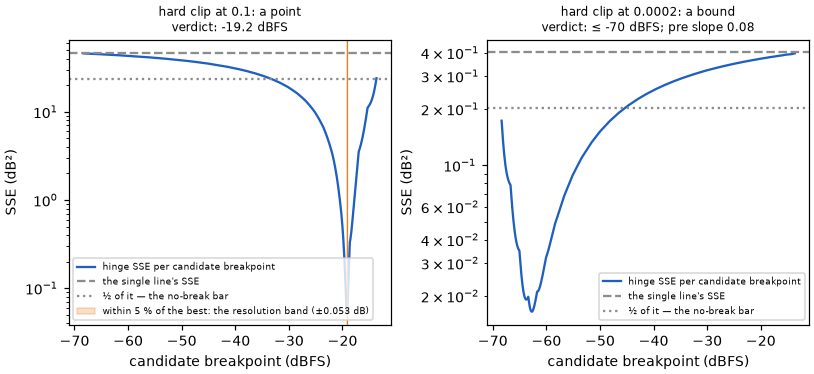
\includegraphics[width=0.95\linewidth]{compression-knee.png}
  \caption{The hinge fit's error over the candidate breakpoints, for a
  hard clipper whose threshold sits inside the window (left: a sharp
  minimum, the five-percent band a width, a point) and for one whose
  threshold sits under the floor (right: the profile falls toward the
  floor with no anchored minimum, and the verdict is a bound at the
  floor by the unity guard).}
  \label{fig:compression-knee}
\end{figure}

\begin{figure}[htbp]
  \centering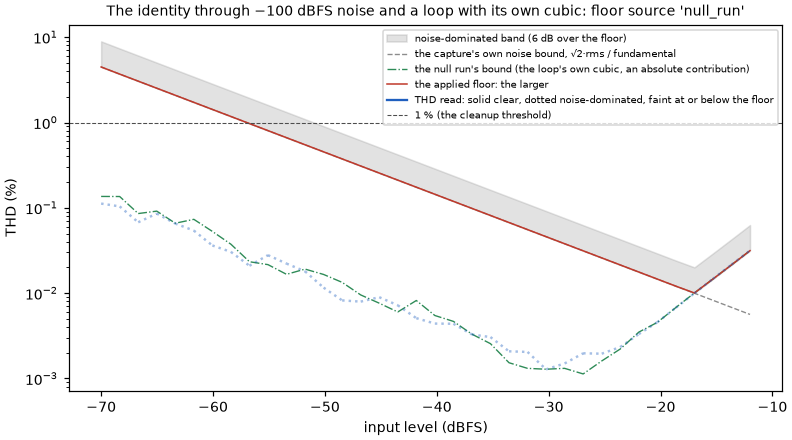
\includegraphics[width=0.95\linewidth]{compression-floor.png}
  \caption{THD against level for the identity through seeded noise and a
  loop with its own cubic: the capture's noise bound of \eqref{eq:noisebound},
  rising toward the quiet end, the null run's bound (the loop's own
  distortion, an absolute contribution, defined inside its probed span
  only), the applied floor as the larger, the noise-dominated band above
  it, and the trace in the chart's three styles --- here at or below the
  floor everywhere, since the identity adds nothing of its own.}
  \label{fig:compression-floor}
\end{figure}

\begin{figure}[htbp]
  \centering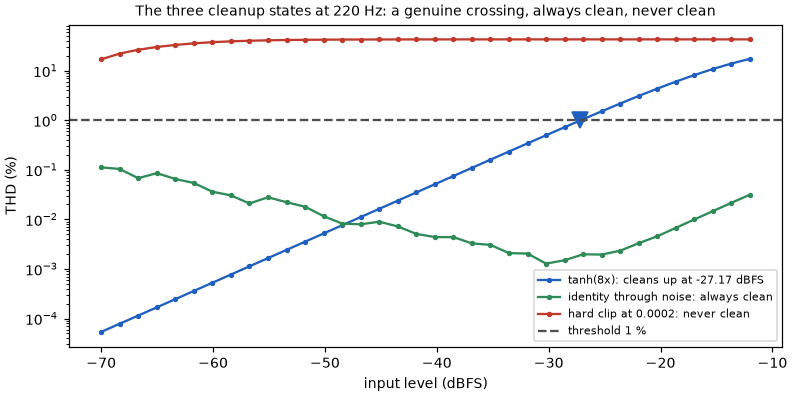
\includegraphics[width=0.85\linewidth]{compression-cleanup.png}
  \caption{The three cleanup states: a genuine crossing interpolated
  between the two steps that straddle the threshold, a curve under the
  threshold at every step (always clean), and a clipper whose threshold
  sits under the grid's floor (never clean).}
  \label{fig:compression-cleanup}
\end{figure}

\begin{figure}[htbp]
  \centering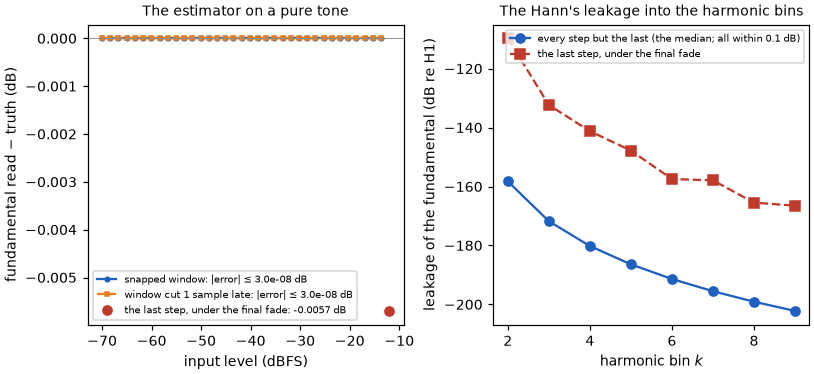
\includegraphics[width=0.95\linewidth]{compression-estimator.png}
  \caption{The estimator on a pure tone (left): the fundamental's read
  against its truth per step on the snapped window and on a window cut
  one sample late --- both at rounding --- and the last step, which
  holds the stimulus's final fade; and the Hann's leakage of the
  fundamental into every harmonic bin (right), by bin distance, on the
  snapped window and under the fade.}
  \label{fig:compression-estimator}
\end{figure}

The app's own rendering of the same measurement kind, from the user
guide's figure pipeline (Figure~\ref{fig:compression-app}).

\begin{figure}[htbp]
  \centering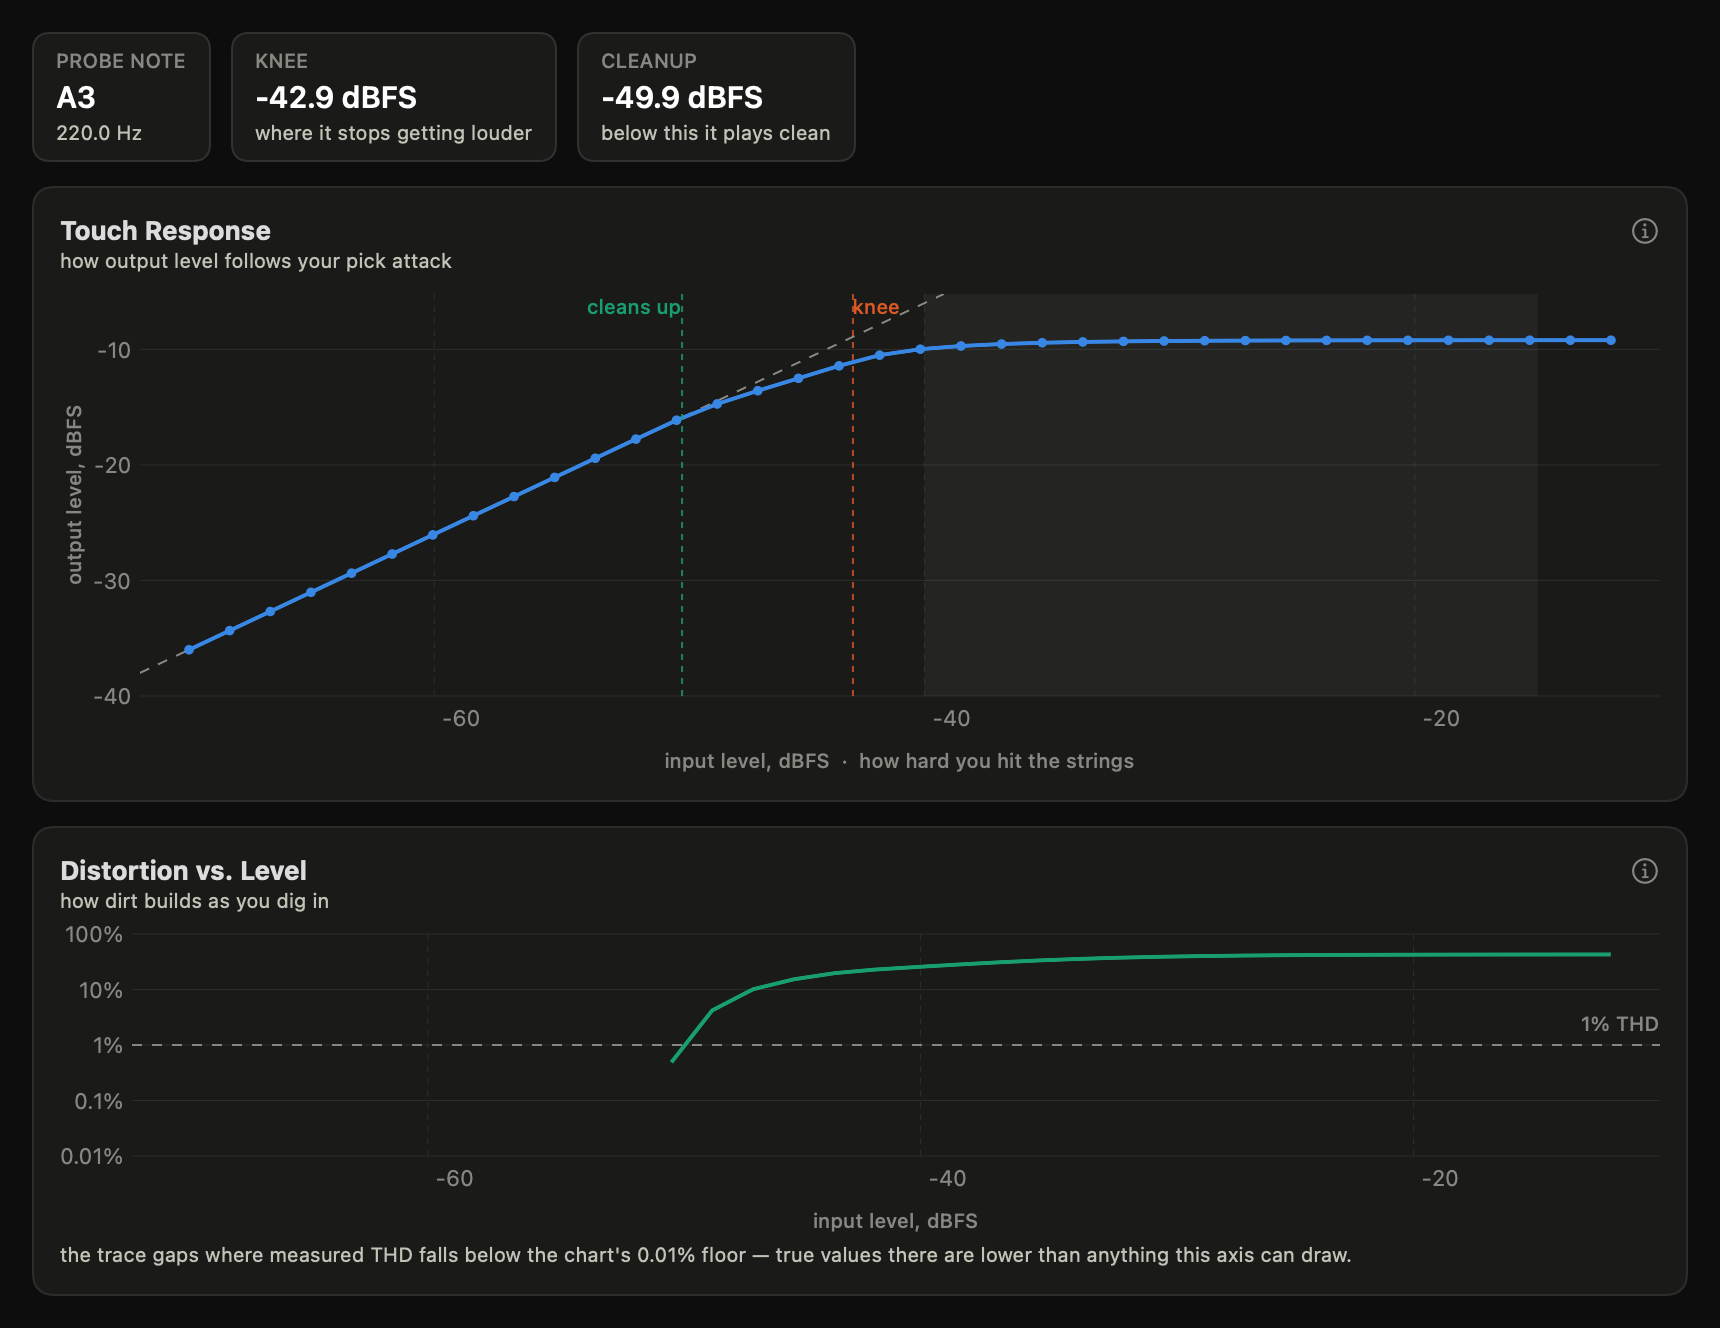
\includegraphics[width=0.85\linewidth]{compression--sim-knee.png}
  \caption{The Compression view as the app draws it, from the guide's
  simulated fixture: the measured output level following the dashed
  unity reference at low levels then flattening, the knee and cleanup
  tiles, and the companion THD trace below with its gap under the
  chart's own floor.}
  \label{fig:compression-app}
\end{figure}

\subsection{Worked example and parity}
\label{sec:compression-example}
The \term{parity} runs \cparityCaseCount\ cases through both
implementations and two device cases again as their \term{phantom} twins
(\cparityTwinCount\ twins). The Python imports chapter one's device family
and noise generator and the transfer chapter's filters, and owns the rest:
this instrument has no sweep. Every case is a known device through a
known LOOP --- a delay, one seeded noise stream referred to the
interface's input, a chain gain applied after both, and optionally the
loop's own cubic, the converter's distortion --- inside the app's
assembly, and beside every step the oracle prints its truth: the
memoryless device's closed-form ladder at that step's drive (chapter
one's quadrature, one pass for all orders, the fundamental's own
compression included, the loop's cubic composed where it is set), scaled
by a pre-filter's magnitude at $f_0$, a post-filter's at $k f_0$ and the
chain gain; the truth THD as \eqref{eq:cthd}'s order rule applied to that
ladder; and the read-time half as the shipped predicates run on a curve
built from the truth points --- the definition applied to the ladder,
never a second derivation. A knee has no analytic truth beyond that: a
hinge fit is a summary of a curve, not a property of the device.

The instrument every truth comparison rests on is the estimator's own
leakage: the pure phantom $[1]$, whose truth is zero at every order above
the first, read on the tone's own geometry. The symmetric Hann leaks a
tone into the other bins by bin distance --- \cparityLeakageOne\ dB re the
tone at one bin, \cparityLeakageTwo\ at two, \cparityLeakageEight\ at
eight --- level-invariant to rounding:
\begin{center}\small\cparityLeakageTable\end{center}
A content order can read up to its truth plus what every OTHER present
order leaks into its bin, $20\log_{10}(1 + \Lambda_k / a_k)$ with
$\Lambda_k$ the sum by distance; that allowance is subtracted before the
bar is applied, and what remains is the method's own error (measured: the
read sits AT the allowance, to two percent). Under the final fade the
one-bin leakage rises to \cparityFadeLeakageOne\ dB, which is why the
last step is excluded from every comparison and why the fade is a stated
limit. \machineFloorNote{} The test asserts:
{\sloppy
\begin{itemize}
  \item Swift against Python: every header quantity and every measured
  column within \cparitySwiftTolerance\ dB (measured maximum
  \cparityWorstSwift\ on this run) on a capture with no filter in it and
  within \cparitySwiftFilteredTolerance\ (measured
  \cparityWorstSwiftFiltered) through a biquad; the two quadratures'
  truth columns within \cparitySwiftTruthTolerance\ (measured
  \cparityWorstSwiftTruth); every discrete reading --- the gate's
  verdict per step, every class, every run, the knee's state and bound,
  its label, the cleanup state, the floor label with and without the
  null run, the presence verdict --- identical; dust (a harmonic whose
  truth sits more than \cparityEmptyDepth\ dB under the fundamental) is
  stated and not compared;
  \item the shipped read against the ladder on every noiseless case,
  every step but the last: the fundamental within \cparityHOne\ dB
  (measured \cparityWorstHOne); the content harmonics after the
  allowance within \cparityTruthSmooth\ for the smooth devices (measured
  residue \cparityWorstResidueSmooth), \cparityTruthKinked\ for the hard
  clipper (\cparityWorstResidueKinked\ --- at the default note and rate no
  alias image of a per-sample device lands on a harmonic bin, since the
  rate is not an integer multiple of the note, so the kinked device reads
  like a smooth one here; its twin \cparityWorstResiduePhantom) and
  \cparityTruthFiltered\ through a filter (\cparityWorstResidueFiltered);
  the THD after the allowance summed over every bin the analyzer sums
  within \cparityTHD\ (\cparityWorstTHDResidue); the last step's
  fundamental LOW by the fade, between \cparityWorstFade\ and
  \cparityLeastFade\ dB (the bar \cparityFade\ --- a compressing device
  flattens the fade);
  \item the knee against the truth curve's knee within \cparityKnee\ dB
  (measured \cparityWorstKnee\ --- every point knee on the hardware grid
  lands on the same candidate, and the two that differ do so by one
  candidate step), and the cleanup crossing within \cparityCleanup\
  (\cparityWorstCleanup);
  \item the stamp against the injected noise within \cparityStamp\ dB
  (measured \cparityStampError\ --- the pre-roll estimate's own scatter);
  the same device and noise through a loop 12 dB louder: the knee's input
  level moved by \cparityGainKneeMove, every class equal, every output
  level moved by 12 dB with a departure of \cparityGainShift\ (bar
  \cparityGain); a capture \cparityLatencyFound\ samples late with the
  analyzer told the pre-roll plus that: every read against the undelayed
  capture within \cparityLatencyMove\ (bar \cparityLatency); a window cut \cparityMiscutSamples\ sample late: the
  fundamental moved by \cparityMiscutMove\ dB (bar \cparityMiscut) ---
  the Hann's taper makes a one-sample mis-cut invisible;
  \item Part B on the oracle's loops: the identity through noise reading
  every point at or below the noise bound (the bathtub), always clean, no
  knee; the null run through a linear loop labelled capture noise (its
  bound sits under this capture's stamp everywhere) and through a loop
  with its own cubic labelled null run, its bound nil outside its span;
  the four verdict legs on their fixtures; the fine window keeping the
  local probe step; the plugin window's ceiling at exactly 0 dBFS; the
  stated floor governing; the device with no fundamental refused
  everywhere; and the one-bin estimator's own separation on a phantom
  with no fundamental, \cparitySeparation\ dB against the borrowed
  \cparitySeparationBar\ dB bar (pinned to stand over it by
  \cparitySeparationOverBar\ dB).
\end{itemize}
\par}
\cparityPartBStatus

The device cases, each with its content-harmonic count, its
Swift-vs-Python figure, its fundamental's error, its worst raw harmonic
error and where, its residue after the allowance, its THD residue and
its fade:

\begin{center}\scriptsize\setlength{\tabcolsep}{3pt}\cparityDeviceTable\end{center}

Every case's read-time verdicts on the Swift side --- the knee the page
would print, the cleanup, the floor label --- with the two
implementations' agreement:

\begin{center}\scriptsize\setlength{\tabcolsep}{3pt}\cparityReadTimeTable\end{center}

The worked example, $y = \tanh(8x)$ noiseless on the hardware grid:
\cparityWorkedContent\ content harmonics compared, the fundamental within
\cparityWorkedHOne\ dB, the worst raw harmonic error \cparityWorkedRaw\ dB
at \cparityWorkedRawAt\ and \cparityWorkedResidue\ dB after the allowance
(at \cparityWorkedResidueAt), a THD residue of \cparityWorkedTHDResidue\
dB, the last step \cparityWorkedFade\ dB under its truth. Its knee is a
point at \cparityWorkedKnee\ dBFS (resolution $\pm$\cparityWorkedKneeResolution\
dB, displayed as ``\cparityWorkedKneeLabel''), slopes
\cparityWorkedPreSlope\ and \cparityWorkedPostSlope\ dB/dB, against the
truth curve's \cparityWorkedTruthKnee\ (a difference of
\cparityWorkedKneeError); its cleanup crossing \cparityWorkedCleanup\ dBFS
against the truth curve's \cparityWorkedTruthCleanup\ (a difference of
\cparityWorkedCleanupError); its summaries read a sharpness of
\cparityWorkedSharpness\ and a top-of-range slope of
\cparityWorkedAsymptote\ dB/dB. The hard clipper at a threshold of
$0.1$: clipping begins at \cparityClipOnset\ dBFS and the fitted
breakpoint sits at \cparityClipKnee\ dBFS, \cparityClipKneeAboveOnset\ dB
above the onset, with a post-knee slope of \cparityClipPostSlope\ and a
resolution of $\pm$\cparityClipResolution\ dB --- a MEASURED relation
between a fit's corner and a clipper's onset, not a claim; with the fine
window over that knee the grid delivers \cparityFineDelivered\ points,
the knee reads \cparityFineKnee\ dBFS at $\pm$\cparityFineKneeResolution\
(the resolution unchanged --- on both grids the five-percent band is
narrower than one candidate step, so the candidate spacing is what the
fit resolves) and moves by \cparityFineKneeMove\ dB. The exact sub-unity
line with a break reads ``\cparityBreakKnee'' with fitted slopes
\cparityBreakPreSlope\ and \cparityBreakPostSlope\ (the unity guard). The
device with no fundamental --- a phantom whose fundamental sits 80 dB
under its second harmonic --- reads absent on \cparityAbsentFraction\ of
its points at a median depth of \cparityAbsentDepth\ dB and no knee, no
cleanup and no floor label. Simulation Mode's assembly on the worked
example (interactive quality: fewer steps, shorter windows, no pre-roll)
reads its knee at \cparitySimulationKnee\ dBFS at
$\pm$\cparitySimulationKneeResolution, \cparitySimulationKneeGap\ dB from
the app assembly's --- what interactive quality costs on this device.

\subsection{Limits and failure modes}
\label{sec:compression-limits}
{\sloppy
\begin{itemize}
  \item \textbf{The last step is measured under the stimulus's own fade.}
  The tone's final fade covers its last ramp length, and the last step's
  measurement window ends where the tone ends, so that window holds the
  fade: the last step's reads sit low (\cparityWorstFade\ to
  \cparityLeastFade\ dB on the parity's devices) and the one-bin leakage
  there rises from \cparityLeakageOne\ to \cparityFadeLeakageOne\ dB. A
  stimulus fact, not a device's --- moving the fade past the window is a
  capture-time change to the corpus's stimulus and is reported, not made.
  \item \textbf{The no-break test has no scale, and the fade can decide
  it.} The first verdict leg compares two residuals as a RATIO; on a
  curve that is one exact sub-unity line the only departure from a line
  is the last step under the fade, the hinge absorbs that one point, the
  ratio reads a break, and the second leg then reads no knee --- where the
  same exact line with no fade reads the bound at the floor. Measured:
  the exact line reads ``\cparityLineMeasuredKnee'' on both
  implementations while its truth curve reads ``\cparityLineTruthKnee''
  with a pre-knee slope of \cparityLineTruthPreSlope; the kernel's own
  fixture for that leg has no fade and passes. The exact line with a break
  is unaffected (the unity guard fires on its fitted pre slope). A
  measured device rarely draws an exact line, and any real curvature
  overwhelms one bent point; the leg is stated as decided by structure the
  test cannot see, and the two mechanisms above are one finding.
  \item \textbf{Skipped steps are silent.} A step whose window runs past
  the capture is dropped with no count, unlike the gate's; a short
  capture yields a shorter curve, and whether the omission deserves a
  stamp is a stored-format question, reported here.
  \item \textbf{The assembly lives in four places.} The record's
  pre-roll, tail, stamp and cut are the app's literals, copied in the
  command-line tool and written differently twice more; the oracle mirrors
  the app's and says so, and a shipped plan is the filed follow-up. Until
  it lands, the mirror is the one place this chapter's pipeline is not the
  shipped code called.
  \item \textbf{A soft onset is not disclosed.} The unity guard tells a
  clean anchor from a missing one; it does not tell a wide soft onset from
  a corner. A drive-max soft-knee overdrive record in the library reads a
  unity bottom decade and a wide soft onset above it, and its point knee
  is honest as far as the fit goes; a transition-width disclosure would be
  a new mechanism, not a tolerance.
  \item \textbf{The borrowed bar.} The presence separation was measured
  for the sweep analyzer; the one-bin estimator separates a fundamental
  from its harmonics by \cparitySeparation\ dB on a snapped window, so
  the bar is conservative here by a wide margin, never optimistic.
  \item \textbf{One note.} The curve is one pitch; a device with a tone
  network ahead of its clipper compresses differently at another, and the
  Gain Map (\S\ref{sec:journey}) is the cross-check across notes.
  \item \textbf{The quiet end is the rig's.} Below the noise bound the
  read is the rig, and the classes say so per point; a low-level upturn in
  THD is the bathtub, not the device, unless it stands clear of the band.
  \item \textbf{Aliasing in a simulated device.} A device applied per
  sample folds its content above Nyquist onto the reads; at the default
  note and rate no image lands on a harmonic bin, and the parity's twins
  are the alias-free control. At another note or rate a kinked device's
  high orders would not be the oracle for that bin.
\end{itemize}
\par}

\clearpage
\section{Gain Map}
\label{sec:journey}
% The residue fragment defines macros the stimulus and predicate sections
% quote before the parameter table prints its table, so it is input here.
% GENERATED by gen_docs.py from generated/manifest.json — do not edit
\newcommand{\journeyResidueTable}{
\begin{tabular}{@{}rrrrrr@{}}
\toprule $j$ & $f_j$ (Hz) & 2 s & 5 s & 10 s & worst \\ \midrule
0 & 20 & -21.63 & -27.74 & -34.13 & -21.63 \\
1 & 26.2 & -46.32 & -70.11 & -86.67 & -46.32 \\
2 & 34.33 & -74.85 & -103.6 & -117 & -74.85 \\
3 & 44.99 & -92.87 & -117.2 & -129.3 & -92.87 \\
4 & 58.94 & -104 & -127.2 & -140.3 & -104 \\
5 & 77.23 & -114.2 & -136.3 & -150.4 & -114.2 \\
6 & 101.2 & -123 & -144.4 & -160 & -123 \\
7 & 132.6 & -130.2 & -152.1 & -169 & -130.2 \\
\bottomrule
\end{tabular}
}
\newcommand{\journeyResidueColumnOneHz}{26.2}
\newcommand{\journeyResidueColumnOneTwo}{-46.32}
\newcommand{\journeyResidueColumnTwoTwo}{-74.85}
\newcommand{\journeyResidueColumnOneFive}{-70.11}
\newcommand{\journeyResidueColumnTwoFive}{-103.6}
\newcommand{\journeyResidueColumnOneTen}{-86.67}
\newcommand{\journeyResidueColumnTwoTen}{-117}
\newcommand{\journeyResidueWorstColumnOne}{-46.32}
\newcommand{\journeyHardwareStep}{5.143}
\newcommand{\journeyPluginStep}{8.571}
\newcommand{\journeyStampMedianOctaves}{0.25}


\subsection{Purpose, and what the measurement cannot tell you}
A \term{gain-map} is the Harmonic Distortion measurement of
\S\ref{sec:hd} repeated at each \term{drive-level} of a \term{level-lattice}
--- one sweep per level, each level analyzed on its own --- and summarized
on one grid: for every level $i$ and every column $j$ of an
\term{export-grid} of fundamentals, the \term{thd} over the audible band and
the level of every stored \term{harmonic-order}, each a \term{map-cell}. It
answers what one sweep cannot: how the harmonic content moves with how hard
the device is driven --- whether it cleans up, where, and whether its
recipe holds across the range. At read time the record states a
\term{peak-tile} (the loudest cell that is a measurement, or a bound), a
\term{cleanup-reading} per column and one tile at the Compression probe's
note, and a \term{fundamental-presence} verdict over the map.

What it cannot tell you, stated once: (a) anything about the device's
output level or gain --- the cells are ratios to each level's own
fundamental, and the drive axis is the signal driving the circuit, never a
knob on it (to map a knob is to measure one map per position); (b) anything
between two levels --- the rows are separate captures seconds apart, and a
circuit that drifts or sags between them shows the drift as row-to-row
wobble; (c) whether a cell near its floor is the device or the rig ---
below the \term{composed-margin} a cell is quoted as a bound; (d) anything
at the two \term{edge-mask} columns, which are the sweep's own fade ramps;
(e) anything a \term{truncated-column} lost above the top of the band; and
(f) anything about what the distortion sounds like.

\subsection{The stimulus}
\label{sec:journey-stimulus}
The lattice is $N$ levels evenly spaced in dB from a floor to a ceiling
inclusive,
\begin{equation}
  \ell_i = \ell_{\min} + (\ell_{\max} - \ell_{\min})\,\frac{i}{N - 1},
  \qquad A_i = 10^{\ell_i/20},\qquad i = 0 \ldots N-1,
  \label{eq:lattice}
\end{equation}
a count of one being the ceiling alone. Two \term{drive-window}s exist. The
hardware window is anchored to gain staging: with the interface's input
staged so that pedal peaks land in the staging target at the loudest
planned drive, the ceiling is the loudest drive that cannot clip the
converter, and the floor sits a fixed travel below it (a step of
\journeyHardwareStep\ dB on the default lattice). The plugin window's ceiling
is digital full scale --- the float render path has no converter to protect
--- and its floor is lower, where high-gain preamp knees were measured to
sit (a step of \journeyPluginStep\ dB). The parameter table gives both.

Each level's stimulus is the synchronized sweep of \S\ref{sec:hd-stimulus}
at that level's amplitude --- the same band, the same requested length, the
same fades --- between a pre-roll of silence (the per-level noise region)
and a tail of silence:
\begin{equation}
  s_i[n] = \big[\underbrace{0,\ldots,0}_{\lfloor t_{\mathrm{pre}} f_s\rfloor},\;
  x_i[0], \ldots, x_i[S-1],\;
  \underbrace{0,\ldots,0}_{\lfloor t_{\mathrm{tail}} f_s\rfloor}\big],
  \label{eq:journeystep}
\end{equation}
with $S$ the sweep's sample count. The sweep length is the measure
sheet's pick from a short list and is \emph{not stored} in the record;
the consequence is a floor derivation that must take the worst case over
the list (\S\ref{sec:journey-floor}). The default length is shorter than
the fingerprint sweep's, so every extraction window is shorter and the
analyzer separates orders less well at the band's low edge
(\S\ref{sec:journey-example} measures it).

\subsection{The pipeline}
\label{sec:journey-pipeline}
Given the $N$ captured outputs $y_i[n]$ and the loop's integer latency
$\ell$ (the calibration's own measured figure on the hardware path; zero
on the plugin path, which measures and removes its latency per capture):
{\sloppy
\begin{enumerate}
\item \textbf{The aligned cut.} From each capture the sweep and its tail
are cut at the pre-roll plus the latency,
$y_i[\lfloor t_{\mathrm{pre}} f_s\rfloor + \ell \;\ldots\; \lfloor t_{\mathrm{pre}} f_s\rfloor + \ell + S + \lfloor t_{\mathrm{tail}} f_s\rfloor)$,
clipped to the capture's end --- one arithmetic for every caller.

\item \textbf{The per-level analysis.} Each aligned capture goes through
the analysis of \S\ref{sec:hd-pipeline} with the level's own sweep and the
journey's configuration: the same harmonic count, a response DFT half the
fingerprint analyzer's length (twice its bin width), the same window cap.
The levels are analyzed in parallel --- the analyses are pure --- and the
entries sort by ascending amplitude. Nothing is compensated: the loop's
gain and response stay in every order.

\item \textbf{The summary grid.} On the export grid
$f_j = f_1 (f_2/f_1)^{j/(n-1)}$, $j = 0 \ldots n-1$ --- $n$ fundamentals
log-spaced from the sweep's start to its end \emph{inclusive}, so the
first and last columns sit at the sweep's edges --- each level's THD over
the audible band $B$ and each stored order's level:
\begin{equation}
  \mathrm{thd}[i][j] = \frac{\sqrt{\sum_{k \ge 2,\; k f_j \in B,\; \mathrm{valid}_i(k, f_j)} |H^{(i)}_k(k f_j)|^2}}{|H^{(i)}_1(f_j)|},
  \qquad
  h[k][i][j] = 20\log_{10}|H^{(i)}_k(k f_j)|,
  \label{eq:journeycells}
\end{equation}
nil where the fundamental reads zero or the harmonic sits at or above
Nyquist; $\mathrm{valid}_i$ is the level's own \term{validity-bound} ---
the sweep's alias-image bound and nothing else, since the journey is
uncompensated and has no calibrated band. Because the cells are
uncompensated, a cell's \term{delivered-fundamental}, $\ell_i + h[1][i][j]$,
is the level the note actually reached at the converter in absolute
dBFS; the floor's drive term reads it.

\item \textbf{The models.} Beside the grid the record carries one
\term{audition-model} per level --- a Hammerstein fit of that level's
analysis, bounded in level by its own amplitude. The Hear-it panels
consume them and nothing measured does; a render between two levels blends
two fits and the quieter one clamps, inventing a bracket-shaped clipping
the device does not have, measured at $-25$ dB on this lattice --- a
property of what the models \emph{render}, stated here and measured in a
later chapter.

\item \textbf{Storage.} The grid, the levels, the orders, the models, the
sample rate and the integration band. The last two are additive fields: a
legacy record without them derives no validity, no fade, no masks and no
analyzer residue, and its cells summed everything below Nyquist.
\end{enumerate}
\par}

\subsection{Read-time predicates on the result}
\label{sec:journey-predicates}
Everything below is computed from the frozen grid when a record is read.

\paragraph{The validity fade and the truncated columns.} The summary's
validity is the grid's own span with the alias-image bound: a harmonic's
cells past $f_j \le f_s/(2k+1)$ are faded on display. A \term{truncated-column}
is one where some order $k \ge 2$ has $k f_j$ inside the stored band and
fails the bound: its THD cells under-read their declared band, and the
column is flagged and excluded from the tiles, never corrected.

\paragraph{The edge masks.} The two columns within a quarter tone of the
grid's edges --- $f_j \le f_0 \rho$ and $f_j \ge f_{n-1}/\rho$, $\rho$ the
guard ratio --- are the sweep's fade-in and fade-out ramps: excited under a
ramp, they describe the measurement and not the device (a jumpered wire
reproduces them). They are derived from the grid alone, faded, excluded
from the tiles and from the presence vote, and never touch the colour
scale.

\paragraph{Fundamental presence.} Per cell, the reference is the loudest
order \emph{stored} for that cell, the fundamental included; the cell is
absent when the fundamental sits at or beyond the analyzer's separation
bound of \S\ref{sec:hd-predicates} below it, present otherwise,
undetermined without a fundamental read; no rig floor enters. The map's
verdict is the majority over every cell outside the two edge columns, and
it outranks both peak states. The vote is a majority for a reason the
worked example shows: a cell whose fundamental bin holds the loop's noise,
or --- beside the low edge --- the second harmonic's own leakage into the
fundamental's window, reads present on a device that has no fundamental
at all.

\paragraph{The floor, composed from three sources.}
\label{sec:journey-floor}
A cell's THD is quoted as a measurement only where it stands clear of
\emph{every} bound the rig and the analyzer put under it; the applicable
floor is the largest, and the largest floor is the smallest margin.

The first source is the \term{floor-stamp}: the embedded calibration's
THD-versus-frequency curve of the loopback, one read per point at
log-spaced fundamentals, measured once at the calibration's own drive. It
is read through the \term{median-read}: each point replaced by the running
median of its neighbours' dB over an odd window before the interpolation
on the $(\log f, \mathrm{dB})$ plane. The window is a fixed count of
points on the stamp's own grid ($\pm\journeyStampMedianOctaves$ octave,
\journeyStampMedianWindowOctaves\ octave in all --- about
\journeyStampMedianWindowColumns\ of the map's
\journeyColumnOctaves-octave columns, i.e.\ about as wide as one
column) --- wide enough that a single-read trough cannot set the floor. The stamp is a ratio re the calibration's delivered
fundamental, while the cells are uncompensated, so the rig's absolute noise
is the calibration's level plus its measured chain gain, and a cell's
floor ratio is that against the cell's delivered fundamental:
\begin{equation}
  F_{\mathrm{rig}}[i][j] = \mathrm{stamp}_{\mathrm{med}}(f_j) + \max\!\big(0,\; (\ell_{\mathrm{cal}} + G) - (\ell_i + h[1][i][j])\big),
  \label{eq:driveterm}
\end{equation}
the \term{drive-term}. Quieter than the calibration the ratio rises by the
difference, because the noise is absolute; louder, it stays at the stamp's
own ratio --- never extrapolated past what the calibration measured,
because the rig's own distortion rises with drive and the stamp measured
their sum at one drive (the bare loop at the loudest level read a few
thousandths of a percent at 6--16 dB ``clear'' of a floor extrapolated
14 dB below anything the calibration saw). The calibration source
contributes only with both a usable stamp and a chain gain; omitting the
gain left every margin one input-knob setting optimistic.

The second source is a plugin record's \term{operative-floor} --- the
larger of its silence render and its A/A residual, an rms re full scale
--- entering as $20\log_{10}(\sqrt2\,\mathrm{rms}) - (\ell_i + h[1][i][j])$,
an absolute bound with no chain-gain term, because the grid is already
absolute. It governs where the render-path calibration is numerically
silent. The larger of the two ratios is the rig-noise floor; nil when
neither source is usable, since a floor known to be missing a term is
worse than none.

The third source is the \term{analyzer-residue}, and it is what a noise
floor cannot see. The plan's own sweep, handed back as its own capture
with the tail's silence --- nothing in the loop --- goes through the
shipped analyzer at the journey's configuration, and its THD is read per
column of the record's grid: the THD of nothing. One column above the
sweep's start the fade-in ramp leaks \emph{coherently} into the
second-harmonic window: on the shipped grid the residue at
\journeyResidueColumnOneHz\ Hz reads \journeyResidueColumnOneFive\ dB on the
default sweep, \journeyResidueColumnOneTwo\ on the short one and
\journeyResidueColumnOneTen\ on the long one, level-invariant --- a ratio
--- and a column up it is \journeyResidueColumnTwoFive\ dB, under every real
stamp. The sweep length is not stored, so the record takes the worst
(loudest) residue per column over the offered lengths,
\journeyResidueWorstColumnOne\ dB at that column; the residue is computed
at read time from the record's own geometry and cached per grid:
\begin{center}\small\journeyResidueTable\end{center}
The composition is per cell,
\begin{equation}
  m[i][j] = \min\!\Big(20\log_{10}\mathrm{thd}[i][j] - F_{\mathrm{rig}}[i][j],\;
  20\log_{10}\mathrm{thd}[i][j] - R[j]\Big),
  \label{eq:composed}
\end{equation}
the \term{composed-margin}; a cell with no rig-noise margin keeps nil, a
column with no residue keeps the rig-noise margin.

\paragraph{The peak tile.} The truncated and edge columns masked, the
cells whose presence reads absent dropped, the map-level verdict first
(absent $\Rightarrow$ no percentage at all, only the median depth). Pass
one: a cell is \emph{clear} when it is unmasked, measured, and its
composed margin reaches the minimum margin --- every unmasked measured
cell when there are no margins. Pass two: a clear cell is a
\term{corroborated-peak} when the cell one column either side, the same
level one column (\journeyColumnOctaves\ octave, about
\journeyColumnSemitones\ semitones) away, is also clear. The shoulder is
asked for in frequency and never in level: a nonlinearity acting at one
drive acts on the neighbouring notes too and THD moves slowly across one
column's \journeyColumnOctaves\ octave, while across one level step it
can move by tens of dB, so a
genuine onset peak at the loudest level may have no clearing level
neighbour --- and a noise pair in adjacent levels of a single-track column
is as likely as any other pair (measured: two of five bare-loop nulls
paired that way). The tile is the loudest corroborated cell as a peak; else
the loudest unmasked cell as a bound, quoted with $\le$; else nothing.
Without floor information --- Simulation Mode, a record with no
calibration --- every unmasked measured cell counts as clear and
corroborated, and the raw maximum is stated as a peak: reported, not
changed.

\paragraph{The cleanup reading.} A column's $(\ell_i, \mathrm{thd}[i][j])$
pairs, ascending, cells without a THD dropped, read as one of three
states: the first point already at or above the threshold is
\emph{never clean} (within this map's range); the first $i$ with
$\mathrm{thd}_i \ge \tau$ gives \emph{cleans up} at
\begin{equation}
  \ell_{i-1} + \frac{\tau - \mathrm{thd}_{i-1}}{\max(\mathrm{thd}_i - \mathrm{thd}_{i-1},\, \epsilon)}\,(\ell_i - \ell_{i-1}),
  \label{eq:crossing}
\end{equation}
else \emph{always clean} --- the endpoint of the measured range is never
dressed up as a crossing. The threshold is a default-argument literal in
the kernel, read for the manifest by bisecting the shipped initializer;
$\epsilon$ is a literal guard. The tile reads the column nearest, in log
frequency, the Compression probe's own note, so the two records' cleanup
figures are about one pitch, and it is gated on the presence verdict. The
summaries' journey fallback, used only when the Compression kind supplied
no cleanup, reads the column nearest the same note in \emph{linear}
frequency with at least three levels, the same interpolation and a fixed
confidence (all literals). The page adds one rule outside the kernel: a
never-clean tile is scoped to the map's own drive range in its subtitle,
and when the pedal's variant-matched Compression record finds a genuine
crossing below the map's floor the subtitle points there.

\subsection{Parameters}
\label{sec:journey-parameters}
Every value below is read from the manifest, which read it from the
shipped code; the residue capture's drive, the summaries' reference note
and confidence and level count, the crossing guard, the calibrator's grid
start, point count and cut, and the chain gain's grid are literals the
manifest carries as rule strings.

% GENERATED by gen_docs.py from generated/manifest.json — do not edit
\begin{longtable}{@{}p{0.5\linewidth}p{0.45\linewidth}@{}}
\toprule Parameter & Value \\ \midrule \endhead
\multicolumn{2}{@{}l}{\textbf{Drive windows}} \\
hardware window (floor / ceiling / levels) & -48 / -12 dBFS / 8 \\
plugin window (floor / ceiling / levels) & -60 / 0 dBFS / 8 \\
hardware lattice step & 5.143 dB \\
\multicolumn{2}{@{}l}{\textbf{Plan}} \\
sweep band $f_1$ -- $f_2$ & 20 Hz -- 10\,000 Hz \\
sweep length (default) / offered & 5 s / 2, 5, 10 s (not stored) \\
actual duration / rate constant $L$ at the default & 4.97169 s / 0.8 s \\
pre-roll / tail silence & 0.3 s / 0.5 s \\
sample rate $f_s$ (the manifest's) & 96\,000 Hz \\
sweep samples / pre-roll / tail at $f_s$ & 477\,282 / 28\,800 / 48\,000 \\
analyzer: harmonic count $K$ / response DFT $M$ / half-width cap & 9 / 32\,768 / 0.2 s \\
export grid columns & 24 (20--10\,000 Hz inclusive) \\
\multicolumn{2}{@{}l}{\textbf{Summary}} \\
integration band & 20 Hz -- 20\,000 Hz \\
edge mask guard ratio (a quarter tone) & 1.0293022 \\
masked columns on the default grid (bottom / top / truncated) & 0 / 23 / none \\
\multicolumn{2}{@{}l}{\textbf{Floor}} \\
stamp median window (the Gain Map) / per-harmonic path & 7 points / 1 (verbatim) \\
calibration analyzed sweeps / level & 1 / -26 dBFS \\
calibration sweep (the app's) & 20 Hz to round(0.45 $f_s$), 10 s, 0.5 s before / 1 s after \\
residue capture drive & -26 dBFS (a literal; the read is a ratio) \\
\multicolumn{2}{@{}l}{\textbf{Peak tile}} \\
minimum margin & 6 dB \\
\multicolumn{2}{@{}l}{\textbf{Cleanup}} \\
threshold (bisected from the shipped initializer) & 0.01 (1 \%) \\
tile column (nearest in log frequency) & 220 Hz \\
summaries' fallback: reference / minimum levels / confidence & 220 Hz (linear nearest) / 3 / 0.7 (literals) \\
crossing interpolation guard & 1e-12 (a literal) \\
\multicolumn{2}{@{}l}{\textbf{Oracle (\texttt{analysisdump journey-synth})}} \\
ladder quadrature points & 262\,144 \\
\bottomrule
\end{longtable}


\subsection{The result}
\begin{figure}[htbp]
  \centering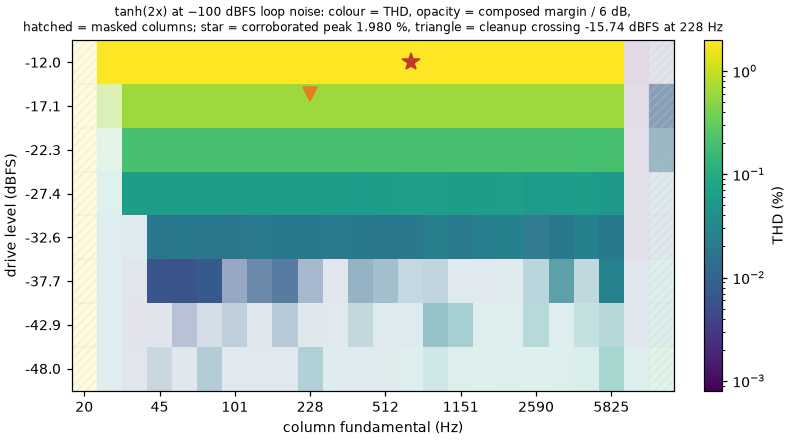
\includegraphics[width=0.95\linewidth]{journey-map.png}
  \caption{The worked example's map: $y = \tanh(2x)$ on the hardware
  lattice through a loop with seeded noise, every cell coloured by its
  THD and drawn at an opacity that follows its composed margin, the two
  edge columns hatched, the corroborated peak starred and the cleanup
  crossing marked at the tile's column.}
  \label{fig:journey-map}
\end{figure}

\begin{figure}[htbp]
  \centering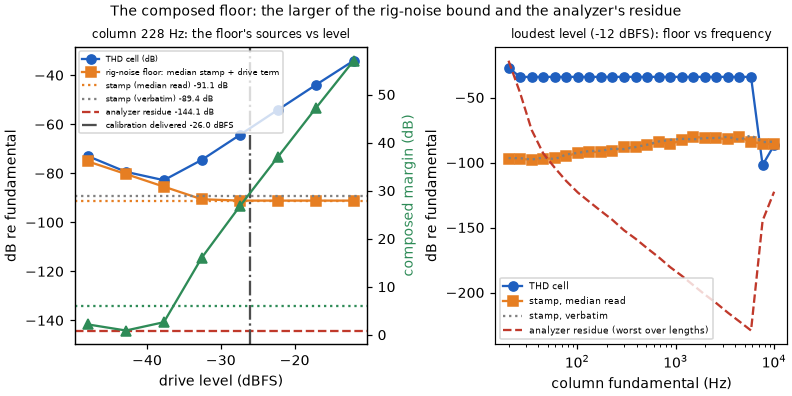
\includegraphics[width=0.95\linewidth]{journey-floor.png}
  \caption{The composed floor at one column against level (left): the
  stamp read verbatim and through the median, the drive term rising below
  the calibration's delivered level and clamped above it, the analyzer's
  residue, and the composed margin against the minimum; and at the loudest
  level against frequency (right).}
  \label{fig:journey-floor}
\end{figure}

\begin{figure}[htbp]
  \centering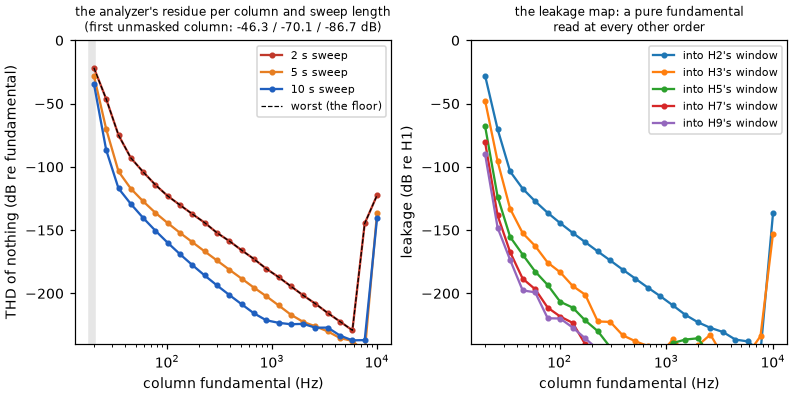
\includegraphics[width=0.95\linewidth]{journey-residue.png}
  \caption{The analyzer's residue per column at the three offered sweep
  lengths (left) --- the fade-in leak at the first unmasked column and the
  worst envelope the record takes --- and the leakage map (right):
  a pure fundamental read at every other order, the parity's own allowance.}
  \label{fig:journey-residue}
\end{figure}

\begin{figure}[htbp]
  \centering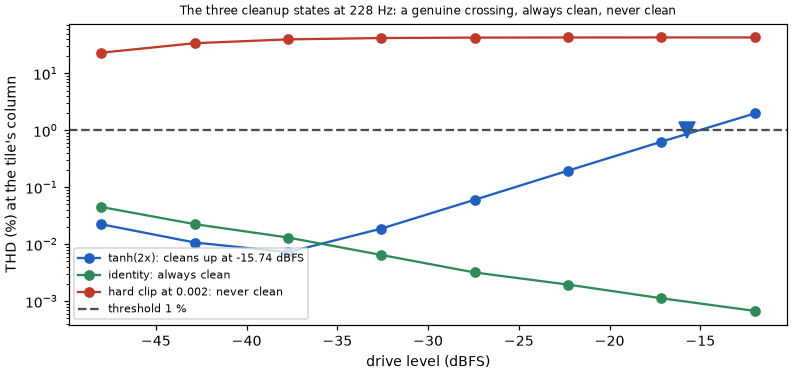
\includegraphics[width=0.85\linewidth]{journey-cleanup.png}
  \caption{THD against level at the tile's column for the three cleanup
  states: a genuine crossing interpolated between two levels, a column
  under the threshold throughout, and a clipper whose threshold sits under
  the lattice's floor.}
  \label{fig:journey-cleanup}
\end{figure}

\begin{figure}[htbp]
  \centering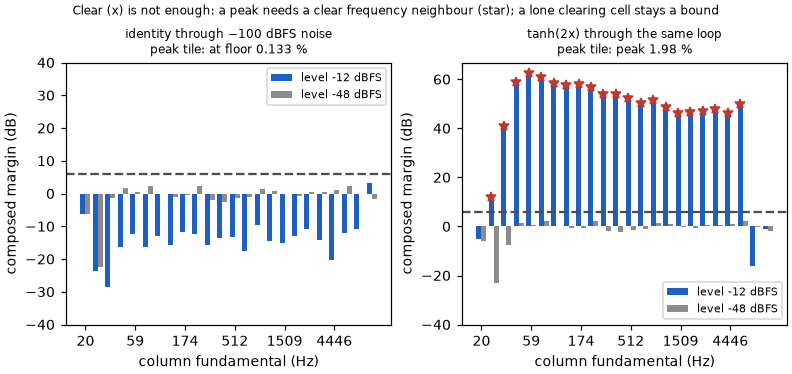
\includegraphics[width=0.95\linewidth]{journey-peak.png}
  \caption{The corroboration rule: composed margins per column at the
  loudest and the quietest level for the identity through noise (left,
  nothing clears and the tile is a bound) and for the soft clipper through
  the same loop (right, every clear cell has a clear neighbour and the tile
  is a peak).}
  \label{fig:journey-peak}
\end{figure}

The app's own rendering of the same measurement kind, from the user
guide's figure pipeline (Figure~\ref{fig:journey-app}).

\begin{figure}[htbp]
  \centering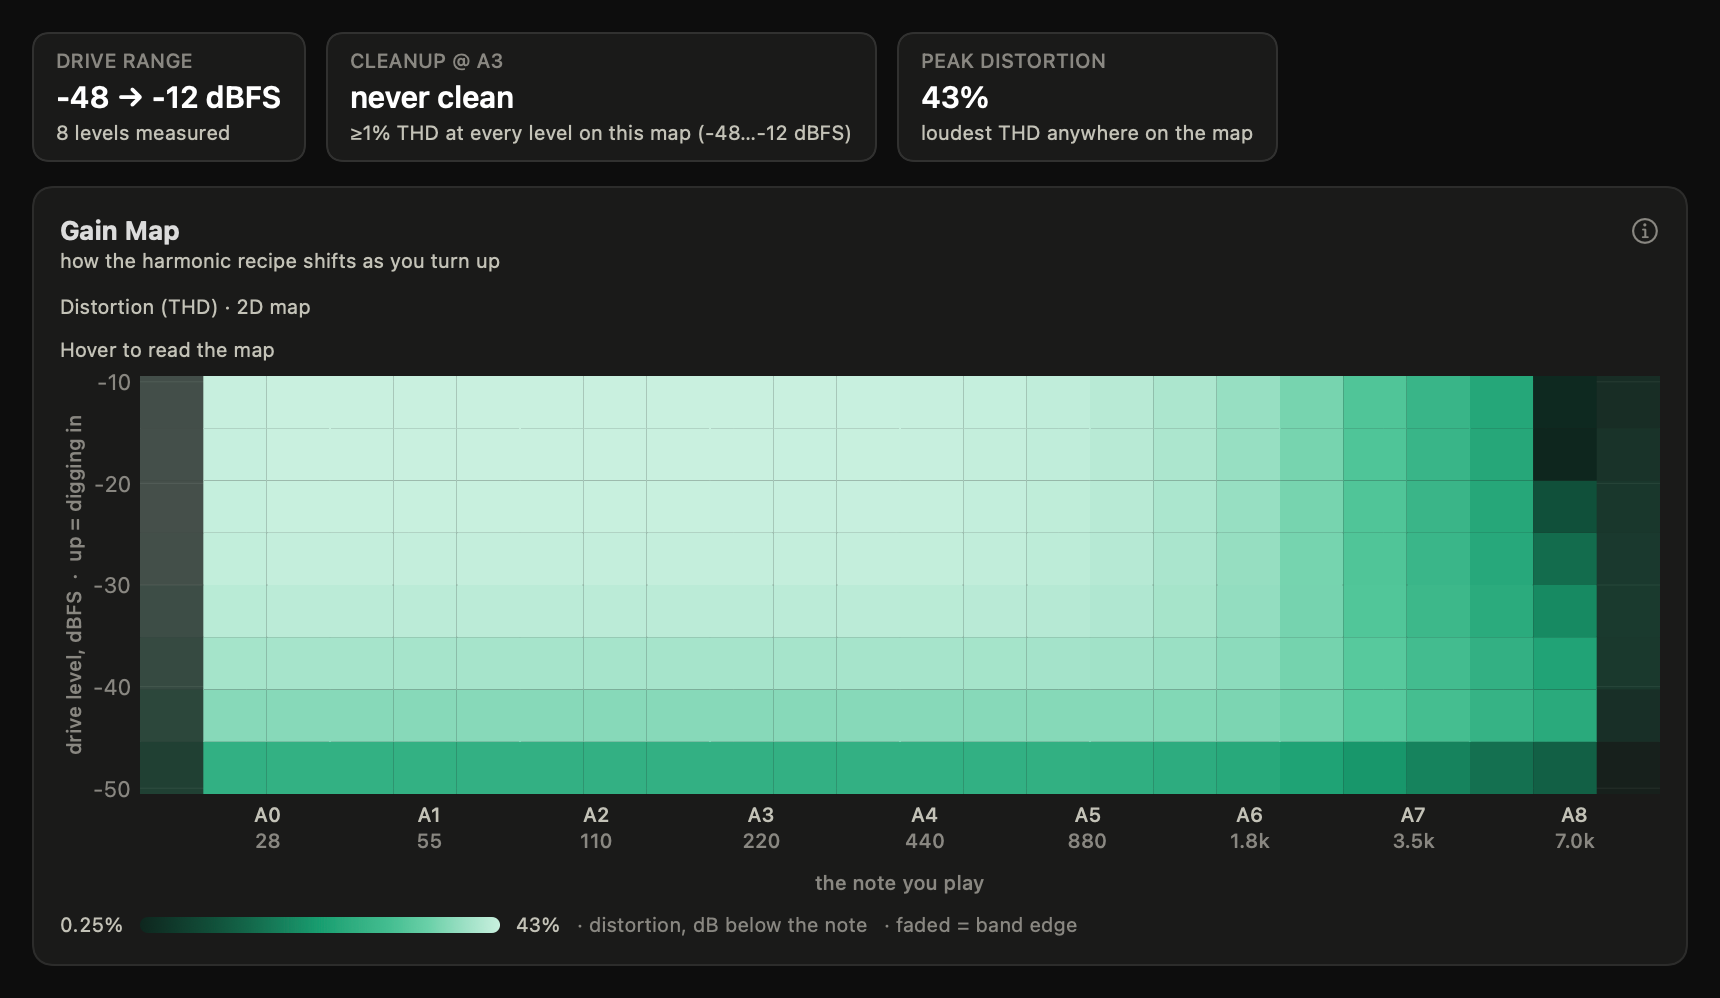
\includegraphics[width=0.85\linewidth]{gain-map--sim-thd-map.png}
  \caption{The Gain Map view as the app draws it, from the guide's
  simulated fixture: the THD map over note and level, the outermost
  columns drawn faded, quiet cells dimmed by their margin.}
  \label{fig:journey-app}
\end{figure}

\subsection{Worked example and parity}
\label{sec:journey-example}
% GENERATED by gen_docs.py from a parity run (Swift vs Python vs the closed-form ladder) — do not edit
\newcommand{\jparitySwiftTolerance}{1e-06}
\newcommand{\jparitySwiftFilteredTolerance}{0.0001}
\newcommand{\jparityEmptyDepth}{140}
\newcommand{\jparityTruthSmooth}{0.05}
\newcommand{\jparityTruthPhantom}{0.05}
\newcommand{\jparityTruthFiltered}{0.3}
\newcommand{\jparityTHDSmooth}{0.001}
\newcommand{\jparityTHDFiltered}{0.2}
\newcommand{\jparityCleanup}{0.3}
\newcommand{\jparityResidueVsLaw}{0.05}
\newcommand{\jparityGainInvariance}{1e-06}
\newcommand{\jparityLatency}{1e-09}
\newcommand{\jparityCorpusPeak}{0.1}
\newcommand{\jparityCorpusBound}{1e-09}
\newcommand{\jparityCaseCount}{15}
\newcommand{\jparityTwinCount}{2}
\newcommand{\jparityWorstSwift}{5.1e-08}
\newcommand{\jparityWorstSwiftFiltered}{1.8e-06}
\newcommand{\jparityLeakageTable}{
\begin{tabular}{@{}rrrrrr@{}}
\toprule $k$ & 26.2 Hz & 34.33 Hz & 44.99 Hz & 58.94 Hz & 173.7 Hz \\ \midrule
2 & -70.13 & -103.6 & -117.2 & -127.2 & -159.5 \\
3 & -95.55 & -133.1 & -152.3 & -162.5 & -201 \\
4 & -112.1 & -145.6 & -163.2 & -176.4 & -217.4 \\
5 & -123.5 & -155.3 & -169.3 & -182.7 & -221.4 \\
6 & -131.9 & -162.7 & -181.1 & -194.2 & -230.5 \\
7 & -138.3 & -167.3 & -188.3 & -196.7 & -240.2 \\
8 & -143.6 & -171.3 & -191.5 & -196.7 & -233.4 \\
9 & -148 & -173.5 & -197.6 & -199.2 & -235.6 \\
\bottomrule
\end{tabular}
}
\newcommand{\jparityLeakageHTwoColumnOne}{-70.13}
\newcommand{\jparityLeakageHThreeColumnOne}{-95.55}
\newcommand{\jparityLeakageHFiveColumnOne}{-123.5}
\newcommand{\jparityLeakageHThreeColumnTwo}{-133.1}
\newcommand{\jparityDeviceTable}{
\begin{tabular}{@{}lrrrrrrrr@{}}
\toprule case & cells & S$-$P (dB) & raw (dB) & at & residue (dB) & 30 dB bar & 40 dB bar & THD residue \\ \midrule
a-tanh & 426 & 5.1e-08 & 0.348 & H5 (4,2) & 0.012 & 0.0978 & 0.0681 & 4e-08 \\
a-tanh-twin & 479 & 1.6e-08 & 0.341 & H5 (4,2) & 0.0051 & 0.0981 & 0.068 & 4e-08 \\
a-poly & 456 & 3.5e-08 & 1.33 & H3 (0,2) & 0.00037 & 0.17 & 0.0534 & 6.4e-05 \\
a-poly-twin & 504 & 1.6e-08 & 1.52 & H3 (0,2) & 0.04 & 0.179 & 0.0545 & 1.7e-05 \\
j-latency & 426 & 5.1e-08 & 0.348 & H5 (4,2) & 0.012 & 0.0978 & 0.0681 & 4e-08 \\
k-tanh-prehp & 421 & 1.2e-06 & 0.215 & H5 (5,2) & 0.15 & 0.215 & 0.155 & 0.09 \\
k-poly-postlp & 456 & 1.8e-06 & 1.34 & H3 (0,2) & 0.00038 & 0.169 & 0.0544 & 7.1e-05 \\
\bottomrule
\end{tabular}
}
\newcommand{\jparityReadTimeTable}{
\begin{tabular}{@{}llrlrrr@{}}
\toprule case & peak tile & value (\%) & cleanup tile & level (dBFS) & absent & S$-$P (dB) \\ \midrule
b-identity-2s & at floor ($\le$) & 0.4834 & always clean & -- & 0 & 1.6e-08 \\
b-identity-5s & at floor ($\le$) & 0.1332 & always clean & -- & 0 & 1.6e-08 \\
b-identity-10s & at floor ($\le$) & 0.1245 & always clean & -- & 0 & 1.6e-08 \\
c-absent & no fundamental & -- & none & -- & 1 & 1.6e-08 \\
d-never-clean & peak & 43.69 & never clean & -- & 0 & 1.6e-08 \\
e-tanh-gain0 & peak & 1.98 & cleans up & -15.74 & 0 & 5.1e-08 \\
e-tanh-gain12 & peak & 1.98 & cleans up & -15.74 & 0 & 5.1e-08 \\
f-operative & peak & 1.98 & cleans up & -15.74 & 0 & 5.1e-08 \\
g-plugin-hardclip & peak & 41.57 & cleans up & -25.05 & 0 & 1.6e-08 \\
\bottomrule
\end{tabular}
}
\newcommand{\jparityWorkedPeak}{1.979}
\newcommand{\jparityWorkedTruthPeak}{1.979}
\newcommand{\jparityWorkedCleanup}{-15.74}
\newcommand{\jparityWorkedTruthCleanup}{-15.74}
\newcommand{\jparityWorkedCleanupColumnHz}{227.6}
\newcommand{\jparityWorkedContent}{426}
\newcommand{\jparityWorkedRaw}{0.348}
\newcommand{\jparityWorkedRawAt}{H5 (4,2)}
\newcommand{\jparityWorkedResidue}{0.012}
\newcommand{\jparityWorkedThirty}{0.0978}
\newcommand{\jparityWorkedForty}{0.0681}
\newcommand{\jparityWorkedTHDResidue}{4e-08}
\newcommand{\jparityWorkedCleanupError}{0.044}
\newcommand{\jparityBoundThirty}{0.27}
\newcommand{\jparityBoundForty}{0.0864}
\newcommand{\jparityWorstThirty}{0.179}
\newcommand{\jparityWorstForty}{0.0681}
\newcommand{\jparityWorstResidueSmooth}{0.012}
\newcommand{\jparityWorstResiduePhantom}{0.04}
\newcommand{\jparityWorstResidueFiltered}{0.15}
\newcommand{\jparityWorstTHDSmooth}{6.4e-05}
\newcommand{\jparityWorstTHDFiltered}{0.09}
\newcommand{\jparityWorstCleanup}{0.197}
\newcommand{\jparityResiduePythonTwo}{-46.32}
\newcommand{\jparityResidueLawTwo}{-46.3}
\newcommand{\jparityResiduePythonFive}{-70.11}
\newcommand{\jparityResidueLawFive}{-70.1}
\newcommand{\jparityResiduePythonTen}{-86.67}
\newcommand{\jparityResidueLawTen}{-86.7}
\newcommand{\jparityIdentityBound}{0.133}
\newcommand{\jparityGainShift}{12}
\newcommand{\jparityGainMarginMove}{$\le$\,1e-10}
\newcommand{\jparityGainStamp}{12}
\newcommand{\jparityLatencyFound}{100}
\newcommand{\jparityLatencyMove}{$\le$\,1e-10}
\newcommand{\jparityOperativeAbsolute}{-76.99}
\newcommand{\jparityOperativePeak}{1.98}
\newcommand{\jparityOperativeStampFloor}{-101}
\newcommand{\jparityAbsentDepth}{80.03}
\newcommand{\jparityAbsentFraction}{0.79}
\newcommand{\jparityPluginPeak}{41.57}
\newcommand{\jparityPluginCleanup}{-25.05}
\newcommand{\jparityNeverCleanPeak}{43.69}
\newcommand{\jparityCorpusTable}{
\begin{tabular}{@{}rlrr@{}}
\toprule record & tile & Python (\%) & kernel (\%) \\ \midrule
59 & at floor ($\le$) & 0.964566 & 0.964566 \\
428 & at floor ($\le$) & 0.778677 & 0.778677 \\
65 & peak & 11.2116 & 11.2116 \\
446 & peak & 6.21905 & 6.21905 \\
404 & at floor ($\le$) & 0.130628 & 0.130628 \\
410 & at floor ($\le$) & 0.106096 & 0.106096 \\
416 & at floor ($\le$) & 0.119273 & 0.119273 \\
422 & at floor ($\le$) & 0.130136 & 0.130136 \\
464 & at floor ($\le$) & 0.105552 & 0.105552 \\
\bottomrule
\end{tabular}
}
\newcommand{\jparityPartBStatus}{Part B's parity is established: on every read-time case — the identity through noise at the three sweep lengths, the device with no fundamental, the never-clean clipper, the loop 12 dB louder, the operative floor on a silent stamp, and the plugin window — the two implementations agree on every margin, every flag, every tile and every verdict, and on the corpus grids the reimplementation reproduces the kernel's own tiles to the digit.}


The \term{parity} runs \jparityCaseCount\ cases through both implementations
and two device cases again as their \term{phantom} twins
(\jparityTwinCount\ twins). The Python imports chapter one's
reimplementation for the sweep, the device, the phantom, the noise and the
analyzer, and adds only what the map adds. Every case is a known device
through a known LOOP: a delay, one seeded noise stream referred to the
interface's input, and a chain gain applied after the device and the
noise, as an input-gain knob is; the calibration is the app's own sweep on
the identity loop through the same gain and noise, analyzed by the shipped
calibrator, whose \emph{measured} latency cuts every level --- the app's
flow. Beside every cell the oracle prints its truth: the memoryless
device's closed-form ladder at that level's drive (chapter one's
quadrature, one pass for all orders), scaled by a pre-filter's magnitude at
$f_j$, a post-filter's at $k f_j$ and the chain gain, and the truth THD as
\eqref{eq:journeycells} applied to that ladder; and the read-time half is
the shipped predicates run on a summary built from the truth cells --- the
definition applied to the ladder, never a second derivation.

The instrument every truth comparison rests on is the \term{leakage-map}
(Figure~\ref{fig:journey-residue}): the pure phantom $[1]$, whose truth is
zero at every order above the first, read on the journey's geometry. Its
higher-order cells are the analyzer's own leakage into each order's window
per column --- \jparityLeakageHTwoColumnOne\ dB into $H_2$'s at the first
unmasked column, \jparityLeakageHThreeColumnOne\ into $H_3$'s,
\jparityLeakageHFiveColumnOne\ into $H_5$'s; a column up,
\jparityLeakageHThreeColumnTwo\ into $H_3$'s:
\begin{center}\small\jparityLeakageTable\end{center}
A cell whose truth stands $c$ dB above the leakage landing in its window
can read up to $20\log_{10}(1 + 10^{-c/20})$ from the truth by the
analyzer alone --- \jparityBoundThirty\ dB at $c = 30$, \jparityBoundForty\
at $40$ --- and that allowance is subtracted before the bar is applied;
what remains is the method's own error. \machineFloorNote{} The test
asserts:
{\sloppy
\begin{itemize}
  \item Swift against Python: every header quantity and every content
  cell in decibels within \jparitySwiftTolerance\ (measured maximum
  \jparityWorstSwift\ on this run) on a capture with no filter in it, and
  within \jparitySwiftFilteredTolerance\ (measured
  \jparityWorstSwiftFiltered) through a biquad; every discrete reading ---
  mask, presence, clear, corroborated, every tile's state, every column's
  cleanup state --- identical; the stamp point for point; the residue per
  column per length wherever it is a reading (a column two hundred
  decibels down is dust on both sides, stated and not compared, as is a
  harmonic cell whose truth sits more than \jparityEmptyDepth\ dB under the
  fundamental);
  \item the shipped read against the ladder on every noiseless case, after
  the allowance: within \jparityTruthSmooth\ for the smooth devices
  (measured residue \jparityWorstResidueSmooth), within
  \jparityTruthPhantom\ for the twins (\jparityWorstResiduePhantom), within
  \jparityTruthFiltered\ through a pre- or post-filter
  (\jparityWorstResidueFiltered\ --- the truth treats each column's
  fundamental as a steady tone through the filter, and a sweep is not
  steady); the raw error tracks the bound: at 30 dB of clearance the worst
  cell reads \jparityWorstThirty\ dB against the bound's
  \jparityBoundThirty, at 40 dB \jparityWorstForty\ against
  \jparityBoundForty;
  \item the THD cells the same way, the allowance built from the residue
  at that column for the case's own sweep length: within
  \jparityTHDSmooth\ (measured \jparityWorstTHDSmooth) and
  \jparityTHDFiltered\ (\jparityWorstTHDFiltered);
  \item the cleanup crossing per unmasked column against the truth curve's
  crossing within \jparityCleanup\ dB (measured \jparityWorstCleanup, at
  the first unmasked column in every case, where the residue's $H_2$ leak
  sits inside the summed THD);
  \item the identity through noise at the three offered lengths: the
  residue at the first unmasked column reads the law's three figures from
  the Python's own analysis (\jparityResiduePythonTwo\ /
  \jparityResiduePythonFive\ / \jparityResiduePythonTen\ against
  \jparityResidueLawTwo\ / \jparityResidueLawFive\ / \jparityResidueLawTen,
  within \jparityResidueVsLaw), every cell's fundamental present, the peak
  tile a bound (\jparityIdentityBound\,\% at the default length), the
  cleanup tile always clean, and no cell in the loudest row quoted clear;
  \item the \#100 term: the same device and noise through a loop 12 dB
  louder moves $H_1$ by \jparityGainShift\ dB, the stamp's chain gain to
  \jparityGainStamp, and no composed margin by more than
  \jparityGainMarginMove\ dB (bar \jparityGainInvariance);
  \item a capture \jparityLatencyFound\ samples late: the calibrator finds
  the latency and every harmonic cell moves by \jparityLatencyMove\ dB
  (bar \jparityLatency);
  \item Part B on the corpus grids: the Python's tiles against the
  kernel's, the peaks within \jparityCorpusPeak\ dB and the bounds to a
  relative \jparityCorpusBound.
\end{itemize}
\par}
\jparityPartBStatus

The device cases, each with its content-cell count, its Swift-vs-Python
figure, its worst raw error and where, its residue after the allowance,
its worst raw error at the two clearance bars, and its THD residue:

\begin{center}\scriptsize\setlength{\tabcolsep}{3pt}\jparityDeviceTable\end{center}

The read-time cases on the Swift side --- the tiles the page would print
--- with the two implementations' agreement:

\begin{center}\scriptsize\setlength{\tabcolsep}{3pt}\jparityReadTimeTable\end{center}

The worked example, $y = \tanh(2x)$ noiseless on the hardware lattice:
\jparityWorkedContent\ content cells compared, the worst raw error
\jparityWorkedRaw\ dB at \jparityWorkedRawAt\ and \jparityWorkedResidue\ dB
after the allowance, \jparityWorkedThirty\ dB at the 30 dB bar and
\jparityWorkedForty\ at 40, a THD residue of \jparityWorkedTHDResidue\ dB;
its peak tile reads \jparityWorkedPeak\,\% against the truth grid's
\jparityWorkedTruthPeak\,\%, and its cleanup tile \jparityWorkedCleanup\
dBFS at \jparityWorkedCleanupColumnHz\ Hz against the truth curve's
\jparityWorkedTruthCleanup\ (a difference of \jparityWorkedCleanupError\
dB). The device with no fundamental --- a phantom whose fundamental sits
80 dB under its second harmonic --- reads a majority verdict of absent
(\jparityAbsentFraction\ of the cells) at a median depth of
\jparityAbsentDepth\ dB and a tile with no percentage; the cells beside the
low edge read present, because the fundamental's window there holds the
second harmonic's own leakage. The operative-floor case: the render-path
stamp reads \jparityOperativeStampFloor\ dB at its loudest point, the
stated floor enters at \jparityOperativeAbsolute\ dBFS, and the peak reads
\jparityOperativePeak\,\%. The plugin window with the hard clipper: a peak
of \jparityPluginPeak\,\% and a crossing at \jparityPluginCleanup\ dBFS.
The never-clean clipper: \jparityNeverCleanPeak\,\% at every level of its
tile column.

Part B on the corpus --- the kernel test's own transcribed grids and
stamps, the read-time half's one stored-input exception (a stored record
holds results, not a capture, but for the read-time half the stored grid
\emph{is} the input, and these grids are the store's own figures pinned to
the digit by the kernel's test):

\begin{center}\small\jparityCorpusTable\end{center}

\subsection{Limits and failure modes}
\label{sec:journey-limits}
{\sloppy
\begin{itemize}
  \item \textbf{The sweep length is not stored, and the floor pays for
  it.} The residue is taken as the worst over the offered lengths, so a
  record captured at the default length carries the short sweep's residue
  at the first unmasked column, \journeyResidueColumnOneTwo\ dB against its
  own \journeyResidueColumnOneFive: that column's margin is about
  $24$ dB pessimistic --- a bound in the honest direction, and a stored
  length would sharpen it (a stored-format decision, not a read-time one).
  \item \textbf{The fundamental grid is a level, not a normalizer.} The
  cells are uncompensated, so $h[1][i][j]$ is the fundamental as the
  device delivered it through the loop, gain and all. On a device with a
  series resistance ahead of its clipper it is also a load gauge: the same
  reference position measured on two interfaces with different input
  impedances delivers a different fundamental, and every ratio to it is
  taken against that delivered level. The map does not separate the
  device's gain from the loop's, and it does not claim to.
  \item \textbf{The analyzer's separation is geometry-dependent, and the
  journey's geometry is the coarser one.} The default sweep is half the
  fingerprint sweep's length and the response DFT half its length, so the
  leakage of the loudest order into each window at the low edge is worse
  than chapter one's measured bound; the leakage map states it per column
  and order, and a cell whose content sits inside it is the analyzer's,
  not the device's --- which is what the residue and the margins say in a
  real capture, and why a device with no fundamental reads present beside
  the low edge.
  \item \textbf{Aliasing in a simulated device.} A device applied per
  sample folds its content above Nyquist onto the reads; the smooth
  devices' residues above are inside the allowance, the phantom twins are
  the alias-free control, and a kinked device (a hard clipper at playing
  levels) would not be the oracle for a cell near the top of a band.
  \item \textbf{A raw maximum is a peak where no floor exists.} Without a
  calibration or an operative floor every unmasked cell counts as clear
  and corroborated, and the tile states the map's loudest cell as a peak
  --- Simulation Mode and every record with no calibration are in that
  state; reported, not changed.
  \item \textbf{The per-harmonic path reads the stamp verbatim.} The
  \S\ref{sec:hd} distance and the fundamental-presence margin read the
  calibration stamp point by point; the single-read exposure the median
  read removes from this map exists there and is reported, not changed ---
  moving every distance figure in the library is its own measured change.
  \item \textbf{The audition models invent.} The per-level fits are
  consumed by the listening panels only, and a render between two levels
  blends a clamped quieter fit into the louder one; nothing measured reads
  a fit, and the invention's size is a later chapter's measurement.
  \item \textbf{The rows are separate captures.} Each level is its own
  sweep seconds apart; a circuit whose operating point moves between them
  shows it as row-to-row wobble, which the map draws and does not name.
\end{itemize}
\par}

\clearpage
\section{Chord IMD}
\label{sec:imd}
% The lattice fragment defines macros the predicates section quotes
% before the parameter table prints its tables, so it is input here.
% GENERATED by gen_docs.py from generated/manifest.json — do not edit
\newcommand{\imdSnapTable}{
\begin{tabular}{@{}lrrlrrrrr@{}}
\toprule probe & $f_s$ (Hz) & $N$ & tier & $k_1$ : $k_2$ & $g$ & $a$ : $b$ & cents & candidates \\ \midrule
fifth 44100 Hz & 44\,100 & $2^{20}$ & standard resolvable & 2\,616 : 3\,912 & 24 & 109 : 163 & 0.334 / -3.01 & 121 / 3\,061 \\
fifth 48000 Hz & 48\,000 & $2^{20}$ & standard resolvable & 2\,398 : 3\,586 & 22 & 109 : 163 & -3.6 / -6.94 & 109 / 2\,523 \\
fifth 88200 Hz & 88\,200 & $2^{21}$ & standard resolvable & 2\,616 : 3\,912 & 24 & 109 : 163 & 0.334 / -3.01 & 121 / 3\,061 \\
fifth 96000 Hz & 96\,000 & $2^{21}$ & standard resolvable & 2\,398 : 3\,586 & 22 & 109 : 163 & -3.6 / -6.94 & 109 / 2\,523 \\
fifth corpus 96000 Hz / 2\textasciicircum{}17 & 96\,000 & $2^{17}$ & degraded & 150 : 226 & 2 & 75 : 113 & -2.15 / 7.48 & 0 / 8 \\
fifth Simulation Mode interactive & 48\,000 & $2^{15}$ & degraded & 75 : 113 & 1 & 75 : 113 & -2.15 / 7.48 & 0 / 2 \\
major third A2 + C\#3 96000 Hz & 96\,000 & $2^{21}$ & standard resolvable & 2\,400 : 3\,024 & 48 & 50 : 63 & -2.15 / -2.04 & 99 / 2\,127 \\
\bottomrule
\end{tabular}
}
\newcommand{\imdWindowTable}{
\begin{tabular}{@{}lrrrrrrr@{}}
\toprule grid & $f_s$ (Hz) & $N$ & bin (Hz) & stimulus (s) & start & steady end & overrun \\ \midrule
standard 44100 Hz & 44\,100 & $2^{20}$ & 0.042057 & 24.2772 & 11\,025 & 1\,068\,421 & -8\,820 \\
standard 48000 Hz & 48\,000 & $2^{20}$ & 0.045776 & 22.3453 & 12\,000 & 1\,070\,176 & -9\,600 \\
standard 88200 Hz & 88\,200 & $2^{21}$ & 0.042057 & 24.2772 & 22\,050 & 2\,136\,842 & -17\,640 \\
standard 96000 Hz & 96\,000 & $2^{21}$ & 0.045776 & 22.3453 & 24\,000 & 2\,140\,352 & -19\,200 \\
corpus (pre-\#254 B2a) 96000 Hz / 2\textasciicircum{}17 & 96\,000 & $2^{17}$ & 0.73242 & 1.86533 & 24\,000 & 174\,272 & -19\,200 \\
Simulation Mode interactive 48000 Hz / 2\textasciicircum{}15 & 48\,000 & $2^{15}$ & 1.4648 & 1.18267 & 12\,000 & 54\,368 & -9\,600 \\
\bottomrule
\end{tabular}
}
\newcommand{\imdRoleTable}{
\begin{tabular}{@{}rrlrrl@{}}
\toprule $k$ & Hz & pitch & cents & class & role \\ \midrule
1 & 55 & A1 & 0 & 0 & Growl (sub-octave) \\
2 & 110 & A2 & 0 & 0 & Thickening \\
3 & 165 & E3 & 1.96 & 7 & Thickening \\
4 & 220 & A3 & 0 & 0 & Thickening \\
5 & 275 & C♯4 & -13.7 & 4 & Added colour \\
6 & 330 & E4 & 1.96 & 7 & Thickening \\
7 & 385 & G4 & -31.2 & 10 & Sourness (clash) \\
8 & 440 & A4 & 0 & 0 & Thickening \\
9 & 495 & B4 & 3.91 & 2 & Added colour \\
10 & 550 & C♯5 & -13.7 & 4 & Added colour \\
11 & 605 & D♯5 & -48.7 & 6 & Sourness (clash) \\
12 & 660 & E5 & 1.96 & 7 & Thickening \\
13 & 715 & F5 & 40.5 & 8 & Sourness (clash) \\
\bottomrule
\end{tabular}
}
\newcommand{\imdRoleGridHz}{55}
\newcommand{\imdRoleRatio}{2 : 3}
\newcommand{\imdThirdRatio}{4 : 5}
\newcommand{\imdThirdGridHz}{27.5}


\subsection{Purpose, and what the measurement cannot tell you}
A \term{two-tone} plays two sines at a musical interval through the device
at once. A nonlinearity does not treat them separately: it multiplies them,
and the output carries every \term{intermodulation-product}
$m f_1 + n f_2$ for integer $m, n$, whose \term{product-order} $|m| + |n|$
is the lowest polynomial power that can produce it. The result is the level
of every product up to the enumeration ceiling $K$ (the parameter table
gives it, and the count of recipes it admits), each read at one bin of one
long spectrum and quoted in \term{dbc} against the louder played tone; the
two tone amplitudes as the device delivered them; three capture-time
percentage sums (two borrowed from laboratory two-tone standards and one
total, kept for the record as the frozen tile definitions of earlier
builds); and the raw spectrum beside each played tone, stored for the
\term{coherence-check}. At read time every product gets one
\term{product-reading}, the capture states its own \term{capture-floor},
the products are sorted by \term{harmonic-role} on the grid of the
requested interval, and the drive level is stated from the stored
stimulus.

What it cannot tell you, stated once: (a) anything about other drive
levels --- one capture is one operating point, and the products of a
clipper scale with drive faster than anything else about it; (b) whether
a resolved product is the device's or the rig's --- an interface's
converters intermodulate too, and only a control capture with nothing in
the loop separates the two, which the floor cannot do and does not claim
to; (c) which stage moved the notes when the coherence check fails --- a
verdict without an attribution, by design (\S\ref{sec:imd-coherence});
(d) anything below the capture's own floor, and, for the three percentage
sums, anything at all about a floor: they are capture-time sums over the
products the gate passed and carry no bound (\S\ref{sec:imd-limits});
(e) anything about products above order $K$ --- the enumeration is a
small-signal census, and a hard clipper at playing levels has energy at
orders it does not walk; and (f) anything about what the
distortion sounds like.

\subsection{The stimulus}
\label{sec:imd-stimulus}
In this chapter $f_1 < f_2$ are the two played tones (not the sweep band
edges of \S\ref{sec:hd}), $N$ is the \term{analysis-window} length in
samples, $\Delta f = f_s/N$ the bin width, $k_1, k_2$ the bins the two
tones sit on, $K$ the enumeration ceiling, and $(m, n)$ a product's recipe.
The stimulus is two equal sines at a linear combined peak $A$:
\begin{equation}
  x[n] = \tfrac{A}{2}\sin\!\big(2\pi f_1 n/f_s\big) + \tfrac{A}{2}\sin\!\big(2\pi f_2 n/f_s\big),
  \qquad n = 0 \ldots \lfloor T f_s + \tfrac12\rfloor - 1,
  \label{eq:twotone}
\end{equation}
scaled over its first and last $\lfloor t_{\mathrm{fade}} f_s\rfloor$
samples by the raised cosine $\tfrac12(1 - \cos(\pi i/N_{\mathrm{fade}}))$.
The standard peak is the fingerprint sweep's drive, so the products and
the other measurement kinds describe one operating point; the worked
example below uses the loudest drive the hardware sheet offers, where the
reference clippers clip. The notes are named in twelve-tone equal
temperament with A4 $= 440$ Hz (the parameter table gives the default
pair), and the measure sheet offers one probe: the interval. Two
laboratory probes --- an SMPTE-style pair at a fixed ratio and a CCIF
twin-tone --- existed in the code and were retired before 1.0, because a
standard is never moved onto the lattice described next and neither could
be given one; the two percentage keys that carry their names are sums
over recipe sets and are unrelated to the retired probes.

\paragraph{Coherent sampling, the premise --- stated once.} Both tones are
moved onto exact bin centres of the $N$-point window before anything
plays, so each completes a whole number of cycles inside the segment the
analyzer reads, and the segment is windowed \emph{rectangularly}: a tone
that fits the window exactly leaks into no other bin, so there is nothing
to taper and no taper is used, and the floor beneath a record is noise,
not a window's skirt. \term{coherent-sampling} is inherited by every
product: with the tones on bins $k_1, k_2$ the product $(m, n)$ lands on
bin $m k_1 + n k_2$ exactly, because bin numbers add as frequencies do.
That set of bins is the \term{analysis-lattice}. Every step below is a
consequence of this one premise, and the price of it is the coherence
check: a rectangular window's sidelobes fall as $1/(\pi d)$ at $d$ bins
--- excellent, with no margin --- so a tone that drifts during the
capture spills its own skirt across the lattice.

\paragraph{Two numbers describe the lattice.} Write $k_1 = g a$,
$k_2 = g b$ with $\gcd(a, b) = 1$: the \term{reduced-ratio} $a : b$ and
the \term{lattice-spacing} $g = \gcd(k_1, k_2)$. They answer two
different questions. Two recipes share a bin when
$(m - m')\,a = -(n - n')\,b$, which with $a, b$ coprime forces
$m - m' = -jb$, $n - n' = ja$ for some integer $j \ne 0$, so
$|m - m'| + |n - n'| = |j|(a + b) \le 2K$; hence
\begin{equation}
  a + b \;\ge\; 2K + 1
  \label{eq:reducedsum}
\end{equation}
admits no collision up to order $K$ (the bound is tight: at $K = 7$ the
ratio $1 : 13$ collides and every ratio at $15$ is clean). And the integer
combinations of $k_1$ and $k_2$ are exactly the multiples of $g$ (Bézout),
so two distinct lattice points differ by at least $g$ bins, and some pair
by exactly $g$: no product can sit nearer than $g$ bins to another product
or to either tone, at any order. A lattice can pass \eqref{eq:reducedsum}
and still be crowded --- the probe every record before the current
length was captured on shared no bins at a spacing of two --- which is
why the snap buys spacing and not only collision-freedom.

\paragraph{The lattice snap.} The \term{lattice-snap} is decided in two
steps, so that the interval a record asks is one interval at every rate
and length. First the ratio is chosen \emph{once}, against every standard
grid at the same time (the four supported rates, each at the length it
is meant to analyze at): over $a = 1 \ldots \lfloor f_1 \rho / (\beta\,
\Delta f_{\max})\rfloor$ with $\rho = 2^{c/1200}$ the cents budget $c$ as
a ratio and $\beta$ the resolvable-spacing bar, and for each $a$ over
$b = \max(a + 1, \lceil a r/\rho^2\rceil) \ldots \lfloor a r \rho^2\rfloor$
with $r = f_2/f_1$, a coprime pair satisfying \eqref{eq:reducedsum} is a
candidate; it survives when on \emph{every} standard grid some multiple
$g \ge \beta$ places both $g a\,\Delta f$ and $g b\,\Delta f$ inside
$\pm c$ of the requested tones (the placement on one grid is the in-budget
$g$ with the smallest worst-case pitch error, ties to the smaller $g$).
The survivors are ranked by the interval nearest the requested one, then
the wider minimum spacing, then the smaller $a + b$, then $(a, b)$. The
default fifth lands on the ratio the parameter table quotes, a few cents
flat of equal temperament and the same at every rate; the snap table in
\S\ref{sec:imd-parameters} is that search run by the shipped code on every
grid. Second, on the grid at hand, the standard ratio is scaled: the
in-budget multiple with the smallest pitch error at \emph{any} spacing ---
keeping the interval outranks clearing the bar, so a grid too coarse to
resolve it (Simulation Mode's interactive preview) still asks the same
musical question, in a degraded regime the read-time predicates carry.
Only when no multiple of the ratio fits the budget does the older search
run: every bin pair $(k_1, k_2)$ inside the budget (the half-widths
searched are derived from the budget and the bin width, never fixed),
ranked by spacing, then worst-case cents, then index; the best pair
clearing both \eqref{eq:reducedsum} and $g \ge \beta$ is emitted as
\emph{resolvable}, else the best clearing \eqref{eq:reducedsum} alone as
\emph{degraded} --- which at the old length is the corpus probe, field
for field --- else the plan \emph{refuses} before anything plays, quoting
the widest lattice the budget reached with its reduced ratio, spacing and
sum against the bound. The plain snap is never returned as a fallback: an
exactly degenerate probe drops colliding products through the
enumeration's tie-break and reports a suspiciously clean record.

\paragraph{The window is a duration, and the stimulus is sized to hold
it.} The standard analysis length is stated at the standard rate as a
sample count, but what it fixes is a \emph{duration}: each rate takes the
power of two nearest $N_{\mathrm{std}}\,f_s/f_{s,\mathrm{std}}$, capped
at the plan's ceiling, so the four rates form two grid classes with the
same bin width in pairs. The stimulus duration is then derived from the
length it must hold,
\begin{equation}
  T = t_{\mathrm{fade}} + t_{\mathrm{settle}} + N/f_s + t_{\mathrm{fade}} + t_{\mathrm{settle}},
  \label{eq:imdduration}
\end{equation}
never set by hand: a hand-set duration is how an earlier fixed window
came to overrun the fade-out at two of the four rates
(Figure~\ref{fig:imd-window}). The analysis length a stored stimulus is
read at is derived by the same rule in reverse --- from the ceiling, halve
while the window would overrun the steady state --- so the stimulus is
snapped to exactly the length it is analyzed at, and a shorter snap grid
is a subset of a longer window's bins, never the reverse.

\begin{figure}[htbp]
  \centering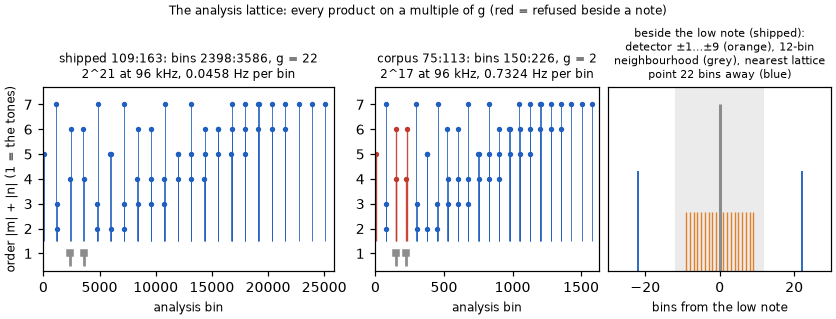
\includegraphics[width=0.95\linewidth]{imd-lattice.png}
  \caption{The analysis lattice: every enumerated recipe as a stem at its
  bin and order on the shipped fifth (left) and on the corpus probe every
  earlier record was captured on (middle), the two tones as squares at
  order one. On the corpus probe the four even-order recipes two bins
  from the played notes and the one two bins from DC draw red: refused on
  position (\S\ref{sec:imd-reading}). Right: the bins beside the low note
  on the shipped lattice --- the detector's offsets, the played-tone
  neighbourhood, and the nearest lattice point a spacing away.}
  \label{fig:imd-lattice}
\end{figure}

\begin{figure}[htbp]
  \centering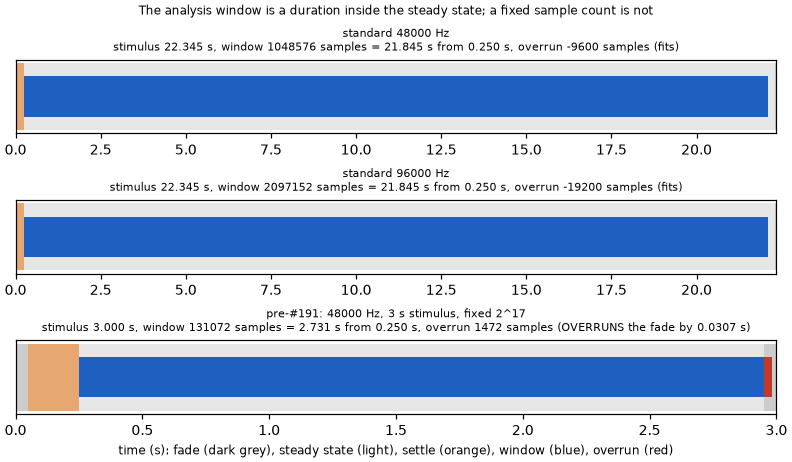
\includegraphics[width=0.95\linewidth]{imd-window.png}
  \caption{The analysis window inside the stimulus at the two 96 kHz-class
  rates, and the historical fixed-length window on a hand-set stimulus at
  48 kHz, which overran the fade-out: periodicity broke and the window's
  own skirt flooded the low bins. The fade-contaminated separation bound
  in the parameter table exists for captures made that way.}
  \label{fig:imd-window}
\end{figure}

\subsection{The pipeline}
\label{sec:imd-pipeline}
Given the captured output $y[n]$ and the integer loop latency $\ell$ (the
app measures and removes it per capture; the oracle renders at zero
latency and, when asked, analyzes with a deliberate offset):

{\sloppy
\begin{enumerate}
\item \textbf{The window.} The segment starts at
$s = \ell + \lfloor t_{\mathrm{fade}} f_s\rfloor + \lfloor t_{\mathrm{settle}} f_s\rfloor$
and runs for exactly $N$ samples, rectangularly windowed and zero-padded
if the capture ends first; the steady state ends at
$e = \ell + \lfloor T f_s + \tfrac12\rfloor - \lfloor t_{\mathrm{fade}} f_s\rfloor$,
and the \emph{overrun} $s + N - e$ is positive when the segment would
swallow the fade-out. Latency shifts $s$ and $e$ alike, so a window that
fits at zero latency fits at any, and because the tones are bin-centred a
shift is a phase: no magnitude moves (\S\ref{sec:imd-example} measures
it). The analyzer never shortens a window it is handed --- the tones are
centred on the length the stimulus was snapped to, and a shorter
rectangular window would leak far worse than the fade it avoided.

\item \textbf{The spectrum.} With $c$ the number of captured samples inside
the segment,
\begin{equation}
  M[b] = \frac{2}{\min(N, c)}\,\Big|\mathrm{DFT}_N\{y[s + i]\}[b]\Big|,\qquad b = 0 \ldots N/2,
  \label{eq:imdmag}
\end{equation}
so a bin-centred sine of amplitude $a$ reads $a$.

\item \textbf{The enumeration and the lattice.} With $\mathrm{bin}(f) =
\mathrm{round}(f/\Delta f)$, the set $S = \{\mathrm{bin}(f_1), \mathrm{bin}(f_2), 0\}$
is seeded, and the walk runs order $= 2 \ldots K$, $m = -\mathrm{order}
\ldots \mathrm{order}$, $n = +(\mathrm{order} - |m|)$ then
$-(\mathrm{order} - |m|)$: a recipe with $\Delta f < m f_1 + n f_2 <
0.95\,f_s/2$ (both edges literals) whose bin is not yet in $S$ is admitted
and its bin joins $S$. The lowest order therefore keeps a shared bin --- on
a degenerate lattice a surviving label names the enumeration's tie-break,
not a fact --- and a clean lattice admits $\sum_{k=2}^{K} 2k$ recipes. The
lattice is collected \emph{before} any floor is read, so a floor's
neighbourhood can leave out every bin the enumeration claims.

\item \textbf{The reads.} Each product's amplitude is $M[\mathrm{bin}(m f_1
+ n f_2)]$, the one bin, exactly; the tone amplitudes are $M[k_1]$ and
$M[k_2]$. An older read took the largest of the bin and its two
neighbours ``to tolerate drift'' there was none of: it left a strong
product untouched and lifted every read at the noise by a measured mean
of about four decibels, and the separation bound in the parameter table
is deliberately left where it was measured under that read, because a
stored record may carry it.

\item \textbf{The local floor and the gate.} Each product is judged
against the median magnitude of its own neighbourhood: the bins from the
inner offset to the outer offset on both sides, inside the spectrum, with
every bin the lattice claims removed by name --- every product bin, both
tone bins, DC, and the coherence detector's bins beside each tone. The
inner offset is a bin quantity (the product's own skirt under lost
coherence); the outer offset is a \emph{frequency} span converted to bins
at the record's bin width and never fewer than a minimum count (a noise
density is local in hertz, and a median wants samples). The median is the
upper middle of the sorted values, and zero when the neighbourhood is
empty. The \term{gate} is
\begin{equation}
  \text{present at capture} \;\Leftrightarrow\; a_{m,n} > 4\,\mathrm{floor}_{m,n},
  \label{eq:gate}
\end{equation}
a literal factor of four (the table states it in decibels), decided once
and \emph{frozen} in the payload as the product's flag. That is the
\term{local-floor}; the capture floor of \S\ref{sec:imd-predicates} is a
read-time summary that can never change it.

\item \textbf{The percentage sums.} Over the products inside the
audible band $B$ (the band is stored with the record),
\begin{equation}
  \begin{aligned}
  \mathrm{pct}(P, R) &= 100\sqrt{P/R}\quad (R > 0),\\
  \text{SMPTE} &= \mathrm{pct}\!\Big(\!\sum_{|n| = 1,\; 0 < |m| \le 4} a_{m,n}^2,\ a_{f_2}^2\Big),\\
  \text{CCIF} &= \mathrm{pct}\!\Big(\!\sum_{(m,n) \in \{(-1,1),(2,-1),(-1,2)\}} a_{m,n}^2,\ a_{f_1}^2 + a_{f_2}^2\Big),
  \end{aligned}
  \label{eq:pct}
\end{equation}
and the total is the same over every in-band product the gate passed.
These are the capture-time scalars; the read-time derivation of
\S\ref{sec:imd-predicates} re-runs them with the lattice's refusals left
out.

\item \textbf{The coherence detector.} For each tone bin the raw
magnitude at every detector offset on both sides, inside the spectrum, and
the local floor beside the tone (the same neighbourhood and exclusion
about the tone bin) are stored with the window length: the
\term{coherence-detector}. Nothing else keeps those bins, and the read-time
check needs no derived length to place them.

\item \textbf{Storage.} The products are stored sorted by descending
amplitude with their recipe, frequency, amplitude, order and gate flag;
beside them the stimulus as delivered, the two tone amplitudes, the three
sums, the band and the detector. Nothing read-time is persisted.
\end{enumerate}
\par}

\subsection{Read-time predicates on the result}
\label{sec:imd-predicates}
Everything below is computed from the frozen payload when a record is
read, so a corrected predicate corrects every stored record. A consumer
that knows the analysis length passes it; one that does not passes
nothing, and nothing is placed on the lattice for it --- an absent
argument is a smaller claim, stated rather than defaulted.

\paragraph{Levels and the capture floor.}
A product's level is $L = 20\log_{10}\big(a/\max(a_{f_1}, a_{f_2})\big)$
dBc, undefined when either amplitude is zero. The \emph{noise reads} are
the levels of every product the gate did \emph{not} pass and that the
lattice does not refuse --- not inside a reference bin's neighbourhood,
not under the band's low edge, not beside a louder product (each defined
below) --- sorted ascending; bins under the loudest product's skirt
deliberately stay in, because on a record like a rectifier's every empty
bin is under it and a vanished floor would read as ``every product
resolved''. With at least the minimum count of reads the
\term{capture-floor} is the upper median, with the count and the spread
of the loudest read above the median; fewer reads is honestly no floor.
The two floors run one way: the gate is capture-time against the raw
spectrum, the capture floor is read-time over bins already flagged, so
excluding a refused bin changes which flagged bins are averaged and never
which are flagged.

\paragraph{Positions on the lattice.}
\emph{Proximity}: a product's bin against the three reference bins ---
$\mathrm{bin}(f_1)$, $\mathrm{bin}(f_2)$ and $0$ --- the nearest wins
(ties in that order), and the product is inside the neighbourhood when the
absolute offset is at most the played-tone neighbourhood width (a bin
quantity: sidelobes fall as $1/(\pi d)$ in bins). \emph{Band}: the stored
frequency against the stored band's \emph{low} edge only; a product above
the band's top is inaudible but perfectly attributable and reads like any
other. \emph{Louder neighbour}: among the products that passed the gate
and are strictly louder, those within the same width of this product's
bin (offset nonzero) --- the nearest, ties to the louder; a neighbour that
is itself noise casts no skirt and refuses nothing. \emph{Spacing}:
$g = \gcd(\mathrm{bin}(f_1), \mathrm{bin}(f_2))$ on the analysis length.
\emph{Loudest skirt}: a record-level condition, present only when the
loudest \emph{product} (the maximum of $L$ over every stored product,
never a quantity that folds the tone in) stands above $0$ dBc and the
coherence reading is absent or does not interpret for a device; it carries
$g$ and the skirt depth $20\log_{10}(\pi g)$, computed never typed. The
\emph{analyzer window} bound is the fade-contaminated separation of the
parameter table, asserted only when the window overruns the fade
(\S\ref{sec:imd-pipeline}, step 1) and otherwise nil --- a record captured
at the old fixed length at one of the two rates where it overran gets that
bound; every capture the app makes now gets none.

\paragraph{The reading.}
\label{sec:imd-reading}
One \term{product-reading} per product, decided in this order and stopping
at the first that applies:
\begin{enumerate}
  \item inside a reference bin's neighbourhood (a played tone, or DC) ---
  \emph{cannot resolve, beside a played tone}, naming the tone and the
  signed offset: a bin inside a note's own skirt holds the note, and a
  bin beside DC holds the capture's own offset and drift; decided on
  position before any level is consulted, because the gate samples the
  floor from offsets that lie mostly outside the skirt the bin is sitting
  in, and would pass such a bin honestly at tens of decibels of margin;
  \item under the band's low edge --- \emph{out of band}: a frequency fact,
  not a limit, so its sentence never merges with a lattice's or the
  instrument's;
  \item no level (a zero amplitude or reference) --- \emph{unmeasurable};
  \item a louder neighbour inside the neighbourhood --- \emph{cannot
  resolve, beside a louder product}, naming it: at that separation the
  quieter bin holds the louder product's skirt; the louder of the pair is
  readable, the quieter is not;
  \item depth below the loudest component at or beyond the analyzer's
  bound, when one is asserted --- \emph{cannot resolve, analyzer window};
  \item deeper below the loudest product than its skirt reaches, on a
  record where the loudest-skirt condition holds --- \emph{cannot resolve,
  under the loudest skirt}: unread, never present and never absent;
  \item the gate passed --- \emph{present}, with the margin over the capture
  floor when one exists;
  \item no capture floor --- \emph{cannot resolve, floor not observed},
  carrying the number of noise reads;
  \item otherwise --- \emph{absent}, with the bin's own level as the
  bound: nothing here above it, a bound and never a value.
\end{enumerate}
A refusal is never silently absent, and ``absent'' is never a value. The
verdict counts present, absent, unresolved (any \emph{cannot resolve}) and
out-of-band readings with the noise-read count; a nil floor is stated by
its reason --- \emph{every product resolved} only when nothing was refused,
else \emph{too few empty bins} with the counts --- in the one floor
sentence every surface prints.

\paragraph{Shared bins, and the lattice a record was delivered on.}
Every capture path snaps both tones, so distinct lattice points differ by
at least one bin width while collisions agree to the ulp; a stored
product's bin is \emph{contested} when another enumerated recipe (the
default ceiling raised to the record's own highest stored order, since
the ceiling is not stored) lands at the same frequency to a relative
tolerance, and the contestants are listed ascending in order. The
delivered lattice --- the reduced ratio of the two stored tones and the
grid $f_1/a$ --- is recovered from the stored signal by the smallest
denominator that reproduces the pair to the same tolerance, which no
snapped record can fail.

\paragraph{The derived percentages and the partner check.}
The three sums of \eqref{eq:pct} are re-run over the stored products with
the recipes inside a reference bin's neighbourhood left out, the band as
stored (every product on a legacy record with no band), and the excluded
list names only what the band would have counted --- the recipe beside DC
sits under the band and was never in any sum. The partner check is the
second-order cross-check: a quadratic term produces $f_1 + f_2$ with
$f_2 - f_1$ at equal level at any tone balance, and $2f_1$ with $2f_2$ at
twice the measured \emph{output} tone gap; only \emph{excess} over the
partner beyond the tolerance flags, a contested operand refuses, and a
flag says the bin holds something beyond a clean second-order product ---
the energy is real, the label and rank are not to be trusted.

\paragraph{The coherence check.}
\label{sec:imd-coherence}
The detector's bins are read as levels in dBc, each pair (the sidebands
about one tone) against the local floor beside that tone in the same
unit. On a record with no detector --- every capture before the detector
existed --- the same reading is built from the stored products inside a
played tone's neighbourhood (never DC's) against the capture floor at the
derived length: the legacy path, which the detector outranks whenever
present. The lattice facts: $g$ on the detector's own length, the widest
stored offset, and the \emph{clearance} $g - d_{\max}$; the lattice is
\emph{clear} when the clearance is at least the analyzer's inner offset.
The detector offsets are $\pm 1 \ldots \pm d_{\max}$ with $d_{\max}$
\emph{derived} as the resolvable-spacing bar minus one minus the inner
offset --- the widest offset that stays the inner-edge clearance from the
nearest lattice point on the narrowest lattice the snap calls resolvable
--- and every offset is read, odd and even: a wander at an even number of
cycles per window puts its sidebands on even offsets only, and an
odd-only detector read the floor on the very fixture whose stored two-bin
products read tens of decibels above it.

Clearance is necessary and not sufficient, because distance is a proxy
for level. Both a tone and a product spill a $1/(\pi d)$ skirt under lost
coherence, so a bin at offset $d$ beside a tone reads the tone only while
the loudest product, assumed at the nearest lattice point $g - d$ bins the
other way, sits under the tone's skirt there by the stated margin $\mu$:
\begin{equation}
  L_p \;\le\; 20\log_{10}\!\frac{g - d}{d} - \mu \;=\; \mathrm{ceiling}(d, g),
  \label{eq:ceiling}
\end{equation}
$-\infty$ when a lattice point sits at or inside the offset. The
\emph{readable} offsets are those whose ceiling the loudest product clears
(every offset on the legacy path or an uncleared lattice); the ceiling
falls with $d$, so the set is always $\pm 1 \ldots \pm k$ and the nearest
bins survive last. The figure is the loudest sideband over the readable
offsets of each pair, falling back to every sideband only when the level
rule withheld every offset (and then the reading does not interpret); the
excess is that figure over its pair's floor, the worst over the two
pairs, and the bar is a floor-relative excess (the table's value) --- an
absolute bar was right at one length only, since spilled carrier energy
does not scale with bin width while noise drops with it. Beside the
excess the line prints what noise alone would put the worst of the $n$
read bins over the floor: a noise bin's power is exponential, the floor a
median, and the expected worst of $n$ over the median is
\begin{equation}
  10\log_{10}\!\big(H_n/\ln 2\big),\qquad H_n = \textstyle\sum_{i=1}^{n} 1/i,
  \label{eq:noiseexcess}
\end{equation}
the exact form, chosen over the $\sqrt{2\ln n}$ asymptote which under-reads
by nearly two decibels at the legacy path's four bins --- a reference,
never a bar. The \term{pair-statistic} is the mean of the two innermost
sidebands of each pair and the difference between the two tones' pairs,
printed beside $20\log_{10}(f_2/f_1)$: a shared fractional frequency
wander separates the pairs by that figure, while amplitude modulation or a
frequency-independent phase modulation leaves them equal --- a quantity
the sentence states, and no verdict is drawn from it (equality is never
read as amplitude modulation, a biconditional the shape has not earned).

The reading \emph{interprets} when a floor exists and either the lattice
is clear with at least one readable offset --- a statement about the
played tones whatever was in the loop --- or the lattice is not clear and
the subject is a loop-only capture, which held nothing that could put a
product beside a note. The subject (loop only, or a device in the loop)
is stated by the caller, which knows the record's identity; it is context
on a cleared lattice and the deciding fact only on an uncleared one. The
verdict is \emph{not trustworthy} when the reading interprets and exceeds
the bar: the played notes did not stay stationary across the window, from
some source in the chain the reading cannot name --- a pedal with a dying
battery moves a note over twenty seconds as surely as a rig --- so the
whole spectrum is smeared and this capture's floor and product levels are
not trustworthy. Nothing is refused, discarded or re-run; the capture is
saved as measured and the sentence rides it. Where the level rule withheld
every offset the sentence names the signal that would have been read
instead and draws no verdict; where the lattice is not clear and a device
was in the loop the number is shown and labelled not attributable.

\paragraph{The harmonic roles.}
The tiles partition the products by what each does to the chord that was
\emph{requested} --- classified at the requested interval, measured at the
lattice. The request is not on the record, so the nominal notes are the
nearest equal-tempered pitches to the delivered tones, unambiguous inside
the snap's cents budget; this is the one place the delivered frequencies
are consulted, and only to name the notes. The interval's \term{just-ratio}
$a : b$ is the simplest five-limit ratio (every prime factor $2$, $3$ or
$5$) within the pitch tolerance of the equal-tempered interval, found by
search --- smallest $a + b$, ties to the nearer cents --- five-limit
because a seven-limit ratio can sit nearer by cents and put the grid's
fundamental somewhere the music never goes. The grid's fundamental is
$f_1/a$ (\imdRoleGridHz\ Hz for the default fifth at \imdRoleRatio;
\imdThirdGridHz\ Hz for the major third at \imdThirdRatio), and a recipe
lands on grid index
\begin{equation}
  k = m a + n b,
  \label{eq:gridindex}
\end{equation}
exact in integers. Its pitch class relative to the lower note is read from
the odd parts (factors of two stripped --- octave reduction, exact in
integers): cents $= 1200\log_2(\mathrm{odd}(k)/\mathrm{odd}(a)) \bmod
1200$, the nearest semitone, the deviation from it, and the class modulo
twelve; a point is a chord tone when $\mathrm{odd}(k)$ equals
$\mathrm{odd}(a)$ or $\mathrm{odd}(b)$, and between the frets when its
deviation exceeds the tolerance. The roles: a chord tone at $k \ge a$ is
\emph{Thickening}, below $a$ \emph{Growl (sub-octave)}; otherwise a point
between the frets is \emph{Sourness (clash)}, a consonant class (the
parameter table lists them; the ninth is the one deliberate departure from
the classical list) is \emph{Added colour}, and any other class is
\emph{Sourness (clash)}; $k \le 0$ has no role. The tolerance is derived
from the grid: the widest gap between a five-limit just interval and its
equal-tempered class is under it and the nearest higher-limit point a
two-tone lattice produces is beyond it, an empty band with the bar inside.
The role table in \S\ref{sec:imd-parameters} is the shipped classifier
run on the default fifth's grid. A role's figure is the power sum, in dBc
re the louder played note, of its present, in-band products counted
\emph{once per analysis bin} (loudest first, so a duplicated bin keeps its
louder read); an absent product contributes nothing and is bounded by the
page's floor; a product the instrument could not read was never looked at,
so a role that holds one is a \emph{lower bound} on its energy, stated
beside the figure; a product under the band, or at grid index at most
zero, is placed nowhere and marks nothing. \emph{All products} is the
same sum over every role. The record also states what it enumerated ---
the recipe count and the orders spanned --- so a tone absent from the list
can be told from one that was measured and silent.

\paragraph{Drive level and summaries.}
The drive line is read from the frozen stimulus: the combined peak
$a_1 + a_2$ and each tone's own amplitude in dBFS
($20\log_{10}\max(a, 10^{-12})$), volts only when the record's own
embedded calibration carries the factor (the per-tone volts rounded to the
label's digits, the combined figure derived from the rounded per-tone
figures so the printed arithmetic holds), and a note that the two tones
are equal --- every order relation above assumes it. The summaries
consume the present products at the derived length and one ratio of the
cross products to the harmonic ones; a record that resolved nothing says
so through the same verdict.

\subsection{Parameters}
\label{sec:imd-parameters}
Every value below is read from the manifest, which read it from the
shipped code; the gate's factor, the enumeration's frequency edges, the
pitch reference, the just-ratio search's numerator span, the contest
tolerance and the spectrum's scale are literals the manifest carries as
rule strings.

% GENERATED by gen_docs.py from generated/manifest.json — do not edit
\begin{longtable}{@{}p{0.5\linewidth}p{0.45\linewidth}@{}}
\toprule Parameter & Value \\ \midrule \endhead
\multicolumn{2}{@{}l}{\textbf{Plan}} \\
default interval & A2 + E3 \\
default combined peak $A$ (re full scale) & 0.05 (-26.02 dBFS; each tone $A/2$) \\
standard rate / supported rates & 96\,000 Hz / 44\,100, 48\,000, 88\,200, 96\,000 Hz \\
standard analysis length (the ceiling) $N$ & 2\,097\,152 ($2^{21}$) \\
minimum analysis length & 4\,096 \\
fade-in and fade-out $t_{\mathrm{fade}}$ & 0.05 s \\
settle $t_{\mathrm{settle}}$ & 0.2 s \\
\multicolumn{2}{@{}l}{\textbf{The lattice search}} \\
tone cents budget & $\pm$15 cents \\
resolvable spacing bar (g $\ge$) & 13 bins \\
enumeration ceiling (max order $K$) & 7 \\
minimum reduced sum $a + b$ at $K$ & 15 \\
delivered-lattice denominator limit & 8\,192 \\
standard ratio $a : b$ (the fifth) & 109 : 163 = 696.653 cents (requested 700; 26 ratios survived; runner-up 105 : 157 at 696.45) \\
\multicolumn{2}{@{}l}{\textbf{The analyzer}} \\
enumerated recipes (orders 2--$K$) & 54 \\
local floor: inner offset / span / minimum offsets & 3 bins / $\pm$8.789 Hz / 12 per side \\
local floor: outer offset at 2$^{21}$ (96 kHz) / 2$^{17}$ & 192 / 12 bins \\
presence gate & amplitude $> 4\times$ the local floor (12.04 dB, a literal) \\
enumeration ceiling in frequency & $0.95\, f_s/2$ (a literal) \\
\multicolumn{2}{@{}l}{\textbf{The read-time predicate}} \\
local floor separation & 12.04 dB \\
minimum floor samples & 3 \\
fade-contaminated separation bound & 32.5 dB \\
played-tone / DC neighbourhood & 12 bins \\
skirt depth $20\log_{10}(\pi g)$ at $g = $ 22 / 24 & 36.79 / 37.55 dB \\
partner-check tolerance & 6 dB \\
\multicolumn{2}{@{}l}{\textbf{The coherence check}} \\
minimum clearance (the inner edge) & 3 bins \\
detector offsets & $\pm 1 \ldots \pm$9 bins (derived: 13 $-$ 1 $-$ 3) \\
bar over the local floor & 30 dB \\
product skirt margin & 10 dB \\
per-offset ceilings at $g = $ 22 (dBc) & 16.4, 10, 6.03, 3.06, 0.63, -1.48, -3.38, -5.14, -6.81 \\
expected noise excess, 4 / 36 bins & 4.78 / 7.8 dB \\
\multicolumn{2}{@{}l}{\textbf{The harmonic roles}} \\
pitch tolerance & 20 cents \\
added-colour semitone classes & 2, 3, 4, 5, 7, 8, 9 \\
just-ratio search limit & 32 (denominator; numerator to $16\times$) \\
\multicolumn{2}{@{}l}{\textbf{Drive level and pitch}} \\
volts label digits & 3 \\
pitch reference & A4 = 440 Hz, 12-TET (a literal) \\
audible band & 20 Hz -- 20\,000 Hz \\
\multicolumn{2}{@{}l}{\textbf{Oracle (\texttt{analysisdump imd-synth})}} \\
torus quadrature points per axis & 4\,096 \\
\bottomrule
\end{longtable}


The lattice the shipped search chooses on every grid --- the standard
ratio placed on each, and the fallback on the two grids too coarse to
place it --- and the major third at the standard grid; candidates are the
resolvable and the non-degenerate counts the search saw:

\begin{center}\scriptsize\setlength{\tabcolsep}{2.5pt}\imdSnapTable\end{center}

The window on every grid, from the shipped geometry on the snapped default
probe (sample indices; a negative overrun is the margin before the
fade-out):

\begin{center}\scriptsize\setlength{\tabcolsep}{4pt}\imdWindowTable\end{center}

The role table for the default fifth: every grid point's musical
frequency, nearest pitch and deviation, semitone class relative to the
root, and the role the classifier assigns it:

\begin{center}\small\imdRoleTable\end{center}

\subsection{The result}
\begin{figure}[htbp]
  \centering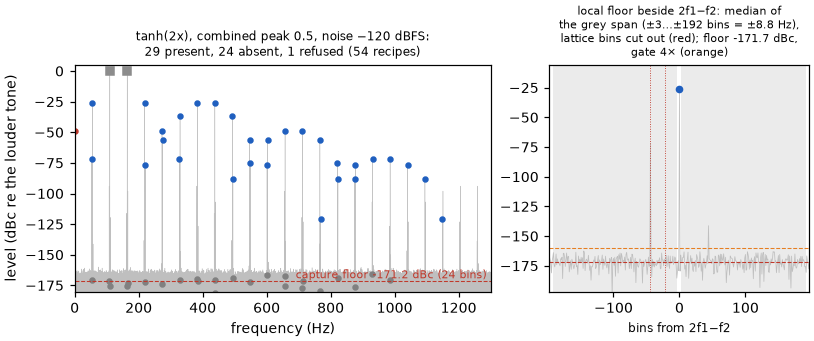
\includegraphics[width=0.95\linewidth]{imd-spectrum.png}
  \caption{The worked example, $y = \tanh(2x)$ at a combined peak of
  $0.5$ on the shipped fifth through seeded noise: the analysed spectrum
  with every enumerated product marked present (blue), absent (grey) or
  refused (red), the two tones as squares, and the capture floor as the
  dashed rule (left). Right: the local-floor neighbourhood of one product,
  the median of the grey span with every lattice bin cut out, and the gate
  four times above it.}
  \label{fig:imd-spectrum}
\end{figure}

\begin{figure}[htbp]
  \centering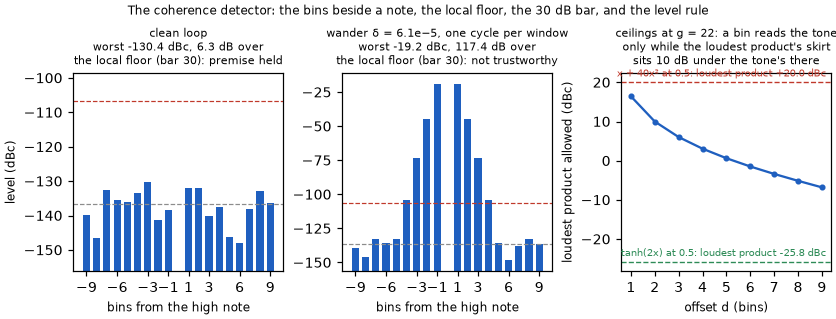
\includegraphics[width=0.95\linewidth]{imd-detector.png}
  \caption{The coherence detector beside the high note on a clean identity
  (left) and on the validated wander fixture (middle), each against the
  local floor beside the note and the bar above it; right, the per-offset
  ceilings of \eqref{eq:ceiling} on the shipped spacing, with the worked
  example's loudest product far below every ceiling and a squarer driven
  above its own tones clearing none.}
  \label{fig:imd-detector}
\end{figure}

\begin{figure}[htbp]
  \centering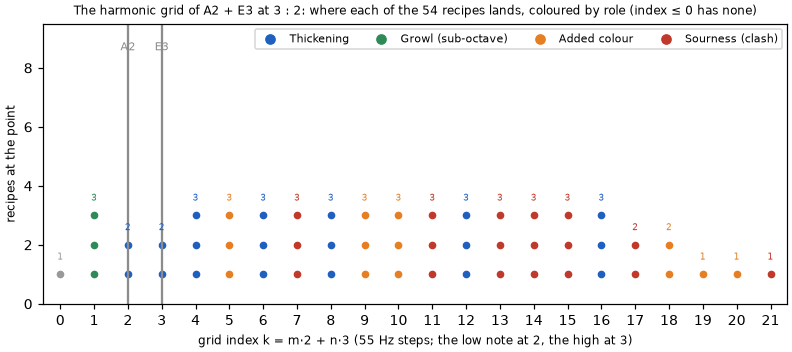
\includegraphics[width=0.95\linewidth]{imd-roles.png}
  \caption{The harmonic grid of the requested fifth at its just ratio:
  every enumerated recipe at its grid index \eqref{eq:gridindex}, stacked
  where several share a point and coloured by the role the classifier
  assigns the point; the two played notes marked. Index zero and below has
  no role.}
  \label{fig:imd-roles}
\end{figure}

The app's own rendering of the same measurement kind, from the user
guide's figure pipeline (the bundled simulated rig fed the default fifth
at the standard drive, rendered headlessly from the chart view):

\begin{figure}[htbp]
  \centering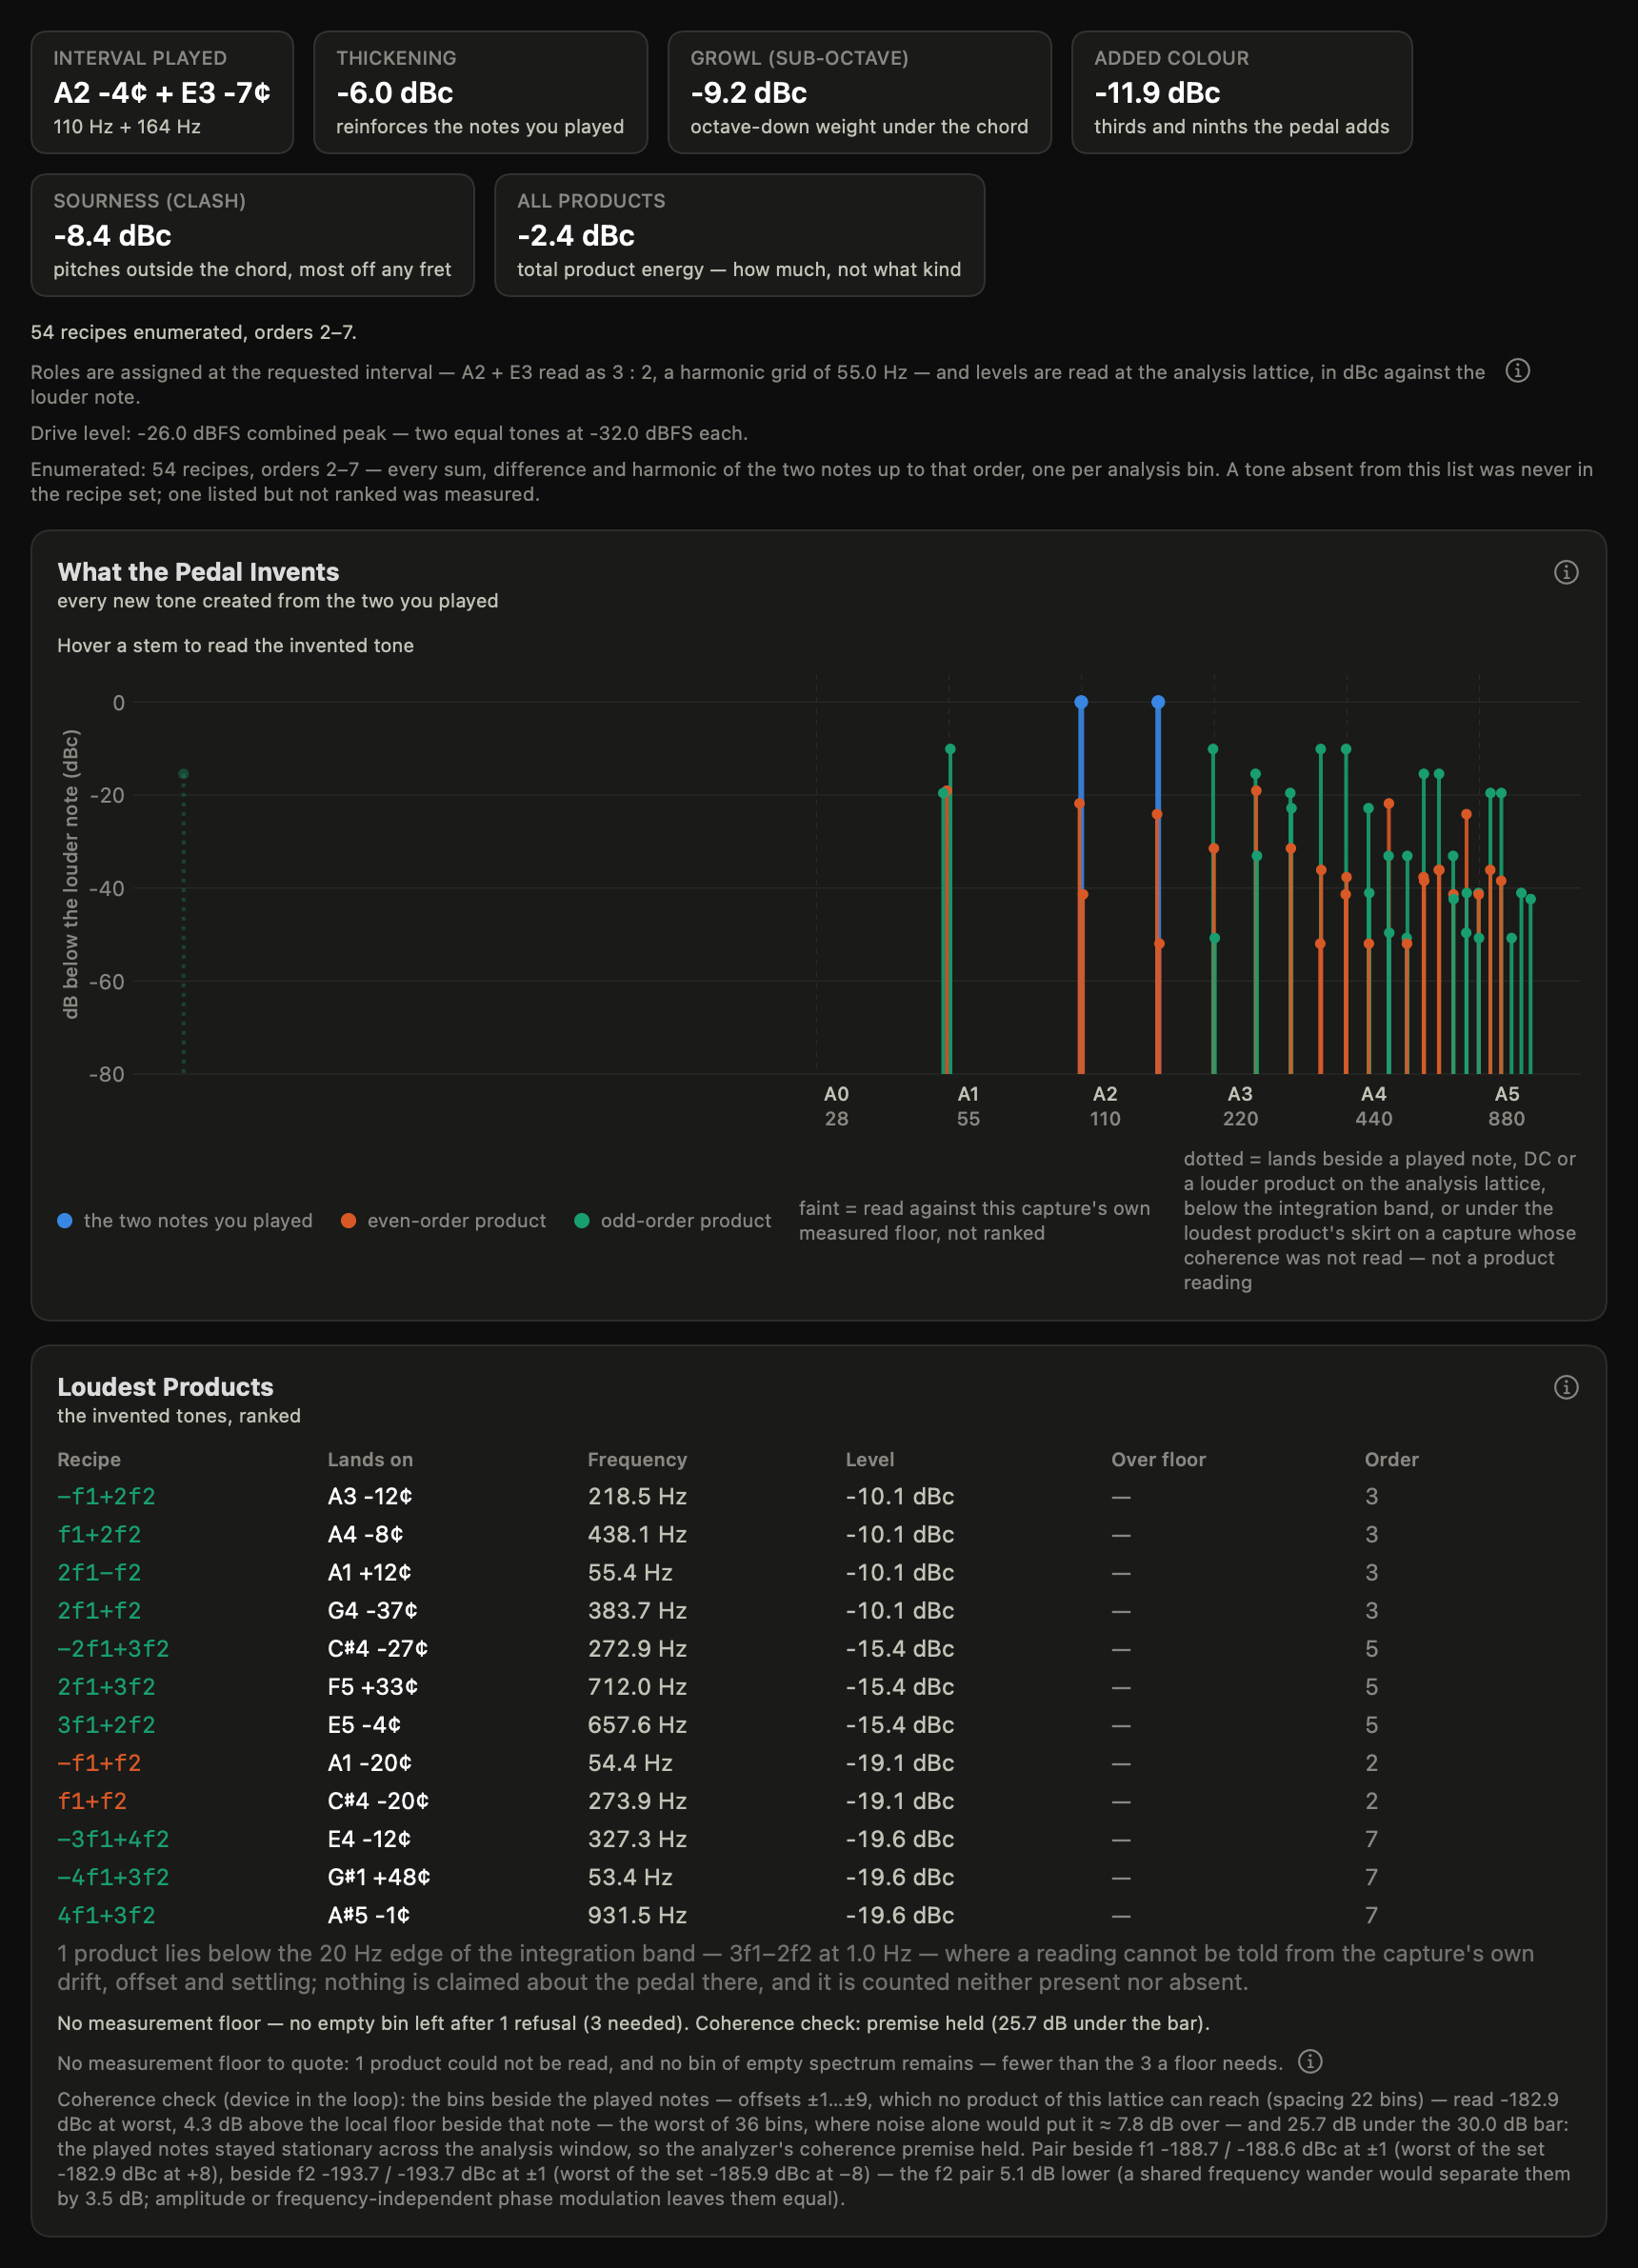
\includegraphics[width=0.85\linewidth]{chord-roughness--sim-power-chord.png}
  \caption{The Chord Roughness view as the app draws it, from the guide's
  simulated fixture: the pitch-axis spectrum, the role tiles in dBc, the
  drive line and, under the table, the floor sentence and the coherence
  line.}
\end{figure}

\subsection{Worked example and parity}
\label{sec:imd-example}
% GENERATED by gen_docs.py from a parity run (Swift vs Python vs torus-quadrature truth) — do not edit
\newcommand{\iparitySwift}{1e-07}
\newcommand{\iparitySwiftFiltered}{0.001}
\newcommand{\iparityTruthRelative}{1e-08}
\newcommand{\iparityClosedForm}{1e-09}
\newcommand{\iparityEmptyDepth}{-200}
\newcommand{\iparityTruthBandlimited}{0.001}
\newcommand{\iparityTruthKinked}{0.05}
\newcommand{\iparityTruthPhantom}{1e-08}
\newcommand{\iparityFloor}{3}
\newcommand{\iparityCoherenceNoise}{6}
\newcommand{\iparityLatencyTolerance}{1e-05}
\newcommand{\iparityCaseCount}{28}
\newcommand{\iparityTwinCount}{9}
\newcommand{\iparityWorstSwift}{1.8e-08}
\newcommand{\iparityWorstSwiftFiltered}{0.00016}
\newcommand{\iparityWorstTruthRelative}{2.6e-10}
\newcommand{\iparityWorstClosedForm}{$\le$\,1e-10}
\newcommand{\iparityWorstEmpty}{-273.8}
\newcommand{\iparityLatticeTable}{
\begin{tabular}{@{}lrrlrrrrr@{}}
\toprule case & $f_s$ & $N$ & tier & $k_1$ : $k_2$ & $g$ & $a$ : $b$ & interval (¢) & tones (¢) \\ \midrule
a-fifth-96k & 96\,000 & $2^{21}$ & standard resolvable & 2398 : 3586 & 22 & 109 : 163 & 696.65 & -3.6 / -6.94 \\
a-fifth-48k & 48\,000 & $2^{20}$ & standard resolvable & 2398 : 3586 & 22 & 109 : 163 & 696.65 & -3.6 / -6.94 \\
a-fifth-88k & 88\,200 & $2^{21}$ & standard resolvable & 2616 : 3912 & 24 & 109 : 163 & 696.65 & 0.334 / -3.01 \\
a-fifth-44k & 44\,100 & $2^{20}$ & standard resolvable & 2616 : 3912 & 24 & 109 : 163 & 696.65 & 0.334 / -3.01 \\
a-fifth-corpus & 96\,000 & $2^{17}$ & degraded & 150 : 226 & 2 & 75 : 113 & 709.63 & -2.15 / 7.48 \\
a-fifth-interactive & 48\,000 & $2^{15}$ & degraded & 75 : 113 & 1 & 75 : 113 & 709.63 & -2.15 / 7.48 \\
a-octave-96k & 96\,000 & $2^{21}$ & standard resolvable & 2418 : 4823 & 13 & 186 : 371 & 1195.3 & 10.8 / 6.12 \\
a-octave-corpus & 96\,000 & $2^{17}$ & degraded & 150 : 302 & 2 & 75 : 151 & 1211.5 & -2.15 / 9.35 \\
a-third-96k & 96\,000 & $2^{21}$ & standard resolvable & 2400 : 3024 & 48 & 50 : 63 & 400.11 & -2.15 / -2.04 \\
a-refusal & 96\,000 & $2^{16}$ & refused & 25 : 50 & 25 & 1 : 2 & 1\,200 & -4.11 / -4.11 \\
\bottomrule
\end{tabular}
}
\newcommand{\iparityDeviceTable}{
\begin{tabular}{@{}lrrrrrrl@{}}
\toprule case & content & present & S$-$P (dB) & floor (dBc) & vs truth (dB) & residue (dB) & at \\ \midrule
b-poly & 10 & 10 & 1.7e-09 & -166.84 & 7.53e-06 & $\le$\,1e-10 & 3f2 \\
b-poly-twin & 10 & 16 & $\le$\,1e-10 & -334.09 & $\le$\,1e-10 & $\le$\,1e-10 & 3f2 \\
b-squarer & 4 & 4 & 1.9e-09 & -166.53 & 2.86e-07 & $\le$\,1e-10 & 2f2 \\
b-squarer-twin & 4 & 15 & $\le$\,1e-10 & -333.84 & $\le$\,1e-10 & $\le$\,1e-10 & 2f1 \\
b-asym & 54 & 53 & 2.3e-09 & -- & 0.0298 & 0.03 & 7f1 \\
b-asym-twin & 54 & 53 & $\le$\,1e-10 & -- & 1.48e-10 & 1.5e-10 & 7f1 \\
c-tanh & 30 & 29 & 1.6e-09 & -171.17 & 0.0224 & $\le$\,1e-10 & 7f1 \\
c-tanh-twin & 30 & 33 & $\le$\,1e-10 & -318.75 & 2.91e-10 & 2.9e-10 & 7f1 \\
c-hardclip & 30 & 29 & $\le$\,1e-10 & -156.53 & 0.0128 & 0.013 & f1+4f2 \\
c-hardclip-twin & 30 & 46 & $\le$\,1e-10 & -305.72 & $\le$\,1e-10 & $\le$\,1e-10 & 5f1−2f2 \\
d-phantom & 54 & 53 & $\le$\,1e-10 & -- & 2.48e-10 & 2.5e-10 & 5f1−2f2 \\
f-squarer-hp & 4 & 4 & 0.00016 & -166.53 & 3.04e-07 & $\le$\,1e-10 & 2f2 \\
f-squarer-hp-twin & 4 & 15 & $\le$\,1e-10 & -333.82 & $\le$\,1e-10 & $\le$\,1e-10 & 2f1 \\
f-squarer-lp & 4 & 4 & 2.1e-07 & -166.53 & 2.09e-07 & $\le$\,1e-10 & 2f2 \\
f-squarer-lp-twin & 4 & 15 & $\le$\,1e-10 & -333.81 & $\le$\,1e-10 & $\le$\,1e-10 & 2f1 \\
f-tanh-prehp & 30 & 29 & 4.1e-05 & -171.17 & 0.0294 & $\le$\,1e-10 & 7f1 \\
f-tanh-prehp-twin & 30 & 33 & $\le$\,1e-10 & -318.91 & 2.96e-10 & 3e-10 & 7f1 \\
j-latency & 30 & 29 & 1.6e-09 & -171.16 & 0.0223 & $\le$\,1e-10 & 7f1 \\
j-latency-twin & 30 & 33 & $\le$\,1e-10 & -318.75 & 2.91e-10 & 2.9e-10 & 7f1 \\
\bottomrule
\end{tabular}
}
\newcommand{\iparityNoiseTable}{
\begin{tabular}{@{}lrrrrrrr@{}}
\toprule case & $N$ & noise (dBFS) & median (dBc) & floor (dBc) & bins & per-bin $-$ broadband (dB) & excess (dB) \\ \midrule
e-identity-80 & $2^{21}$ & -80 & -106.75 & -106.53 & 53 & 58.79 & 6.3 \\
e-identity-110 & $2^{21}$ & -110 & -136.75 & -136.53 & 53 & 58.79 & 6.3 \\
e-identity-corpus-80 & $2^{17}$ & -80 & -94.705 & -94.843 & 49 & 46.75 & 8.65 \\
\bottomrule
\end{tabular}
}
\newcommand{\iparityPredicateTable}{
\begin{tabular}{@{}lrrrrlrl@{}}
\toprule case & present & absent & refused & floor bins & coherence source & excess / bar (dB) & readable \\ \midrule
g-corpus-squarer & 4 & 37 & 13 & 37 & detector & 8.65 / 30 & 1..9 \\
g-corpus-cubic & 7 & 28 & 19 & 28 & detector & 8.65 / 30 & 1..9 \\
h-wander-legacy & 0 & 49 & 5 & 49 & stored products & 75.6 / 30 & 2 \\
h-wander-shipped & 0 & 53 & 1 & 53 & detector & 117 / 30 & 1..9 \\
i-loud-squarer & 4 & 0 & 50 & 49 & detector & 6.3 / 30 & none \\
\bottomrule
\end{tabular}
}
\newcommand{\iparityWorkedPresent}{29}
\newcommand{\iparityWorkedAbsent}{24}
\newcommand{\iparityWorkedFloor}{-171.2}
\newcommand{\iparityWorkedFloorBins}{24}
\newcommand{\iparityWorkedContent}{30}
\newcommand{\iparityWorkedTruthError}{0.022}
\newcommand{\iparityWorkedTruthErrorAt}{7f1}
\newcommand{\iparityWorkedResidue}{$\le$\,1e-10}
\newcommand{\iparityWorkedCoherenceExcess}{6.3}
\newcommand{\iparityWorkedLoudest}{-25.83}
\newcommand{\iparityWorkedTwoFOneMinusFTwoLevel}{-25.832}
\newcommand{\iparityWorkedTwoFOneMinusFTwoTruth}{-25.832}
\newcommand{\iparityWorkedTwoFOneMinusFTwoReading}{present}
\newcommand{\iparityWorkedTwoFTwoMinusFOneLevel}{-25.832}
\newcommand{\iparityWorkedTwoFTwoMinusFOneTruth}{-25.832}
\newcommand{\iparityWorkedTwoFTwoMinusFOneReading}{present}
\newcommand{\iparityWorkedThreeFOneLevel}{-37.078}
\newcommand{\iparityWorkedThreeFOneTruth}{-37.078}
\newcommand{\iparityWorkedThreeFOneReading}{present}
\newcommand{\iparityWorkedFOnePlusFTwoLevel}{-173.79}
\newcommand{\iparityWorkedFOnePlusFTwoTruth}{-311.15}
\newcommand{\iparityWorkedFOnePlusFTwoReading}{absent}
\newcommand{\iparityHardclipAlias}{0.0128}
\newcommand{\iparityHardclipAliasAt}{f1+4f2}
\newcommand{\iparityAsymAlias}{0.0298}
\newcommand{\iparityAsymAliasAt}{7f1}
\newcommand{\iparityAsymTwin}{1.5e-10}
\newcommand{\iparityHardclipTwin}{$\le$\,1e-10}
\newcommand{\iparityTanhTwin}{2.9e-10}
\newcommand{\iparityWorstBandlimitedResidue}{-1.2e-07}
\newcommand{\iparityPhantomWorst}{2.5e-10}
\newcommand{\iparityPhantomPresent}{53}
\newcommand{\iparityPhantomOutOfBand}{1}
\newcommand{\iparityWorstLatencyShift}{2.2e-06}
\newcommand{\iparityLatencySamples}{100}
\newcommand{\iparityPerBinLong}{58.79}
\newcommand{\iparityPerBinShort}{46.75}
\newcommand{\iparityFloorLongDeficit}{0.21}
\newcommand{\iparityFloorShortDeficit}{0.14}
\newcommand{\iparityCleanExcess}{6.3}
\newcommand{\iparityCleanExpected}{7.8}
\newcommand{\iparityWanderLegacyWorst}{-49.25}
\newcommand{\iparityWanderLegacyExcess}{75.6}
\newcommand{\iparityWanderLegacyPairDifference}{3.56}
\newcommand{\iparityWanderExpectedDifference}{3.56}
\newcommand{\iparityWanderShippedWorst}{-19.23}
\newcommand{\iparityWanderShippedExcess}{117}
\newcommand{\iparityWanderShippedPairDifference}{3.47}
\newcommand{\iparityLoudLoudest}{20}
\newcommand{\iparityLoudUnderSkirt}{49}
\newcommand{\iparityLoudSkirt}{36.8}
\newcommand{\iparityCorpusNearNote}{5}
\newcommand{\iparityCorpusNeighbour}{8}
\newcommand{\iparityCorpusFloorBins}{37}
\newcommand{\iparityPartBStatus}{Part B's parity is established: on every predicate case — the corpus lattice's refusals by position and beside a louder product, the wander fixture through the legacy path and through the detector, and the device whose products stand above its tones — the two implementations agree on every reading, every count and both registers' sentences.}


The \term{parity} runs \iparityCaseCount\ cases through both
implementations, and each device case again as its \term{phantom} twin
(\iparityTwinCount\ twins): the lattice choice alone at every standard
grid and both fallback grids, for the fifth, an octave, a major third and
a refused pair; the polynomial devices and the two clippers at the loudest
hardware drive on the shipped fifth; a phantom holding all
$\sum_{k=2}^{K} 2k$ recipes at a level ladder; the identity through seeded
noise at two levels and two lengths; a squarer behind a post-filter and
the soft clipper behind a pre-filter; the corpus lattice with a squarer
and a cubic; the wander fixture through the legacy path and through the
detector; a squarer driven until its products stand above the played
tones; and the worked example analyzed \iparityLatencySamples\ samples
late. The stimulus is the plan's own, snapped by the shipped search, so
the lattice choice is exercised, not assumed; the analysis is the app's
own call. Beside every product the oracle prints a truth: for a
memoryless device on an exact bin lattice the output is periodic on the
$(\theta_1, \theta_2)$ torus, so every product's amplitude is an exact
two-dimensional Fourier coefficient,
\begin{equation}
  a_{m,n} = 2\,|c_{m,n}|\,|H_{\mathrm{post}}(m f_1 + n f_2)|,\qquad
  c_{m,n} = \frac{1}{4\pi^2}\iint f\!\big(A_1\sin\theta_1 + A_2\sin\theta_2\big)\,e^{-i(m\theta_1 + n\theta_2)}\,d\theta_1\,d\theta_2,
  \label{eq:torus}
\end{equation}
with $A_i = a_i\,|H_{\mathrm{pre}}(f_i)|$ the drive after any pre-filter,
computed by the trapezoid rule on the grid the parameter table sizes
(exact for the periodic integrand's orders below the grid minus $K$),
never by hand; the polynomial device's closed form (the binomial expansion
in two sines) is printed beside the quadrature as a check on it; the tone
bins carry the linear response plus the odd self-terms (a cubic's
$\tfrac34 a_3 A_1^3 + \tfrac32 a_3 A_1 A_2^2$ on tone 1); the identity's
every product is zero and the phantom's are its listed levels.
\machineFloorNote{} The test asserts:
{\sloppy
\begin{itemize}
  \item Swift against Python: every header and row quantity in decibels
  within \iparitySwift\ (measured maximum \iparityWorstSwift\ on this run)
  on a capture with no filter in it, and within \iparitySwiftFiltered\
  (measured \iparityWorstSwiftFiltered) on one rendered through a biquad,
  whose direct-form recursion accumulates rounding differently in the two
  languages over two million samples; every discrete reading --- bin,
  gate, reading and its evidence, grid index, role, contest, partner ---
  identical, and every sentence identical after last-bit rounding; the two
  truths within \iparityTruthRelative\ relative (measured
  \iparityWorstTruthRelative), the closed form against the quadrature
  within \iparityClosedForm\ (measured \iparityWorstClosedForm);
  \item every analytically empty recipe on a noiseless capture at or below
  \iparityEmptyDepth\ dBc on both sides (measured worst
  \iparityWorstEmpty): the depth at which a bin-centred rectangular window
  separates nothing from the loudest component is double precision's, not
  a window's;
  \item the shipped read against the truth on every content recipe, after
  the noise allowance (a bin holds its noise too, so a read may sit up to
  $20\log_{10}(1 + 10^{(\mathrm{floor} + \mathrm{spread} - L)/20})$ from
  the truth by the noise alone): within \iparityTruthBandlimited\ for the
  bandlimited devices (measured residue at worst
  \iparityWorstBandlimitedResidue), within \iparityTruthKinked\ for the
  two kinked ones, and within \iparityTruthPhantom\ for every phantom
  (measured \iparityPhantomWorst\ on the full ladder);
  \item the lattice each case played is the row the manifest recorded by
  running the shipped search on that grid, field for field, and the
  refused pair is refused with its numbers on both sides;
  \item the identity through noise reads every product absent, its
  capture floor within \iparityFloor\ dB of the noise's analytic per-bin
  median (measured deficits \iparityFloorLongDeficit\ and
  \iparityFloorShortDeficit\ dB at the two lengths --- a median of a few
  dozen Rayleigh draws), and its coherence excess within
  \iparityCoherenceNoise\ dB of \eqref{eq:noiseexcess} (measured
  \iparityCleanExcess\ against \iparityCleanExpected);
  \item the late analysis moves the window by exactly its offset, keeps
  the overrun, and moves no content product's level by more than
  \iparityLatencyTolerance\ dB (measured \iparityWorstLatencyShift: the
  noise stream is not shifted with the window, so the late segment
  exchanges a hundred noise samples for a hundred new ones).
\end{itemize}
\par}
\iparityPartBStatus

The lattice cases --- the shipped fifth at the four rates, the two
fallback grids, the octave at two lengths, the major third, and the
refusal:

\begin{center}\scriptsize\setlength{\tabcolsep}{4pt}\iparityLatticeTable\end{center}

The device cases, each beside its alias-free twin. A twin is noiseless,
so its empty bins are numerical dust and its ``present'' count is dust
against dust --- the verdict of a noiseless case is not compared, and
the column shows why; a device case carries seeded noise far below its
content. The residue is what remains of the read's error against the truth
once the noise allowance is subtracted, clamped at zero:

\begin{center}\scriptsize\setlength{\tabcolsep}{3pt}\iparityDeviceTable\end{center}

Three readings from that table are worth stating in words. The two
\emph{kinked} devices --- the hard clip, a near-square wave whose
coefficients fall as $1/k$, and the asymmetric clipper, whose slope breaks
at zero --- applied per sample at $f_s$ fold what they make above Nyquist
back onto the lattice, where a folded high-order product lands
\emph{exactly} on a low-order bin (every lattice point is a multiple of
$g$): \iparityHardclipAlias\ dB at \iparityHardclipAliasAt\ and
\iparityAsymAlias\ dB at \iparityAsymAliasAt, against \iparityHardclipTwin\
and \iparityAsymTwin\ on their phantom twins. That is chapter one's
finding on a two-tone lattice, and the same corollary holds: a per-sample
synthetic device is never the analytic oracle for a product near the top
of the band; the phantom is. The bandlimited devices read the truth inside
the allowance on every case. And the phantom of every recipe reads back
\iparityPhantomPresent\ present and \iparityPhantomOutOfBand\ out of band
--- the recipe the shipped fifth puts under the band's low edge, whose
level still reads back to \iparityPhantomWorst\ dB and whose reading is a
refusal on frequency, by the band rule that outranks the gate.

The worked example, $y = \tanh(2x)$ at a combined peak of $0.5$ through
seeded noise: \iparityWorkedPresent\ present, \iparityWorkedAbsent\ absent,
a floor of \iparityWorkedFloor\ dBc from \iparityWorkedFloorBins\ bins, a
coherence excess of \iparityWorkedCoherenceExcess\ dB over the local
floor, and a loudest product of \iparityWorkedLoudest\ dBc. Its third-order
difference products $2f_1 - f_2$ and $2f_2 - f_1$ read
\iparityWorkedTwoFOneMinusFTwoLevel\ and \iparityWorkedTwoFTwoMinusFOneLevel\
dBc against truths of \iparityWorkedTwoFOneMinusFTwoTruth\ and
\iparityWorkedTwoFTwoMinusFOneTruth\ (both
\iparityWorkedTwoFOneMinusFTwoReading); $3f_1$ reads
\iparityWorkedThreeFOneLevel\ against \iparityWorkedThreeFOneTruth; and
the second-order $f_1 + f_2$, analytically empty for an odd device, reads
\iparityWorkedFOnePlusFTwoLevel\ dBc --- the noise --- and is
\iparityWorkedFOnePlusFTwoReading, with the bin's own level as its bound.

The identity through noise: the capture floor against the analytic median
$2\sigma\sqrt{\ln 2/N}$ of the same noise through the analyzer's scale,
and the distance of that per-bin median below the noise's broadband rms,
$10\log_{10}(N/(4\ln 2))$ --- \iparityPerBinLong\ dB at the standard
length and \iparityPerBinShort\ at the corpus length, the relation that
decides whether a broadband floor can bound a bin (it cannot without an
assumption about how the noise is spread, and the assumption is worth
tens of decibels in the refusing direction):

\begin{center}\scriptsize\setlength{\tabcolsep}{3pt}\iparityNoiseTable\end{center}

The predicate cases. On the corpus lattice a squarer through noise has
\iparityCorpusNearNote\ recipes refused beside the notes and DC and
\iparityCorpusNeighbour\ refused beside a louder product, and its floor
rests on \iparityCorpusFloorBins\ bins with those left out. The wander
fixture --- a shared fractional frequency wander of both tones, the
validated generator of the kernel's own test, which reproduces the one
real fault the reference bench has captured --- reads through the legacy
path at \iparityWanderLegacyWorst\ dBc, \iparityWanderLegacyExcess\ dB
over the capture floor, with the pair difference
\iparityWanderLegacyPairDifference\ dB against the
\iparityWanderExpectedDifference\ a frequency wander predicts; through the
detector on the shipped lattice at one cycle per window it reads
\iparityWanderShippedWorst\ dBc, \iparityWanderShippedExcess\ dB over the
local floor, over the bar in both registers. The squarer driven above its
tones has a loudest product of \iparityLoudLoudest\ dBc, clears no
ceiling, does not interpret, and marks \iparityLoudUnderSkirt\ products
unread under a skirt of \iparityLoudSkirt\ dB at the shipped spacing:

\begin{center}\scriptsize\setlength{\tabcolsep}{4pt}\iparityPredicateTable\end{center}

\subsection{Limits and failure modes}
\label{sec:imd-limits}
{\sloppy
\begin{itemize}
  \item \textbf{The floor cannot separate the device from the rig.} A
  resolved product stands above this capture's noise; the measurement
  does not say what made it. An interface's converters intermodulate, and
  a bare loop resolves a handful of second-order products of its own. The
  capture floor is the right decision floor for presence (a per-bin read
  at the product's own frequency), and the wrong instrument for
  attribution; a control capture with nothing in the loop is the only
  thing that does that job, and no rig-side broadband floor composes into
  a per-bin decision --- the per-bin median of white noise sits
  \iparityPerBinLong\ dB below the same noise's broadband rms at the
  standard length, so a broadband bound applied per bin would refuse
  genuine products by tens of decibels.
  \item \textbf{The percentage sums carry no floor bound.} The three
  capture-time sums are broadband aggregates over the products the gate
  passed, and a broadband quantity is exactly what an operative rig floor
  legitimately bounds --- so a bound is available and unbuilt: a
  percentage summed from products that each passed their own per-bin gate
  can still be quoted below what the rig supports as a whole. The
  read-time derivation subtracts refused products and bounds nothing.
  \item \textbf{A coherence verdict names no culprit, and reads nothing
  beside a loud product.} A detector bin responds to modulation of the
  played tone at periods comparable to the window itself; a pedal's
  thermal drift, a sagging supply or a dying battery moves a note as
  surely as a clock, so ``not trustworthy'' is a statement about the
  capture, never about a stage. And the check is a level rule as much as
  a distance rule: a device whose loudest product stands above the ceiling
  of \eqref{eq:ceiling} for even the nearest offset --- a full-wave
  rectifier's products stand above its own fundamentals --- is not read
  at all, and the line says why. A device whose sidebands are roughly
  constant in absolute level and fall in dBc as its output rises is
  consistent with something after the level control modulating the notes;
  the check reports the excess, the pair shape and the level, and the
  design question of whether it should say more when that dependence is
  clean is open.
  \item \textbf{What a wander looks like, and what it does not
  distinguish.} The pair statistic separates a shared fractional frequency
  wander (the pairs differ by $20\log_{10}(f_2/f_1)$, measured on the
  fixture to \iparityWanderLegacyPairDifference\ against
  \iparityWanderExpectedDifference) from amplitude or frequency-independent
  phase modulation (the pairs equal); it does not separate the latter two
  from each other, and no verdict is drawn from the shape. A $1/d$ fall
  of the sidebands with offset is the rectangular skirt of a slow,
  non-periodic drift; a lift that does not fall with offset is broadband.
  A drop in a device's even-order products between a short stimulus and
  the current long one, alongside a skirt that follows the device
  position, is consistent with an operating point that shifts over the
  window (a rectified mean through a coupling capacitor, say); the oracle
  reproduces the skirt from a stated wander and does not reproduce the
  product drop from any mechanism it models, so that half stays a bench
  question.
  \item \textbf{Aliasing in a simulated device.} A device applied per
  sample folds its content above Nyquist onto the lattice, exactly on
  low-order bins; the kinked devices' residues above quantify it. Hardware
  behind a converter's anti-alias filter does not do this.
  \item \textbf{The enumeration is a small-signal census.} Orders two
  through $K$; at the standard drive the reference clippers' content sits
  in orders two and three with trace in four and five, but a hard clipper
  at playing levels has real energy at orders the walk does not reach. An
  empty row above order five means measured and nothing above the floor at
  this drive, never that the device makes nothing there.
  \item \textbf{The corpus lattice is crowded, and every record captured
  on it carries the marks.} At the old length the fifth's spacing was two
  bins: four even-order recipes sit two bins from the played notes and one
  two bins from DC, all refused on position, and products cluster two bins
  apart so the quieter of a pair is refused beside the louder. The old
  three-bin read applies to those records too; the separation bound was
  measured under it and is deliberately not raised. On an exact small
  ratio (the original plain snap of the fifth, an exact $2 : 3$) recipes
  share bins and the surviving labels are the enumeration's tie-break,
  marked at read time as contested; those records can never be
  re-measured onto a clean lattice.
  \item \textbf{The sub-band recipe.} On the shipped fifth one recipe,
  $3f_1 - 2f_2$, lands about one hertz up: under the band's low edge,
  where nothing a pedal does can be told from the capture's own drift,
  offset and settling. It reads out of band on every record --- named in
  its own line, never in a sum, and never in a tile --- and the phantom
  parity shows the level under it still reads back exactly.
  \item \textbf{The stored gate is frozen.} The presence flag and the
  three sums are written at capture; a change to the gate's factor or the
  neighbourhood moves future captures only, and a read-time predicate can
  change which flagged bins are averaged into a floor but never which
  bins are flagged. The window length is likewise not stored: a consumer
  derives it from the stored stimulus by the plan's own rule, and a
  record captured at the old fixed length at a rate where it overran is
  asked the post-fix question and answers with no bound --- never a
  certificate that its window was clean.
  \item \textbf{The interval is a few cents off, on purpose.} Keeping the
  products separable costs pitch inside the stated budget, disclosed on
  every record; a consonant interval is a simple ratio, and a simple ratio
  is a crowded lattice, so a request that cannot escape an exact small
  ratio inside the budget is refused before anything plays rather than
  measured on a lattice whose labels are not facts.
\end{itemize}
\par}

\clearpage
\section{Glossary}
\label{sec:glossary}
Generated from \code{Docs/Methods/terms.yaml}; the plain-language companion
prints the same entries in plain language.
% GENERATED by gen_docs.py from terms.yaml — do not edit
\begin{description}
\item[{\hypertarget{term:alias-image}{alias image}}] Content above half the sample rate folds back below it in a sampled capture; order $k+1$'s image collides with the read of order $k$ once $f_0 > f_s/(2k+1)$.
\item[{\hypertarget{term:analysis-lattice}{analysis lattice}}] The set of bins the two tones and every product occupy: with tone bins $k_1 = g a$ and $k_2 = g b$ ($a : b$ coprime), the product $(m, n)$ lands on bin $m k_1 + n k_2$ exactly, so every lattice point is a multiple of $g$ and the closest two products can come is $g$ bins. Chosen once by the ratio search and scaled to each grid.
\item[{\hypertarget{term:analysis-window}{analysis window} ($N$)}] Exactly $N$ captured samples, rectangularly windowed, starting after the fade-in and the settle and ending before the fade-out; $N$ is the longest power of two under the ceiling whose segment fits the steady state, and the stimulus is sized to hold it --- 2$^{21}$ samples (21.8 s) at 96 kHz.
\item[{\hypertarget{term:analyzer-residue}{analyzer residue}}] The THD the shipped analyzer reads with nothing in the loop --- the plan's own sweep handed back as its capture --- per column of the record's grid, the worst over the sweep lengths the sheet offers, computed at read time from the record's geometry. One column above the sweep's start the fade-in ramp leaks coherently into the second-harmonic window, and a noise floor cannot see a leak that scales with the signal.
\item[{\hypertarget{term:audition-model}{audition model}}] The per-level Hammerstein fit the record carries beside the grid, consumed by the Hear-it panels only: no measured quantity reads it, and a render between two of its levels invents a bracket-shaped clipping the device does not have.
\item[{\hypertarget{term:averaged-cycle}{averaged cycle}}] The stimulus and the capture folded onto one period of the drive note in $n$ equal phase bins, each bin holding the mean of every sample whose phase fell in it, from the skipped opening cycles to the end of the tone; the figure's two coordinates are the two bins' means.
\item[{\hypertarget{term:box-normalization}{box normalization}}] Every loop area is divided by $4\,x_{\max}\,y_{\max}$, the rectangle that bounds the figure, so the areas are dimensionless and a pure ellipse from a phase shift $\varphi$ reads $(\pi/4)\,|\sin\varphi|$.
\item[{\hypertarget{term:floor-stamp}{calibration stamp}}] The embedded calibration's THD-versus-frequency curve: one read of the loopback's own distortion-plus-noise at each of a log-spaced set of fundamentals, measured once at the calibration's own drive, stored in every record.
\item[{\hypertarget{term:capture-floor}{capture floor}}] The read-time summary of a capture's empty bins: the upper median of the levels of every product judged not present and not refused on lattice position or band, with the spread above it. It bounds what the capture could see and can change no product's verdict --- one direction, no feedback.
\item[{\hypertarget{term:map-cell}{cell}}] One (level, column) of the summary grid: a THD figure over the declared band and one figure per stored harmonic order, each read from that level's own analysis at the column's fundamental.
\item[{\hypertarget{term:cleanup-reading}{cleanup reading}}] A column's THD-versus-level curve read as one of three states: the interpolated level at which it first reaches the threshold (cleans up); at or above the threshold already at the quietest level (never clean, within this map's range); under it at every level (always clean). The tile reads the column nearest the Compression probe's note.
\item[{\hypertarget{term:clipping}{clipping}}] A memoryless nonlinearity that limits the output amplitude: the output follows the input up to a threshold and is compressed or held beyond it (hard: a corner into a flat ceiling; soft: a gradual bend). An odd-symmetric clipper produces odd harmonics only; any asymmetry between the two half-cycles adds even harmonics.
\item[{\hypertarget{term:coherence}{coherence} ($\Gamma$)}] $|\sum_i z_i| / \sum_i |z_i|$ over lagged products $z_i = H(b_i + \mathrm{lag})\,\overline{H(b_i)}$: shaped content is a phasor whose phase advances smoothly with frequency, noise scatters isotropically, and the statistic is $1/\sqrt n$ for pure noise.
\item[{\hypertarget{term:coherence-check}{coherence check}}] Whether the played tones stayed stationary across the window: the worst of the detector bins beside each tone, read against the local floor beside that tone, against a measured 30 dB bar --- interpreted only over the offsets where the tone's own skirt outweighs the loudest product's, and only as a verdict about the chain, never a culprit.
\item[{\hypertarget{term:coherence-detector}{coherence detector}}] The raw spectrum at offsets $\pm 1 \ldots \pm 9$ bins beside each played tone, stored at capture with the local floor beside the tone; the widest offset is derived from the narrowest resolvable spacing ($13 - 1 - 3$), and every offset is read because an even-cycle wander lights the even ones only.
\item[{\hypertarget{term:coherent-sampling}{coherent sampling}}] Both tones complete a whole number of cycles in the analysis window, so a rectangular window leaks nothing: every product sits on one bin and the floor beneath a record is noise, not a window's skirt. The premise has no margin --- a tone that drifts during the capture spills a $1/(\pi m)$ skirt across the lattice.
\item[{\hypertarget{term:composed-margin}{composed margin}}] A cell's THD in dB over the applicable floor, the floor being the larger of the rig-noise bound (the median-read stamp with its drive term, or the operative floor) and the analyzer residue --- the larger floor is the smaller margin. Nil where neither rig source is usable.
\item[{\hypertarget{term:corroborated-peak}{corroborated peak}}] A cell that stands clear of its floor by the minimum margin AND whose neighbour one column either side --- the same level, a third of an octave away --- also stands clear; a real peak has a shoulder in frequency, a floor-riding read has none. Corroboration is never asked for in level.
\item[{\hypertarget{term:coupling-capacitor}{coupling capacitor}}] A series capacitor at a device's output: a first-order high-pass whose corner sits far below the probe note, so it removes the output's mean and leaves every harmonic's magnitude essentially untouched --- an asymmetric clipper's unequal clip levels are centred by it while its even harmonics survive.
\item[{\hypertarget{term:dbc}{dBc}}] Decibels relative to a carrier --- here the fundamental, or the louder of two played tones --- so that a product's level is stated as a ratio to the signal that produced it.
\item[{\hypertarget{term:dbfs}{dBFS}}] Decibels relative to digital full scale: $20\log_{10}$ of a linear amplitude in which $1.0$ is the largest value the converter or file can represent.
\item[{\hypertarget{term:decibel}{decibel} (dB)}] A logarithmic ratio: $20\log_{10}$ of an amplitude ratio (equivalently $10\log_{10}$ of a power ratio). $+6\dB$ doubles an amplitude, $-20\dB$ is one tenth, $-40\dB$ one hundredth; the reference is named by a suffix or by context.
\item[{\hypertarget{term:deconvolution}{deconvolution}}] Dividing the captured response's spectrum by the sweep's spectrum --- here, multiplying by the analytic inverse filter --- to recover the device's impulse response, in which the harmonic pulses appear at their time advances.
\item[{\hypertarget{term:delivered-fundamental}{delivered fundamental}}] A cell's drive level plus its stored $H_1$, in absolute dBFS. The journey's harmonic cells are uncompensated --- the loop's gain is in them --- so this is the level the fundamental actually reached at the converter, the quantity the floor's drive term compares against.
\item[{\hypertarget{term:derotation}{derotation}}] Multiplying every harmonic response by $e^{+j 2\pi f \delta / f_s}$ on its own output-frequency axis to remove a capture delay $\delta$ --- a unity-magnitude rotation, so magnitudes are untouched at every bin.
\item[{\hypertarget{term:drive-level}{drive level}}] The digital level of one level's sweep, $20\log_{10} A$ in dBFS, where $A$ is the sweep amplitude the device is driven with. On a hardware record it is the interface's output level; on a plugin record it is digital full scale itself. The lattice is a list of these.
\item[{\hypertarget{term:drive-term}{drive term}}] The floor's adjustment for a cell delivered quieter than the calibration: the stamp's ratio rises by the difference, because the rig's noise is absolute; for a cell delivered louder it stays at the stamp's own ratio --- never extrapolated past what the calibration measured, since the rig's own distortion rises with drive.
\item[{\hypertarget{term:drive-window}{drive window}}] The floor and ceiling of the lattice. The hardware window's ceiling is the loudest drive that cannot clip the converter once the input is staged for the pedal, its floor a fixed travel below; the plugin window's ceiling is digital full scale (the float render path has no converter) and its floor is lower, where high-gain preamp knees sit.
\item[{\hypertarget{term:edge-mask}{edge mask}}] The two columns that sit within a quarter tone of the grid's edges --- the sweep's fade-in and fade-out ramps --- masked from the tiles and the presence verdict; derived from the grid alone, because the artifact reproduces on a jumpered wire.
\item[{\hypertarget{term:excited-band}{excited band}}] The range of fundamentals the sweep drove at full amplitude: from the instantaneous frequency where the fade-in ends to the one where the fade-out begins. Outside it the device was driven under a ramp and a read describes the measurement, not the device.
\item[{\hypertarget{term:export-grid}{export grid}}] The summary's frequency columns: a fixed count of fundamentals log-spaced from the sweep's start to its end inclusive, so the first and last columns sit at the sweep's edges, inside its fade ramps.
\item[{\hypertarget{term:extraction-window}{extraction window} ($T_k$)}] The raised-cosine window that cuts order $k$'s pulse out of the impulse response; its half-widths are half the gap to each neighbouring pulse, capped, and its duration sets the order's spectral resolution.
\item[{\hypertarget{term:frame-fit}{frame fit}}] The single time shift $\Delta l$ between the transfer capture's alignment and the paired record's, found by maximizing the magnitude-weighted phase coherence of every fittable harmonic; its residual over the harmonics is the pairing statistic.
\item[{\hypertarget{term:fundamental}{fundamental} ($f_0$)}] The excitation frequency whose harmonics are being read; in a swept measurement every $f_0$ in the band is excited in turn, and the $k$-th harmonic of $f_0$ is read at the output frequency $k f_0$.
\item[{\hypertarget{term:fundamental-ellipse}{fundamental ellipse}}] The least-squares ellipse through the trajectory: the projection of both cycles onto the fundamental. Its area is the linear-phase loop --- what a filter's rotation of the fundamental contributes, never memory.
\item[{\hypertarget{term:fundamental-presence}{fundamental presence}}] Whether $H_1(f_0)$ is a measurement at all: absent when it sits at or beyond the analyzer's measured separation bound below the loudest valid in-band order, or at or below its rig-floor margin. Where absent, no ratio to it is quoted.
\item[{\hypertarget{term:gain-map}{gain map}}] The level-resolved harmonic measurement (§6.2's gain journey): the Harmonic Distortion sweep repeated at each drive level of a lattice, each level analyzed on its own, and the results summarized on one export grid as $\mathrm{thd}[i][j]$ and $H_k[i][j]$ --- a map of the device's distortion against level and note.
\item[{\hypertarget{term:harmonic-order}{harmonic order} ($k$)}] The integer multiple of the fundamental at which a harmonic sits; order 1 is the fundamental itself. Odd orders are produced by symmetric nonlinearities, even orders require asymmetry.
\item[{\hypertarget{term:harmonic-pulse}{harmonic pulse}}] In the deconvolved response, the impulse response belonging to one harmonic order, arriving $L \ln k$ seconds before the linear one; each is cut out with its own window.
\item[{\hypertarget{term:harmonic-response}{harmonic response} ($H_k(f)$)}] The complex, input-normalized amplitude with which the device emits energy at output frequency $f$ as its $k$-th harmonic; the harmonic of a fundamental $f_0$ is read at $f = k f_0$.
\item[{\hypertarget{term:harmonic-role}{harmonic role}}] The tiles' partition of the resolved products by what each does to the requested chord: the recipe $(m, n)$ is placed at index $m a + n b$ on the harmonic grid of the interval's simplest 5-limit just ratio $a : b$, its pitch class read off the odd part of the index; on a played note's class it thickens (at or above the low note) or adds a sub-octave; on a consonant other class it adds colour; elsewhere, or between frets, it clashes. Classified at the requested interval, measured at the lattice.
\item[{\hypertarget{term:shaping}{harmonic shaping}}] The read-time predicate deciding whether a harmonic read is content the circuit deterministically shaped or noise that landed in that order's window, from the coherence of the complex response along frequency.
\item[{\hypertarget{term:impulse-response}{impulse response} ($h[n]$)}] The deconvolved response, circular over the analysis length $N$: the linear pulse at index 0 and order $k$'s pulse at $N - \mathrm{round}(L \ln k \cdot f_s)$.
\item[{\hypertarget{term:input-normalized}{input-normalized}}] Divided by the sweep amplitude $A$, so that a unit-gain linear device reads $H_1 = 1$ (0 dB) and every $H_k$ is a ratio to the input, not an absolute level.
\item[{\hypertarget{term:instantaneous-frequency}{instantaneous frequency} ($f(t)$)}] The frequency the sweep is passing through at time $t$: $f(t) = f_1 e^{t/L}$, the derivative of the phase divided by $2\pi$.
\item[{\hypertarget{term:intermodulation-product}{intermodulation product} ($m f_1 + n f_2$)}] A component the nonlinearity places at $m f_1 + n f_2$ for integers $m, n$; its recipe is the pair $(m, n)$ and its order $|m| + |n|$ is the lowest polynomial power that can produce it. Read at one bin, exactly, and quoted in dBc re the louder played tone.
\item[{\hypertarget{term:inverse-filter}{inverse filter} ($\tilde X^{-1}(f)$)}] The closed-form stationary-phase inverse of the synchronized sweep, $2\sqrt{f/L}\,\exp(j(\pi/4 - 2\pi f L (1 - \ln(f/f_1))))$, tapered to zero below $f_1$; using the closed form extrapolates the phase law above $f_2$, so harmonics above the sweep's top deconvolve cleanly.
\item[{\hypertarget{term:just-ratio}{just ratio}}] The simplest ratio $a : b$ with every factor 2, 3 or 5 within 20 cents of the requested 12-TET interval, found by search ($3 : 2$ for the fifth, $5 : 4$ for the major third): the harmonic grid the roles are placed on has fundamental $f_1 / a$, 55 Hz for A2 + E3.
\item[{\hypertarget{term:lattice-snap}{lattice snap}}] Placing the two tones on bin centres so that a whole number of cycles of each fits the window: the reduced ratio is chosen once against every standard grid (no collisions, spacing at or above the bar, both tones inside a $\pm 15$ cent budget, then the interval nearest the request) and scaled to the grid at hand; a grid too coarse for it falls back to the widest collision-free lattice in budget, and a request that cannot escape exact degeneracy is refused before anything plays.
\item[{\hypertarget{term:lattice-spacing}{lattice spacing} ($g$)}] $\gcd(k_1, k_2)$: the integer combinations of the two tone bins are exactly the multiples of $g$ (Bézout), so no product can sit nearer than $g$ bins to another or to either tone. 22 bins on the shipped fifth at 96 and 48 kHz, 24 at 88.2 and 44.1 kHz.
\item[{\hypertarget{term:leakage-map}{leakage map}}] The parity's own instrument: the pure phantom $[1]$ --- a fundamental and nothing else --- through the journey's geometry, whose every higher-order read is the analyzer's leakage into that order's window at that column; the allowance every truth comparison subtracts.
\item[{\hypertarget{term:level-lattice}{level lattice}}] The drive levels a journey measures, evenly spaced in dB from a floor to a ceiling inclusive, one sweep per level; the hardware and plugin windows set the two ends and the level count.
\item[{\hypertarget{term:local-floor}{local floor}}] The capture-time noise estimate beside one bin: the median magnitude over the bins from 3 out to about $\pm 8.8$ Hz out on either side, with every bin the lattice claims --- products, tones, DC, the detector's bins --- removed by name. A product is called present when it stands more than four times ($12.04$ dB) above it; the verdict is stored and never revisited.
\item[{\hypertarget{term:floor}{measurement floor}}] The level below which a read is the rig rather than the device, derived at read time from the embedded calibration's pooled distortion stamp with per-track, drive and averaging adjustments; a read at or below it is reported as a bound.
\item[{\hypertarget{term:median-read}{median read}}] How the Gain Map reads the calibration stamp: each point replaced by the running median of its neighbours over an odd window before the interpolation, so a single-read trough cannot set the floor; the per-harmonic path reads the stamp verbatim (a window of one).
\item[{\hypertarget{term:memory-verdict}{memory verdict}}] The three-way reading taken on the nonlinear loop area (of the compensated figure when the phase removal is accepted): memoryless-ish below the first threshold, memory effects at and above the second, and a deliberately hedged band between them, where tone filtering ahead of the clipper rotates every harmonic by $k$ times the drive's rotation and a single fundamental cannot separate that from mild memory. Both thresholds are literals in the shipped verdict, which the manifest reads by bisection.
\item[{\hypertarget{term:lattice}{memoryless lattice}}] The set of harmonic phases $\{0, \pi\}$ (in the cycle's convention, after the Novák factor $(k-1)\pi/2$) at which a memoryless device's harmonics sit; each measured harmonic's excess over its nearest lattice point, folded consistently from low order to high, is the filter burden the removal takes out.
\item[{\hypertarget{term:manifest}{methods manifest}}] A machine-readable JSON file, emitted by the shipped measurement kernel through \texttt{analysisdump manifest}, listing every parameter that determines a measurement's result --- each value obtained by calling the function that owns it. The documents' tables are generated from it and CI fails when the committed copy drifts from a fresh one.
\item[{\hypertarget{term:nonlinear-loop-area}{nonlinear loop area}}] The unsigned lobe area of the residual trajectory after the fundamental ellipse's output is subtracted --- the harmonic content's own lobes, the headline memory figure the verdict is taken on.
\item[{\hypertarget{term:operative-floor}{operative floor}}] A plugin record's own noise bound: the larger of its silence render's rms and its A/A residual, stamped at run initiation; it enters the floor as an absolute dBFS bound with no chain-gain term, and governs where the render-path calibration is numerically silent.
\item[{\hypertarget{term:orientation}{orientation resolution}}] A plugin-path capture is aligned by correlation against a tone and may land half a cycle off; when the cycle's fundamental phase sits on the $\{0,\pi\}$ lattice and the paired polarity confidently disagrees, the output cycle is advanced half a period, restoring the true input--output pairing.
\item[{\hypertarget{term:pairing-residual}{pairing residual}}] The magnitude-weighted RMS phase residual, in radians, over the harmonics of order two and above after the frame fit; a genuine pairing sits well under the accept bar and a record of another session or setting, or a device whose harmonics have no fundamental-anchored phase relationship, does not.
\item[{\hypertarget{term:parity}{parity test}}] A continuous-integration test that runs the shipped code and the independent Python reimplementation on identical synthetic devices and asserts, at every valid point, agreement between the two to a stated tolerance and agreement of both with analytic ground truth to a stated tolerance.
\item[{\hypertarget{term:peak-tile}{peak tile}}] The map's headline figure, in three states: the loudest corroborated clear cell as a peak; else the loudest unmasked cell as a bound (``at or below''); else, when the map's fundamental is absent, no percentage at all.
\item[{\hypertarget{term:phantom}{phantom capture}}] A synthetic capture $\sum_k m_k A \sin(k\varphi(t))$ built from the sweep's own phase law, so that its $k$-th harmonic response is exactly $m_k$ by construction, with no content above the listed orders and no aliasing; the oracle's exact case.
\item[{\hypertarget{term:phase-removal}{phase removal}}] The \S\,6.5 correction: the capture's harmonic phases are fitted against the paired Harmonic Distortion record's branch phases with one frame shift, each harmonic's burden over the memoryless lattice is folded out sequentially, and the correction is applied as a full-band unity-magnitude all-pass, so filter phase before and after the clipper is removed and only unpredicted phase --- memory evidence --- remains.
\item[{\hypertarget{term:polarity}{polarity}}] Whether the device inverts: read from the paired record's $H_1$ as the energy-weighted mean unit phasor over the low band, whose real part is the confidence (a quadrature response is coherent yet polarity-mute); stated on the figure only when the frame fit confirms the pairing.
\item[{\hypertarget{term:gate}{presence gate}}] The analyzer's per-bin criterion, amplitude $> 4 \times$ the local floor ($20 \log_{10} 4 = 12.04$ dB), decided at capture and frozen in the payload as the product's \texttt{aboveFloor} flag.
\item[{\hypertarget{term:product-order}{product order} ($|m| + |n|$)}] The order of the recipe $(m, n)$: the polynomial power that first produces it. The analyzer enumerates every recipe of order two through seven --- 54 on a lattice with no collisions --- and a shared bin is kept by its lowest order.
\item[{\hypertarget{term:product-reading}{product reading}}] One of four outcomes per product, decided in a fixed order: refused on lattice position (beside a played tone or DC), out of band (under 20 Hz), refused beside a louder product, refused by the analyzer's window or under the loudest product's skirt, then present with its margin over the capture floor or absent with the bin's own read as a bound. A refusal is never silently absent.
\item[{\hypertarget{term:rate-constant}{rate constant} ($L$)}] The time in seconds over which the sweep's instantaneous frequency grows by a factor of $e$: $f(t) = f_1 e^{t/L}$. Fixed by the synchronization condition from the requested duration.
\item[{\hypertarget{term:scatter}{read scatter}}] The one-sigma uncertainty, in dB, of a magnitude read at its estimated signal-to-noise ratio --- the Rician mean-of-dB statistic, pinned by a Monte-Carlo table and saturating at the pure-noise value.
\item[{\hypertarget{term:reduced-ratio}{reduced tone ratio} ($a : b$)}] The tone bins in lowest terms. Two recipes of order at most $K$ can share a bin only when $a + b \le 2K$, so the probe insists on $a + b \ge 2K + 1$; the ratio alone fixes the delivered interval, whatever the rate or length. The shipped fifth is $109 : 163$.
\item[{\hypertarget{term:alignment-error}{residual alignment error}}] Any difference between the integer loop latency removed before binning and the true delay, in samples; it rotates the output's fundamental by $2\pi f_0 e/f_s$ and harmonic $k$ by $k$ times that, opening the figure into a phase loop that grows with the note.
\item[{\hypertarget{term:pair-statistic}{sideband pair statistic}}] The mean of the two innermost detector bins about each tone, and the difference between the two tones' pairs against $20 \log_{10}(f_2 / f_1)$: a shared fractional frequency wander separates the pairs by that figure, while amplitude or frequency-independent phase modulation leaves them equal --- a shape the line states without a verdict.
\item[{\hypertarget{term:static-curve}{static curve}}] The output-versus-input estimate that ignores the loop: the cycle is split at the input's extremes into a rising and a falling branch, each is interpolated onto a common input grid, and the two are averaged --- never binned by input value.
\item[{\hypertarget{term:averaging}{sweep averaging}}] Combining $N$ back-to-back sweeps from one capture by complex, bin-wise averaging of their harmonic responses after each repeat is derotated by its fitted capture delay; the noise power falls as $1/N$ where the residual is noise, and magnitudes are never averaged.
\item[{\hypertarget{term:synchronization}{synchronization condition}}] The requirement that $f_1 L$ be an integer, met by rounding the rate constant; it makes the sweep's phase at every harmonic's arrival a whole number of cycles, so harmonic responses separate with meaningful phase.
\item[{\hypertarget{term:sweep}{synchronized swept sine} ($x(t)$)}] A sine whose frequency rises exponentially from $f_1$ to $f_2$ over the duration $T$, with its rate constant chosen so that $f_1 L$ is an integer; under that condition each harmonic a memoryless device generates is an exact time-advanced copy of the sweep, advanced by $L\ln k$.
\item[{\hypertarget{term:tanh}{tanh}}] The hyperbolic tangent, as the saturating function $y = \tanh(g x)$: linear for small inputs and bending smoothly toward $\pm 1$, which it never reaches --- the textbook soft clipper. It is odd-symmetric, so it produces odd harmonics only, and its ladder falls off steeply with order. The worked example throughout these documents is $\tanh(2x)$ at a sweep amplitude of $0.5$, whose exact harmonic amplitudes are computed by quadrature.
\item[{\hypertarget{term:thd}{total harmonic distortion} ($\mathrm{THD}$)}] $\sqrt{\sum_{k \ge 2} |H_k(k f_0)|^2} / |H_1(f_0)|$ over the orders that are in the audible band and pass the validity bound --- THD, not THD+N; undefined where the fundamental is not present.
\item[{\hypertarget{term:transfer-curve}{transfer curve}}] The X--Y figure of a device under a steady low-frequency sine: instantaneous output against instantaneous input over one phase-averaged cycle. A memoryless device retraces a single curve; linear filter phase and genuine memory open it into a loop.
\item[{\hypertarget{term:truncated-column}{truncated column}}] A column where the validity bound removed an order that the declared band would have counted, so its THD cells under-read their band; the column is flagged and excluded from the tiles, never corrected.
\item[{\hypertarget{term:two-tone}{two-tone measurement}}] Chord IMD: two simultaneous sines at a musical interval, snapped to exact bins of the analysis window, driven through the device; the result is the level of every intermodulation product up to the seventh order, the three capture-time percentage sums, and the coherence detector's reads beside each tone.
\item[{\hypertarget{term:lobe-area}{unsigned lobe area}}] The total loop area: the closed trajectory is split at every self-crossing and the absolute area of every lobe is summed, so opposite-winding lobes add instead of cancelling; lobes under a floor fraction of the box are dropped as bin noise.
\item[{\hypertarget{term:validity-bound}{validity bound}}] Where a harmonic read is trustworthy: $f_1 \le f_0 \le f_2$ and $f_0 \le f_s/(2k+1)$ (the alias-image bound), plus $f_0 \le f_{\mathrm{cal}}/k$ on a compensated record. Reads outside it are excluded from every fit, feature, summary and comparison.
\end{description}


\clearpage
\appendix
\section{Scripts, tests and how to reproduce}
Paths are relative to \code{Docs/Methods/} in the repository, except the
tool, which lives under \code{Tools/}. The repository: \repo

\begin{longtable}{@{}p{0.34\linewidth}p{0.62\linewidth}@{}}
\toprule Path & Role \\ \midrule \endhead
\code{Tools/analysisdump} & the shipped-code oracle: \code{synth} (a known device through the shipped analyzer, with exact truth beside it), \code{transfer-synth} (a known device through the shipped transfer path, paired, with its truth beside it), \code{compression-synth} (a known device through a known loop and the shipped Compression path inside the app's assembly, the ladder beside every step), \code{journey-synth} (a known device through a known loop and the shipped Gain Map path, the ladder beside every cell), \code{imd-synth} (a known device or a phantom through the shipped two-tone path, with the torus-quadrature truth beside every product), \code{windows}, \code{manifest} \\
\code{generated/manifest.json} & the manifest, committed, drift-checked \\
\code{py/harmonic\_distortion.py} & the reimplementation; \code{--help} lists the same options as \code{synth} \\
\code{py/parity\_hd.py} & the comparison and the tolerances, with their provenance \\
\code{py/test\_parity\_hd.py} & the CI parity test (pytest) \\
\code{py/transfer\_curve.py} & the Transfer Curve reimplementation (the options of \code{transfer-synth}) \\
\code{py/parity\_transfer.py} & its comparison and tolerances, with provenance \\
\code{py/test\_parity\_transfer.py} & its CI parity test \\
\code{py/compression\_curve.py} & the Compression reimplementation (the options of \code{compression-synth}); imports \code{harmonic\_distortion.py} and \code{transfer\_curve.py} \\
\code{py/parity\_compression.py} & its comparison and tolerances, with provenance \\
\code{py/test\_parity\_compression.py} & its CI parity test \\
\code{py/gain\_map.py} & the Gain Map reimplementation (the options of \code{journey-synth}); imports \code{harmonic\_distortion.py} \\
\code{py/parity\_journey.py} & its comparison and tolerances, with provenance \\
\code{py/test\_parity\_journey.py} & its CI parity test \\
\code{py/chord\_imd.py} & the Chord IMD reimplementation (the options of \code{imd-synth}) \\
\code{py/parity\_imd.py} & its comparison and tolerances, with provenance \\
\code{py/test\_parity\_imd.py} & its CI parity test \\
\code{py/make\_figures.py} & the figures, seeded, byte-stable, with TSV sidecars of the plotted values \\
\code{py/gen\_docs.py} & the generated fragments this document inputs \\
\code{terms.yaml} & the terms source; \code{py/test\_terms.py} is its guard \\
\code{make methods-test} & parity and terms guards \\
\code{make methods-docs} & manifest $\to$ figures $\to$ fragments $\to$ both PDFs \\
\bottomrule
\end{longtable}

Toolchain: Python 3 with the versions pinned in
\code{Docs/Methods/requirements.txt}; \LaTeX\ through \code{latexmk} with
\code{pdflatex}, pinned in \code{Docs/Methods/tex/latexmkrc}. The Swift
tool builds with the repository's own toolchain.

\bibliographystyle{plainnat}
\bibliography{references}
\end{document}
